\documentclass[preprint,12pt]{elsarticle}

%% Use the option review to obtain double line spacing
%% \documentclass[preprint,review,12pt]{elsarticle}

%% Use the options 1p,twocolumn; 3p; 3p,twocolumn; 5p; or 5p,twocolumn
%% for a journal layout:
%% \documentclass[final,1p,times]{elsarticle}
%% \documentclass[final,1p,times,twocolumn]{elsarticle}
%% \documentclass[final,3p,times]{elsarticle}
%% \documentclass[final,3p,times,twocolumn]{elsarticle}
%% \documentclass[final,5p,times]{elsarticle}
%% \documentclass[final,5p,times,twocolumn]{elsarticle}

%% The graphicx package provides the includegraphics command.
\usepackage{graphicx}
%% The amssymb package provides various useful mathematical symbols
\usepackage{amssymb}
\usepackage{amsmath}
\usepackage{breqn}
\usepackage{chemfig}
\usepackage{csvsimple}
%% The amsthm package provides extended theorem environments
%% \usepackage{amsthm}

%% The lineno packages adds line numbers. Start line numbering with
%% \begin{linenumbers}, end it with \end{linenumbers}. Or switch it on
%% for the whole article with \linenumbers after \end{frontmatter}.
\usepackage{lineno}
\usepackage{natbib}
\usepackage{hyperref}
% \usepackage[top=0.75in, bottom=0.75in, left=0.55in, right=0.85in]{geometry}
\usepackage{graphicx}
\usepackage{url}
\usepackage{palatino}
\usepackage{tabularx}
\usepackage{graphicx}
\usepackage{multicol}
\usepackage{graphicx}
\usepackage{amssymb}
\usepackage{float}
\usepackage{amsmath}
\usepackage{rotating}
\usepackage{subfigure}
\usepackage{multirow}
\usepackage{mathrsfs}
\usepackage{xfrac}
\usepackage[font=small,skip=0pt]{caption}
%\usepackage[numbers,sort&compress]{natbib}
%\usepackage{hyperref}
\usepackage{pgf,tikz}
\usetikzlibrary{shapes,arrows,chains}
\usetikzlibrary[calc]
\usepackage{graphicx}
\graphicspath{ {./images/} {./images/clusterHistogram/cluster1/}{./images/clusterHistogram/cluster0/}{./images/clusterHistogram/cluster2/}{./images/allFuelFinal/}{./images/noHexaneHexa/}{./images/3fuel/}}

\usepackage{geometry}
\geometry{lmargin=1in,rmargin=1in,tmargin=1in,bmargin=1in}
\usepackage{lipsum}
%\pagestyle{empty}
\usepackage{natbib}
\pagenumbering{arabic}
%\usepackage[T1]{fontenc}
\usepackage{setspace}
\usepackage{mathptmx}
\usepackage{t1enc}
%\usepackage{xkeyval}
%\usepackage{chemformula}
%\usepackage{array}
%\usepackage{booktabs}
%\usepackage{hypdoc}
%\usepackage{listings}
%\usepackage{lmodern}
%\usepackage{mathpazo}
%\usepackage{microtype}
\usepackage{graphicx}
\usepackage{amssymb}
\usepackage{float}
\usepackage{amsmath}
\usepackage{rotating}
\usepackage{subfigure}
\usepackage{multirow}
\usepackage{xfrac}
\usepackage[font=small,skip=0pt]{caption}
%\usepackage[numbers,sort&compress]{natbib}
%\usepackage{hyperref}
\usepackage{pgf,tikz}
\usetikzlibrary{shapes,arrows,chains}
\usetikzlibrary[calc]
\usepackage{graphicx}
\usepackage{geometry}
\geometry{lmargin=1in,rmargin=1in,tmargin=1in,bmargin=1in}
\usepackage{lipsum}
%\pagestyle{empty}
\usepackage{natbib}
\pagenumbering{arabic}
%\usepackage[T1]{fontenc}
\usepackage{setspace}
\usepackage{mathptmx}
\usepackage{t1enc}
%\usepackage{xkeyval}
%\usepackage{chemformula}
%\usepackage{array}
%\usepackage{booktabs}
%\usepackage{hypdoc}
%\usepackage{listings}
%\usepackage{lmodern}
%\usepackage{mathpazo}
%\usepackage{microtype}
\usepackage{lineno,hyperref}
\usepackage{multirow}
\usepackage{cancel}
\usepackage{url}
\usepackage[norule]{footmisc}
\usepackage[utf8]{inputenc}
\usepackage[english]{babel}
\hypersetup{colorlinks = true,linkcolor = blue,urlcolor = blue}
% \fontfamily{SansSerif}
% \selectfont
% \usepackage[T1]{fontenc}
% \usepackage
%% natbib.sty is loaded by default. However, natbib options can be
%% provided with \biboptions{...} command. Following options are
%% valid:
%%   round  -  round parentheses are used (default)
%%   square -  square brackets are used   [option]
%%   curly  -  curly braces are used      {option}
%%   angle  -  angle brackets are used    <option>
%%   semicolon  -  multiple citations separated by semi-colon
%%   colon  - same as semicolon, an earlier confusion
%%   comma  -  separated by comma
%%   numbers-  selects numerical citations
%%   super  -  numerical citations as superscripts
%%   sort   -  sorts multiple citations according to order in ref. list
%%   sort&compress   -  like sort, but also compresses numerical citations
%%   compress - compresses without sorting
%%
%% \biboptions{comma,round}
% \biboptions{}

\usepackage{caption}
\usepackage{algorithm} 
\usepackage[noend]{algpseudocode}
\usepackage{amsmath}
\DeclareMathOperator*{\argmin}{argmin}
\DeclareMathOperator*{\argmax}{argmax}
\newcommand*{\argminl}{\argmin\limits}
\newcommand*{\argmaxl}{\argmax\limits}



\journal{Journal Name}
\begin{document}
	
	\begin{frontmatter}
		
		%% Title, authors and addresses
		
		\title{Prediction of ignition delay using data-driven framework for straight chain alkanes}
		
		%% use the tnoteref command within \title for footnotes;
		%% use the tnotetext command for the associated footnote;
		%% use the fnref command within \author or \address for footnotes;
		%% use the fntext command for the associated footnote;
		%% use the corref command within \author for corresponding author footnotes;
		%% use the cortext command for the associated footnote;
		%% use the ead command for the email address,
		%% and the form \ead[url] for the home page:
		%%
		%% \title{Title\tnoteref{label1}}
		%% \tnotetext[label1]{}
		%% \author{Name\corref{cor1}\fnref{label2}}
		%% \ead{email address}
		%% \ead[url]{home page}
		%% \fntext[label2]{}
		%% \cortext[cor1]{}
		%% \address{Address\fnref{label3}}
		%% \fntext[label3]{}
		
		
		%% use optional labels to link authors explicitly to addresses:
		%% \author[label1,label2]{<author name>}
		%% \address[label1]{<address>}
		%% \address[label2]{<address>}
		
		\author{Pragneshkumar Rana, Sivaram Ambikasaran, Krithika Narayanaswamy \\ 
			(Not sure about order: last considered  as main guide and principal supervisor) }
		
		\address{Indian Institute of Technology, Madras}
		
		\begin{abstract}
			%% Text of abstract
		 Ignition delay is important global combustion property. Ignition delay time(IDT) is generally measured using Shock-tube and RCM experiments. Calculation of IDT from numerical reacting simulation is computationally costly and time consuming process. To obtain IDT faster and accurately, shock tube experimental data is used to predict IDT using machine learning algorithms. Generally, IDT correlation is Arrhenius type in its nature which reformulated using bond energy. Rather than activation energy, fuel bond information is used to avoid uncertainty and dependency of experimental parameters. To predict IDT, by k-means algorithm, dataset is divided into sub-dataset by Euclidean norm minimization. Optimum number of sub dataset(data clusters) is obtained using  silhouette criteria. For each sub-dataset, using multiple regression and hypothesis testing final correlation and framework obtained to predict IDT for unknown fuel. Result obtained  using framework and correlation shows excellent agreement with experimental result.  
		\end{abstract}
		
		\begin{keyword}
			Ignition delay prediction \sep Machine learning \sep Data-Driven , K-Means, Silhouette Criteria, IDT correlation, Framework
			%% keywords here, in the form: keyword \sep keyword
			
			%% MSC codes here, in the form: \MSC code \sep code
			%% or \MSC[2008] code \sep code (2000 is the default)
		\end{keyword}
		
	\end{frontmatter}
	
	%%
	%% Start line numbering here if you want
	%%
	\linenumbers
	
	%% main text
	\section{Introduction:}
	\label{S:1}
	Combustion process is mainly characterized by transport processes and chemical reactions. When fluid undergoes chemical reaction, it liberates heat without external source of energy such that process sustains, which is called as Ignition. Ignition comprises series of coincidental physical and chemical processes which have different characteristic time scale, which is called as ignition delay. 
	
	Ignition delay is physio-chemical property. It is one of the major global combustion property. Ignition delay gives important information about fuel reactivity and ignition. Ignition delay is mainly comprised of two parts: physical ignition delay and chemical ignition delay. Physical ignition delay depends on certain physical phenomena such as heating, fuel atomization, penetration of spray, and evaporation rate of fuel for different temperature range. Whereas, chemical ignition delay is mainly function of chemical characteristics of fuel, molecular structure, equivalence ratio, etc. The main focus of this study is chemical ignition delay. Henceforth, chemical ignition delay will be referred as Ignition delay(ID).  Apart from chemical characteristics of fuel, Ignition delay is also function of pressure, temperature as reaction rates are also function of same.

		
		Ignition delay is crucial factor for design of combustor. Right amount of ignition delay time is required for proper combustion. Prediction of IDT for various fuel and wide range of conditions is complicated process. Ignition delay are generally calculated using reacting flow simulation which involves large number species and thousands of reaction including broad range of chemical and flow time scale. Prediction of IDT using realistic fuel chemistry requires large scale simulations of combustion phenomena \cite{computation}. Ignition delay solution using realistic-detail mechanism  requires full-scale chemistry solvers which are computationally intensive. Taking motivation from such complications, acquired framework and correlations are simplified, accurate, and efficient which is  applicable over variety of fuels and wide range of conditions. 
			
		For development and validation of predictive reaction models, ignition data are very useful. Substantial work has been done by researchers to calculate and correlate the ignition delay. Major ignition delay equations are based on Arrhenius-type correlation which can be written as~\cite{goldsborough2009chemical}:
		\begin{equation}
		\tau = A \phi^\alpha P^\beta X_{O_2}^\gamma exp(\lambda)
		\end{equation}
		$\alpha, \beta, \gamma$ are polynomials, to capture changes in functionality across different regimes. $\lambda$ is overall activation energy. Horning et al.~\cite{horning} has conducted study of different hydrocarbon at high-temperature to observe auto ignition and thermal decomposition. He found that for n-alkanes at $\phi =1$ follows the given ignition delay correlation-\ref{eq:horning_eq}
		\begin{equation}\label{eq:horning_eq}
		\tau = 9.40  * \space 10^{-6} P^{-0.55} X_{Oxi}^{0.63} C^{-0.5} e^{46500/RT}
		\end{equation}
		
		Where C is number of carbon atoms in the molecules. Such Arrhenius-type equations are constrained based on certain physical condition. In parametric uncertainty~\cite{horning}, it was mentioned that activation energy is very sensitive to ignition temperature which directed to find out more efficient parameter to replace activation energy. 
		
			\vspace{1 mm}
			\textbf{Notations :}
			
			\begin{table}[htpb!]\label{table:Notation}
				\begin{tabular}{ l l }	
					P = Pressure &	T = Temperature \\
					$\phi$ = Equivalence Ratio & $\tau$ = Ignition Delay Time \\
					$X_{Oxi}$ = Oxidizer mole fraction &  $X_{Fuel}$ = Fuel mole fraction   \\
					$E_a$ = Activation Energy & $\delta H$ = Change in enthalpy \\
					R = Gas constant & 		A = Scaling factor \\
					IDT = Ignition delay time & C = Constant \\
				\end{tabular}
			\end{table}
			\vspace{3mm}
		
		In recent study of distillate fuels, Fethi and Amir \cite{khaled2019universality} has obtained ignition delay correlation for gasoline and Jet-Fuel using modified Arrhenius expression which applicable over wide range of conditions  [P = 10-80 bar, $P_0$ = 1 bar, $\phi$ = 0.5-2, fuel/air mixtures, units are ms, bar, K, mol, kcal]. Using chemical model of Sarathy at el. and by montecarlo simulation they generated $10^7$ samples. Using those samples and by statistical approach they found the correlation [\ref{eq:ID}]:	
		\begin{equation} \label{eq:ID}
		\begin{split}
		\tau_{gasoline} = 6.76*10^-7\frac{P}{20}^{-1.01} \phi^{1.13 - \frac{(17.59)}{T}} \exp{\frac{29.39}{RT}}\\			\newline
		for T > \frac{1000}{-0.073 ln(\frac{P}{P_0})+ \phi^{-0.0338} + 0.0938}\\
		\tau_{JetFuel} = 4.76*10^-7\frac{P}{20}^{-1.21} \phi^{2.04 - \frac{(29.56)}{T}} \exp{\frac{29.33}{RT}}\\			\newline
		for T > \frac{1000}{-0.0371 ln(\frac{P}{P_0})+ \phi^{-0.00727} + 0.0995}
		\end{split}
		\end{equation}
		Such correlations are useful for modelling of the surrogates. But such correlations are fuel specific and constrained by physical conditions so it is  quite difficult to obtain IDT for new fuel or surrogates.\textbf{ The goal} of present study is to find out correlation which generalize, efficient, applicable over wide range physical condition and variety of fuel. To obtain this, it is necessary to modify Arrhenius-type equation. In next section, ignition delay formulation has been discussed which is further used to find out coefficient using machine learning approach. 
		
		\subsection{Ignition delay formulation:}
		
		As we discussed earlier, many researchers have obtained IDT correlation from Arrhenius-type formulation. But specificity of fuel and physical parameter causes uncertainty in result of IDT. To remove such complication, ignition delay correlation has to be reformulated. 
		
		In chemical reactions, the most sensitive parameter in ignition delay correlation is Activation energy. Activation energy describes overall transformation of reaction and it only gives macroscopic information about reaction as intermediates are not considered in any reaction. More microscopic information about the single step reaction can be obtained using the Eyring eqaution~\cite{modernbook}.
		\begin{equation}\label{eyring}
		k = \kappa\bigg( \frac{k_BT}{h} \bigg) e^{\frac{\Delta S^{\ddagger}}{R}} e^{\frac{-\Delta H^{\ddagger}}{RT}}
		\end{equation} 
		Where, $k_B$ = Boltzmann constant, T = absolute temperature, h = Planck's constant, $\Delta S^{\ddagger}$ = Activation Entropy, $\Delta H^{\ddagger}$ = Activation Enthalpy. Eyring's equation is based on statistical and mechanical rationale of transition state theory whereas Arrhenius equation is empirical. These both equation are different in its nature. Relation between these two equations is possible when elementary reaction is as uni-molecular or bi-molecular. In such case, activation energy or  Energy barrier can be defined in terms of enthalpy of activation~\cite{modernbook} which is closely related to bond energy.
		\begin{equation}\label{acti_entha}
		E_a = \Delta H^{\ddagger} + nRT
		\end{equation}
		
		 According to transition state theory, when molecules with enough kinetic energy collides in certain orientation, it may generate activated complex. Bond structure of activated complex  is different from reactants bond structure. $\Delta H^{\ddagger}$ plays critical role in bond formation or breakage.So, enthalpy of activated complex is related to enthalpy of reaction. 
		 
		 In combustion, heat of combustion  ($\Delta H_{combustion}$) or heat of reaction  ($\Delta H_{reaction}$ = -$\Delta H_{combustion}$) is directly related to bond dissociation energy \cite{bond_energy} which can be expressed as,
		\begin{equation}\label{enth_form}
		\begin{aligned}
		\Delta H_{combustion} &= H_{reactants} - H_{products} \\
		&\approx \text{Bond energy of Reactants}- \text{Bond energy of Products}
		\end{aligned}
		\end{equation}
		Being point function, enthalpy of activation ($\Delta H^\ddagger$) for forward reaction can be expressed as difference between reactant state and activation state,
		\begin{equation}\label{enth_acti1}
		\begin{aligned}
		\Delta H^{\ddagger} &= H_{reactant} - H^{\ddagger} \\
		\end{aligned}
		\end{equation}
		from relation-(\ref{enth_form}),
		\begin{equation}\label{enth_acti2}
		\begin{aligned}
		\Delta H^{\ddagger} &=\Delta H_{combustion} + H_{products} - H^{\ddagger} \\
		\end{aligned}
		\end{equation}
		%  As mentioned earlier  $H_{products}$ and $H^{\ddagger}$ are point functions so, their value will be specific related to that state which can be replace by some constant B.
		% \begin{equation}\label{enth_acti3}
		%     \begin{aligned}
		%  \Delta H^{\ddagger} &=\Delta H_{combustion} + B \\
		% \end{aligned}
		% \end{equation}
		In IDT relation-(\ref{eq:horning_eq}) Horning et al. has showed that IDT depends on the number of carbons. So, Arrhenius-type ignition delay formulation can be written as below using equation-(\ref{acti_entha}) and (\ref{enth_acti2}). 
		\begin{equation}
		\begin{aligned}
		\tau &= A \cdot \phi^\alpha  \cdot P^\beta  \cdot X_{O_2}^\gamma  \cdot exp\bigg(\frac{E_a}{RT}\bigg) \\
		&= A \cdot \phi^\alpha \cdot P^\beta  \cdot X_{O_2}^\gamma  \cdot exp\bigg(\frac{\Delta H^{\ddagger} + nRT}{RT}\bigg) \\
		&= A \cdot \phi^\alpha  \cdot P^\beta  \cdot X_{O_2}^\gamma  \cdot exp\bigg(\frac{\Delta H_{combustion} + H_{products} - H^{\ddagger}}{RT}\bigg)exp\bigg(\frac{nRT}{RT}\bigg) \\
		&= A \cdot exp(n) \cdot \phi^\alpha  \cdot P^\beta  \cdot X_{O_2}^\gamma   \cdot exp\bigg(\frac{\Delta H_{combustion} + H_{products} - H^{\ddagger}}{RT}\bigg) \\
		&= C \cdot \phi^\alpha  \cdot P^\beta  \cdot X_{O_2}^\gamma  \cdot exp\bigg(\frac{\Delta H_{combustion} + H_{products} - H^{\ddagger}}{RT}\bigg) \\
		\end{aligned}
		\end{equation}
		From-\ref{enth_form}, it clear that enthalpy of combustion depends on the type of bond and bond energy. Other enthalpy details are constant being point function so, formulation can be rewritten as,
		\begin{equation}\label{eq:formulation}
		\begin{aligned}		
			&\propto  \phi^\alpha \cdot P^\beta  \cdot X_{O_2}^\gamma   \cdot exp\bigg(\frac{\text{ Fuel Bond Energy}\cdot \text{Constant}}{T}\bigg) \\
			&\propto  \phi^\alpha \cdot P^\beta  \cdot X_{O_2}^\gamma   \cdot exp\Bigg(\small{\frac{ \sum_{i=1}^{n} \text{(Bond Type)}_i \cdot \text{(Bond Energy)}_i \cdot \text{Constant} }{T}} \Bigg) \\
			&\propto  \phi^\alpha \cdot P^\beta  \cdot X_{O_2}^\gamma   \cdot exp\Bigg(\small{\frac{ \sum_{i=1}^{n}\text{(Bond Type)}_i \cdot \text{(Bond Energy $\cdot$ Constant)}_i}{T}} \Bigg) \\
			&\propto  \phi^\alpha \cdot P^\beta  \cdot X_{O_2}^\gamma   \cdot exp\Bigg(\small{\frac{ \sum_{i=1}^{n}\text{(Bond Type)}_i \cdot \text{(Bond Constant)}_i}{T}} \Bigg) 
			\end{aligned}
		\end{equation}
		
		Bond constant has unit of K/J which is inverse of universal gas constant. This formulation gives indication that ignition delay depends on the chemical bonds of the fuel. Further in the formulation, to make quantities independent of unit, it was normalized with standard conditions. Considering all the affecting parameters in above formulation-\ref{eq:formulation} hypothetical functional form of IDT can be written as,
	
		  \begin{equation}
		  \begin{aligned}
\tau = f(T,P,\phi,X_{Fuel},X_{O_2},X_{Dilutant},\text{Type of bonds})
		  \end{aligned}
		  \end{equation}
		 \hspace{0.25cm}But it is known that ,
		 
		 \begin{equation}
		 \begin{aligned}
			X_{Fuel}+X_{O_2}+X_{Dilut6ant} = 1
			 \hspace{0.5cm} \& \hspace{0.5cm}
		 \phi = \frac{\bigg(\frac{X_{fuel}}{X_{O_2}}\bigg)_{act}}{\bigg(\frac{X_{fuel}}{X_{O_2}}\bigg)_{stochio}}
	 	\end{aligned}
	 	\end{equation}
	 	As Fuel composition is already known, from stoichiometry equation  $\bigg(\frac{X_{fuel}}{X_{O_2}}\bigg)_{stochio}$ is attainable. It is possible to obtain $\phi$ using $X_{fuel}$ and $X_{O_2}$. Same is true for $X_{Diluant}$.  Removing redundant parameters formulation can be written  as,
	 	\begin{equation}\label{eq:func}
	 	\begin{aligned}
	 	\tau = f(T,P,X_{Fuel},X_{O_2}\text{Type of bonds})
	 	\end{aligned} 
	 	\end{equation}
	 	
	 		\begin{equation}
	 		\begin{aligned}
	 		\tau &\propto \bigg(\frac{T}{T_0}\bigg)^a \cdot \bigg(\frac{P}{P_0}\bigg)^b  \cdot X_{Fuel}^c    \cdot X_{O_2}^d    \cdot exp\Bigg(\small{\frac{ \sum_{i=1}^{n}\text{(Bond Type)}_i \cdot \text{(Bond coefficient)}_i}{\frac{T}{T_0}}} \Bigg) \\
	 		&= C' \cdot \bigg(\frac{T}{T_0}\bigg)^a \cdot \bigg(\frac{P}{P_0}\bigg)^b   \cdot X_{Fuel}^c    \cdot X_{O_2}^d    \cdot exp\Bigg(\small{\frac{ \sum_{i=1}^{n}\text{(Bond Type)}_i \cdot \text{(Bond coefficient)}_i}{\frac{T}{T_0}}} \Bigg) \\
	 		\end{aligned}
	 		\end{equation}
	 		
	 	formulation can simplified by taking natural log on both side,
		
		\begin{multline}
		ln(\tau) = ln(C') + a \cdot ln(\frac{T}{T_0}) + b \cdot ln(\frac{P}{P_0})+ c \cdot ln(X_{Fuel}) \\+    d \cdot ln(X_{O_2}) +  \Bigg(\small{\frac{ \sum_{i=1}^{n}\text{(Bond Type)}_i \cdot \text{(Bond coefficient)}_i}{\frac{T}{T_0}}} \Bigg) 
		\end{multline}
		
		
		\begin{multline}\label{eq:hypo_ignition}
		ln(\tau) = C + a \cdot ln(\frac{T}{T_0}) + b \cdot ln(\frac{P}{P_0})+ c \cdot ln(X_{Fuel}) \\
		+d \cdot ln(X_{O_2}) + \sum_{i=1}^{n} \Bigg({\text{(Bond coefficient)}_{i} \cdot \frac{T_0 \cdot {\text{(Bond Type)}_{i} \cdot }}{T}} \Bigg) 
		\end{multline}
		
		
		In this equation, C,a,b,c,d are coefficients which can be obtained from ignition delay data using multiple regression. It was assumed that ignition delay correlation depends on all the parameters which was refined using hypothesis testing. To obtain correlation, multiple regression along with machine learning algorithm was used. Zeroth step of whole process was to collect the data. Data is a heart for  machine learning technique. Further discussion is about data collection and processing.
		
		
		
		\section{Data collection and processing} \label{S:2}
		Many researchers have performed experiment to measure ignition delay using different fuels for wide range of conditions. Focus of this study is to predict IDT of straight chain alkanes. Source of data points are literature and publications. Main source of Alkanes data is Stanford group and Xi’an Jiaotong group.  Summary of Ignition delay data obtained for wide range of conditions with variety of fuels is given in table-\ref{fuel_data_summary}:
		% Please add the following required packages to your document preamble:
		% \usepackage{multirow}
		\begin{table}[]
			\centering
			\small{\small{
					\scalebox{0.58}{
						\rotatebox{0}{ 
					\begin{tabular}{|c|c|c|c|c|c|c|c|c|c|c|c|}
						\hline
						Fuel & \multicolumn{1}{l|}{} & \begin{tabular}[c]{@{}c@{}}Temperature\\ (K)\end{tabular} & \begin{tabular}[c]{@{}c@{}}Temperature\\ Uncertainty\\ (\%)\end{tabular} & \begin{tabular}[c]{@{}c@{}}Pressure\\ (atm)\end{tabular} & \begin{tabular}[c]{@{}c@{}}Pressure \\ \\ Uncertainty\\ (\%)\end{tabular} & \begin{tabular}[c]{@{}c@{}}Fuel\\ Mole\\ \\ Fraction\\ (\%)\end{tabular} & \begin{tabular}[c]{@{}c@{}}Oxygen \\ Mole \\ \\ Fraction\\ (\%)\end{tabular} & \begin{tabular}[c]{@{}c@{}}Equivalence\\ Ratio\end{tabular} & \begin{tabular}[c]{@{}c@{}}Data\\ Points\end{tabular} & \begin{tabular}[c]{@{}c@{}}Research\\ Group\end{tabular} & Reference \\ \hline
						\multirow{2}{*}{Ethane} & max & 2497 & $\pm$2.3 & 20 & $\pm$0.7 & 2 & 7 & 2 & \multirow{2}{*}{134} & \multirow{2}{*}{\begin{tabular}[c]{@{}c@{}}Sanford,\\ Xi’an Jiaotong\end{tabular}} & \multirow{2}{*}{\begin{tabular}[c]{@{}c@{}}\cite{GRI_mech},\cite{Rate_Coefficient},\cite{C1_C4_Alkanes},\cite{Ethane_Ignition_Delay}\end{tabular}} \\ \cline{2-9}
						& min & 1086 & $\pm$0.7 & 0.537 & $\pm$0.7 & 0.01 & 0.0972 & 0.35 &  &  &  \\ 
						\hline
						\multirow{2}{*}{Propane} & max & 1841 & $\pm$3 & 67.8 & $\pm$1 & 4 & 20 & 5 & \multirow{2}{*}{174} & \multirow{2}{*}{\begin{tabular}[c]{@{}c@{}}Stanford,\\ Xi’an\_Jiaotong\end{tabular}} & \multirow{2}{*}{\begin{tabular}[c]{@{}c@{}}\cite{Horning_2001_thesis},\cite{Autoignition_n_Alkane},\cite{n_Alkane_oxidation},\cite{Lam_2013_thesis},\cite{propane_const_V},\cite{propene_oxidation},\cite{C1_C4_Alkanes}\end{tabular}} \\ \cline{2-9}
						& min & 950 & $\pm$0.7 & 1.12 & $\pm$0.7 & 0.05 & 0.25 & 0.5 &  &  &  \\ 
						\hline
						\multirow{2}{*}{Butane} & max & 1761 & $\pm$3 & 5.5 & $\pm$1 & 2 & 13 & 2 & \multirow{2}{*}{58} & \multirow{2}{*}{Stanford} & \multirow{2}{*}{\cite{Autoignition_n_Alkane},\cite{Horning_2001_thesis},\cite{n_Alkane_oxidation},\cite{C1_C4_Alkanes}} \\ \cline{2-9}
						& min & 1230 & $\pm$0.7 & 1.03 & $\pm$0.7 & 0.05 & 0.325 & 0.5 &  &  &  \\ 
						\hline
						\multirow{2}{*}{Pentane} & max & 1533 & $\pm$0.7 & 3.75 & $\pm$1 & 0.5 & 4 & 1 & \multirow{2}{*}{15} & \multirow{2}{*}{Stanford} & \multirow{2}{*}{\cite{Lam_2013_thesis},\cite{Normal_Alkanes_and_Simple_Oxygenates}} \\ \cline{2-9}
						& min & 1261 & $\pm$0.7 & 1.62 & $\pm$1 & 0.25 & 4 & 0.5 &  &  &  \\ 
						\hline
						\multirow{2}{*}{Hexane} & max & 1475 & $\pm$0.7 & 3.6 & $\pm$1 & 0.42 & 4 & 1 & \multirow{2}{*}{16} & \multirow{2}{*}{Stanford} & \multirow{2}{*}{\cite{Lam_2013_thesis},\cite{Normal_Alkanes_and_Simple_Oxygenates}} \\ \cline{2-9}
						& min & 1237 & $\pm$0.7 & 1.67 & $\pm$1 & 0.21 & 4 & 0.5 &  &  &  \\ 
						\hline
						\multirow{2}{*}{heptane} & max & 1784 & $\pm$1.8 & 60.6 & $\pm$1 & 1.874 & 20.6 & 2 & \multirow{2}{*}{107} & \multirow{2}{*}{Stanford} & \multirow{2}{*}{\begin{tabular}[c]{@{}c@{}}\cite{Horning_2001_thesis},\cite{Autoignition_n_Alkane},\cite{n_Alkane_oxidation},\cite{blend_surrogate_fuels},\cite{iso_octane_heptane},\cite{n_heptane_methylcyclohexane},\cite{n_heptane_oxidation}\end{tabular}} \\ \cline{2-9}
						& min & 806 & $\pm$0.7 & 1.14 & $\pm$0.7 & 0.03 & 0.33 & 0.5 &  &  &  \\ 
						\hline
						\multirow{2}{*}{Octane} & max & 1455 & $\pm$0.7 & 3.81 & $\pm$1 & 0.32 & 4 & 1 & \multirow{2}{*}{15} & \multirow{2}{*}{Stanford} & \multirow{2}{*}{\cite{Lam_2013_thesis},\cite{Normal_Alkanes_and_Simple_Oxygenates}} \\ \cline{2-9}
						& min & 1252 & $\pm$0.7 & 1.87 & $\pm$1 & 0.16 & 4 & 0.5 &  &  &  \\ 
						\hline
						\multirow{2}{*}{Nonane} & max & 1301 & $\pm$0.7 & 41.76 & $\pm$1 & 0.4 & 4 & 2 & \multirow{2}{*}{27} & \multirow{2}{*}{Stanford} & \multirow{2}{*}{\cite{Lam_2013_thesis},\cite{Normal_Alkanes_and_Simple_Oxygenates}} \\ \cline{2-9}
						& min & 1051 & $\pm$0.7 & 13.52 & $\pm$1 & 0.2 & 4 & 0.5 &  &  &  \\ 
						\hline
						\multirow{2}{*}{Decane} & max & 1706 & $\pm$2 & 5.15 & $\pm$0.7 & 2.567 & 21 & 1.89 & \multirow{2}{*}{25} & \multirow{2}{*}{Stanford} & \multirow{2}{*}{\cite{Horning_2001_thesis},\cite{Autoignition_n_Alkane},\cite{n_Alkane_oxidation},\cite{Haylett_2011_thesis}}\\  \cline{2-9}
						& min & 1081 & $\pm$1.5 & 1.22 & $\pm$9.6 & 0.03 & 0.3875 & 0.64 &  &  &  \\ 
						\hline
						\multirow{2}{*}{Dodecane} & max & 1657 & $\pm$1 & 33.7 & $\pm$9.3 & 2.138 & 21 & 1.88 & \multirow{2}{*}{162} & \multirow{2}{*}{Stanford} & \multirow{2}{*}{\begin{tabular}[c]{@{}c@{}}\cite{aerosol_shock_tube},\cite{aerosol_shock_tube_low_pressure},\cite{Second_generation_confo},\cite{Second_Generation_shock_tube},\cite{n_Dodecane_Nano},\cite{n_Dodecane},\cite{Vasu_2010_thesis}\end{tabular}} \\ \cline{2-9}
						& min & 727 & $\pm$0.7 & 2.07 & $\pm$0.7 & 0.0371 & 0.731 & 0.05 &  &  &  \\ 
						\hline
						\multirow{2}{*}{Hexadecane} & max & 1355 & $\pm$2 & 6.77 & $\pm$0.7 & 0.1832 & 4 & 1.22 & \multirow{2}{*}{18} & \multirow{2}{*}{Stanford} & \multirow{2}{*}{\cite{n_hexadecane},\cite{ hexadecane_diesel},\cite{Haylett_2011_thesis}} \\ \cline{2-9}
						& min & 1159 &$\pm$2 & 1.71 & $\pm$0.7 & 0.0312 & 1 & 0.56 &  &  &  \\ 
						\hline
					\end{tabular}}}}}
					\hspace{0.5cm}
					\vspace{0.5cm}
					\caption{\label{fuel_data_summary}Summary of obtained fuel data from different research group along with physical condition and uncertainty in the physical parameter }
					\label{fuel_table}
					\end{table}
				
				Xi’an Jiaotong group has performed Ethane and Propane experiments using shock-tube of diameter 11.5cm. They have collected data by measuring OH species profile. Due to smaller diameter, uncertainty in result is slightly higher. 
					
				 Stanford group has performed IDT experiment for short-chain to long-chain alkanes using different shock-tubes. In experiments, IDT is mainly obtained using species profile of $OH$, $CO_2$, $CH$, and $CH_3$ which is also a more accurate way to measure IDT. While measuring IDT from shock-tubes, inherent uncertainty such as boundary layer growth, reduction in amplitude of shocks takes place which is inevitable as such phenomena generates uncertainty  in measurement. Uncertainty is also reported in the Table-\ref{fuel_data_summary} which also useful for generation of data points. Gauthier et al. reported that ignition delay time obtained by experiments have average uncertainty of $\pm$15\% \cite{blend_surrogate_fuels}. In other literature,reported uncertainty value varies from $\pm$ 10$\%$ to $\pm$ 30 $\%$. 
				 
				 For certain data points, temperature and pressure uncertainty value was not reported which was replaced by the least available uncertainty value from whole dataset. It is clear from the dataset that, extensive study of Propane, Heptane, Dodecane has made availability lot of data points  whereas Pentane, Hexane, Nonane and Decane has less experimental data points. Multi-linear regression from such imbalance dataset will cause bias in the result. Such issues were resolved by generating more data points using uncertainty value of each parameter. Procedure is explained in further discussion.
				 
				 Apart from information about all physical parameter, fuel bond information is also useful  for IDT correlation. In next section, procedure to obtain fuel bond information is discussed.
					 
					  
						
					\section{Fuel Bond Information} \label{section:smile_bond}
					Type of bonds in fuel plays key role in combustion process as chemical transformation is possible through bond breakage. Type and number of bonds varies with fuel. 
				 
					
%										\centering
%										\chemfig{H_3C-CH_2-N(-[:90]CH_2-[:90]CH_3)-CH_2-CH_3} \
%										\textbf{CCN(CC)CC}\\
%										Triethylamine
													
						\begin{figure}[htbp!]

							{
							
							{
							{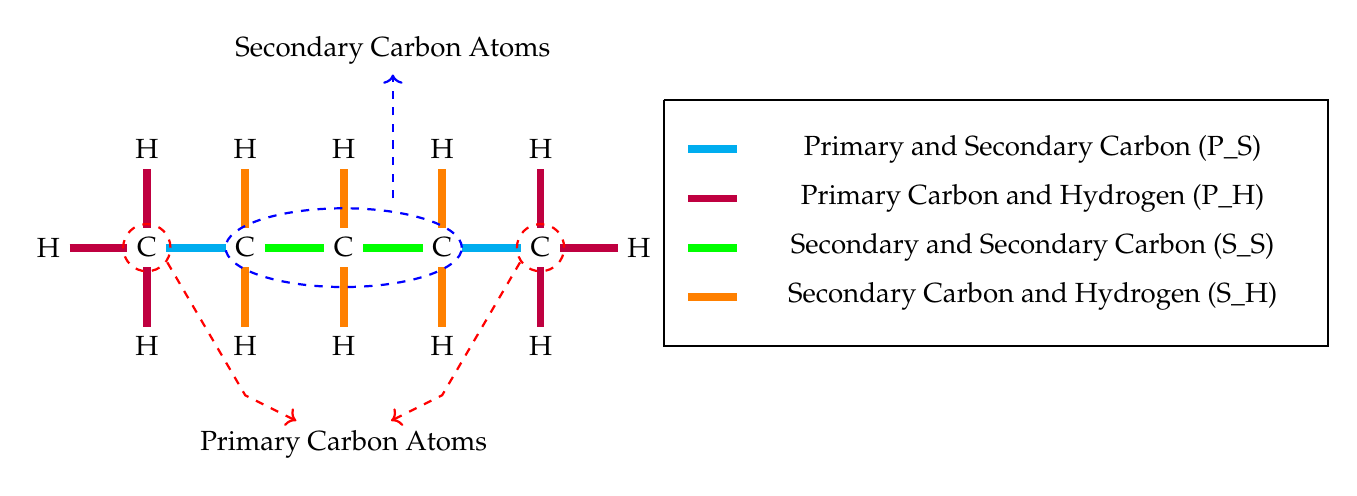
\begin{tikzpicture}[x=1.25cm,y=1.25cm]
								%Nodes Defined
								\node at (0,0) (nodeHstart) {H};
								\node at (1,0) (nodeC1) {C};
								\node at (1,1) (nodeC1H1) {H};
								\node at (1,-1) (nodeC1H-1) {H};
								\node at (2,0) (nodeC2) {C};
								\node at (2,1) (nodeC2H2) {H};
								\node at (2,-1) (nodeC2H-2) {H};
								\node at (3,0) (nodeC3) {C};
								\node at (3,1) (nodeC3H3) {H};
								\node at (3,-1) (nodeC3H-3) {H};
								\node at (4,0) (nodeC4) {C};
								\node at (4,1) (nodeC4H4) {H};
								\node at (4,-1) (nodeC4H-4) {H};
								\node at (5,0) (nodeC5) {C};
								\node at (5,1) (nodeC5H5) {H};
								\node at (5,-1) (nodeC5H-5) {H};
								\node at (6,0) (nodeHend) {H};
							
						%connecting nodes by drawing
					 \draw[line width=1mm,purple] (nodeHstart) -- (nodeC1);
					 \draw[line width=1mm,purple] (nodeC1) -- (nodeC1H1);
					 \draw[line width=1mm,purple] (nodeC1) -- (nodeC1H-1);
					 \draw[line width=1mm,cyan] (nodeC1) -- (nodeC2);
				  \draw[line width=1mm,orange] (nodeC2) -- (nodeC2H2);
				  \draw[line width=1mm,orange] (nodeC2) -- (nodeC2H-2);
					 \draw[line width=1mm,green] (nodeC2) -- (nodeC3);
				  \draw[line width=1mm,orange] (nodeC3) -- (nodeC3H3);
				  \draw[line width=1mm,orange] (nodeC3) -- (nodeC3H-3);
					 \draw[line width=1mm,green] (nodeC3) -- (nodeC4);
				  \draw[line width=1mm,orange] (nodeC4) -- (nodeC4H4);
				  \draw[line width=1mm,orange] (nodeC4) -- (nodeC4H-4);
					 \draw[line width=1mm,cyan] (nodeC4) -- (nodeC5);
				  \draw[line width=1mm,purple] (nodeC5) -- (nodeC5H5);
				  \draw[line width=1mm,purple] (nodeC5) -- (nodeC5H-5);
					 \draw[line width=1mm,purple] (nodeC5) -- (nodeHend);
					 
							 %Circle
							 \draw[red,thick,dashed] (1,0) circle (0.3cm);
 							 \draw[red,thick,dashed] (5,0) circle (0.3cm);
							\draw[blue,thick,dashed] (3,0) ellipse (1.5cm and 0.5cm);
							
							%circle node and arrow node
							\node at (1.15,-0.05) (StartCir){} ;
							\node at (3,-2) (ArrowTail){Primary Carbon Atoms};
							\node at (4.85,-0.05) (EndCir){};
							 %drawing
							 
							 \draw[red,thick,dashed,->] (StartCir) -- (2,-1.5) -- (ArrowTail);
							 \draw[red,thick,dashed,->] (EndCir) -- (4,-1.5) -- (ArrowTail);
							
							%circle node and arrow node Secondary carbon
							\node at (3.5,2) (endSec) {Secondary Carbon Atoms};
							\draw[blue,thick,dashed,->] (3.5,0.5) -- (endSec) ;
							
							%representing colours 
						\draw[line width=0.25mm] (6.25,1.5) --(13,1.5) -- (13,-1) -- (6.25,-1) -- (6.25,1.5) ;
						\draw[line width=1mm,cyan](6.5,1)--(7,1) ;
						\node at (10,1) (PS) {Primary and Secondary Carbon  (P\_S)};
						
						\draw[line width=1mm,purple](6.5,0.5)--(7,0.5) ;
						\node at (10,0.5) (PS) {Primary Carbon and Hydrogen (P\_H)};
						
						\draw[line width=1mm,green](6.5,0)--(7,0) ;
						\node at (10,0) (PS) {Secondary and Secondary Carbon (S\_S)};
						
						\draw[line width=1mm,orange](6.5,-0.5)--(7,-0.5) ;
						\node at (10,-0.5) (PS) {Secondary Carbon and Hydrogen (S\_H)};


							\end{tikzpicture}}
						\vspace{0.3cm}
							\caption{Different type of bonds in straight alkane (Pentane)}
							\label{fig:fuelbond}
							}
					     	}
						\end{figure}
							
							Bond information of fuel is obtained using SMILE (Simplified molecular-input line-entry system), which is method for computer to extract information and make it processable. It is based on molecular graph theory. SMILES follows certain rules to make entry of chemicals \cite{weininger1988smiles}. Chemical molecular structure are well defined by line entry system to acquire required information.
							
							RDKit \cite{rdkit} in python was used to extract the bond information. Using SMILES and RDKit, Mol-file was obtained. Mol-file gives information about Bond connections and orientation of bond in 3D space. By text processing of Mol-Block(file) bond information was extracted. 
							
						 It is clear from the figure-\ref{fig:fuelbond} that, straight chain alkane (for carbon chain $>$ 2)contains 4 different type of bonds. Ethane is only fuel in which primary-primary carbon bond exist so that fuel is excluded from the analysis. Bond details were extracted from the Mol-file. Different type of bond detail are used as parameters in the dataset. Using all the obtain information final dataset given in table-\ref{table:dataset}. 
						 
						 \begin{table}[h]
						 	\small{\scalebox{0.75}{
						 	\begin{tabular}{|l|l|l|l|l|l|l|l|l|l|l|l|}
						 		\hline
						 		Fuel & T(K) & T\_Error(\%) & P(atm) & P\_Error(\%) & Fuel(\%) & Oxygen(\%) & P\_S & S\_S & P\_H & S\_H & Time($\mu s$) \\ \hline
						 		CCC & 1376 & $\pm$1 & 1.19 & $\pm$1 & 4 & 20 & 2 & 0 & 6 & 2 & 357 \\ \hline
						 		CCCC & 1409 & $\pm$1 & 1.17 & $\pm$1 & 1 & 6.5 & 2 & 1 & 6 & 4 & 390 \\ \hline
						 		CCCCC & 1395 & $\pm$0.7 & 3.47 & $\pm$1 & 0.5 & 4 & 2 & 2 & 6 & 6 & 316 \\ \hline
						 		CCCCCC & 1273 & $\pm$0.7 & 3.32 & $\pm$1 & 0.42 & 4 & 2 & 3 & 6 & 8 & 1046 \\ \hline
						 		CCCCCCC & 1378 & $\pm$1 & 2.326 & $\pm$1 & 0.03 & 0.33 & 2 & 4 & 6 & 10 & 1330 \\ \hline
						 		CCCCCCCC & 1289 & $\pm$0.7 & 2.01 & $\pm$1 & 0.32 & 4 & 2 & 5 & 6 & 12 & 1198 \\ \hline
						 		CCCCCCCCC & 1107 & $\pm$0.7 & 14.8 & $\pm$1 & 0.4 & 4 & 2 & 6 & 6 & 14 & 965 \\ \hline
						 		CCCCCCCCCC & 1081 & $\pm$2 & 5.14 & $\pm$9.6 & 1.44 & 21 & 2 & 7 & 6 & 16 & 1696 \\ \hline
						 		CCCCCCCCCCCC & 1045 & $\pm$1 & 6.71 & $\pm$9.3 & 0.6098 & 21 & 2 & 9 & 6 & 20 & 2753 \\ \hline
						 		CCCCCCCCCCCCCCCC & 1181 & $\pm$2 & 2.13 & $\pm$1 & 0.1776 & 4 & 2 & 13 & 6 & 28 & 5536 \\ \hline
						 	\end{tabular}
						 	\label{key}
						 }}
						 \vspace{0.3cm}
						 	\caption{Fuel dataset made after obtaining bond information. Uncertainty in parameter is replace by least least available value in-case not reported. Fuel is represented using SMILE. T$\_$Error($\%$) and P$\_$Error($\%$)  represents uncertainty in measurement of temperature and pressure respectively. Bond notation are same as mentioned in figure-\ref{fig:fuelbond}    }
						 	\label{table:dataset}
						 \end{table}
					
					\section{Data Clustering and Analysis:}
					  The obtained ignition delay has wide range of conditions for temperature, pressure, Fuel and Oxygen Mole fraction for variety of fuel. Multi-linear regression of dataset without any treatment gives poor coefficient of determination $\rm R^2$ = 0.79  which indicates that dataset has to divide based on certain pattern.
					  
					Ignition delay data of Alkanes have 8 parameters. Visualization of such data points in higher dimension is not possible  whereas  straightforward in less dimensions. Weiqi et al. has divided the dataset based on the turnover states to revels distinct thermodynamic and kinetic property under different pressure \cite{controlling}. To develop IDT correlation for Hydrogen/air mixture, Zhao et al. \cite{zhao2011correlations} has divided the dataset into six sub domains based on high, intermediate and low pressure along with low and High temperature range. Such finding motivates to divide the dataset into sub parts.
					
					Due to recent advancement in machine learning, it is possible to unveil concealed pattern of n-Dimensional data using different clustering technique, which is one of the famous unsupervised learning technique for unlabelled data. Out of many available algorithm, K-Means is famous and  preferred partition based algorithm. It performs better in terms accuracy and execution time compared to other algorithm\cite{clustering}. K-Means algorithm generates K centroids and minimizes the distance between cluster centroids and data-points for given number of clusters.\\
					
					K-Means Algorithm:
					\begin{itemize}
						\item Consider the data points $x_i= {x_1, x_2, x_3, ... , x_n} \in \mathbf {R}^d $  has j features. $\mu_i \in \mathbf {R}^d$ denotes number of clusters and $q_1, ... ,q_n$ $\in$ $\{1, ... , K\}$ denotes points assigned to the centroid. Such that the sum of distances 
						 is minimized within cluster which is defined as,
						\begin{equation}
 E (\mu_1, \mu_2,.., \mu_K, q_1, q_2, ... ,q_n) =  \sum_{i=1}^{k} ||x_i - \mu_{q_i} ||^p_P
						\end{equation}
						where p denotes the norm.
						\item {steps:} 
						\begin{enumerate}
							\item Randomly select the K initial cluster centroid.
							\item Assign the data points to nearest cluster 
							\item Recompute the  cluster based current data members of associated cluster
							\item Repeat the procedure till convergence criteria not met or clusters are not moving (Go to step:2) 
						\end{enumerate}
					\end{itemize} 
					
					K-Means algorithm is used from scikit-learn library. Which computes the clusters using  Elkan's algorithm \cite{scikit-learn}. K-Means is useful method when number of clusters are known. But for the case of IDT, number of clusters are unkowns. To find out optimal number of clusters, elbow method is used along with silhouette criteria.
					
					Elbow method calculates within-cluster sum of squared error (WCSSE) for given k cluster by equation-\ref{eq:WCSSE}.  The K-value for which WCSSE starts declining, gives the optimized number of clusters as   it minimizes the WCSSE.
					\begin{equation}\label{eq:WCSSE}
						WCSSE = \sum_{i=1}^{n} \sum_{x \in S_i} ||x_i - \mu_i||^2
					\end{equation}
					
					 For ignition delay data, WCSSE is calculated for 2 to 11 number of clusters. Apart from ethane, all available data has been used to generate the clusters.  From fig-\ref{fig:WCSSE}, it was observed that elbow(sharp slope) was generated around K=3 or K=4. The obtained result from fig-\ref{eq:WCSSE} is quite ambiguous to analyse. To have more robust decision Silhouette criteria was needed along with elbow method.
					 	 
					 	 \begin{figure}[H]\label{fig:cluster}
					 	 	\subfigure[Elbow Method Result - Within-cluster sum of squared error(WCSSE) vs Number of cluster to decide the optimum number of cluster for K-Means]{\label{fig:WCSSE}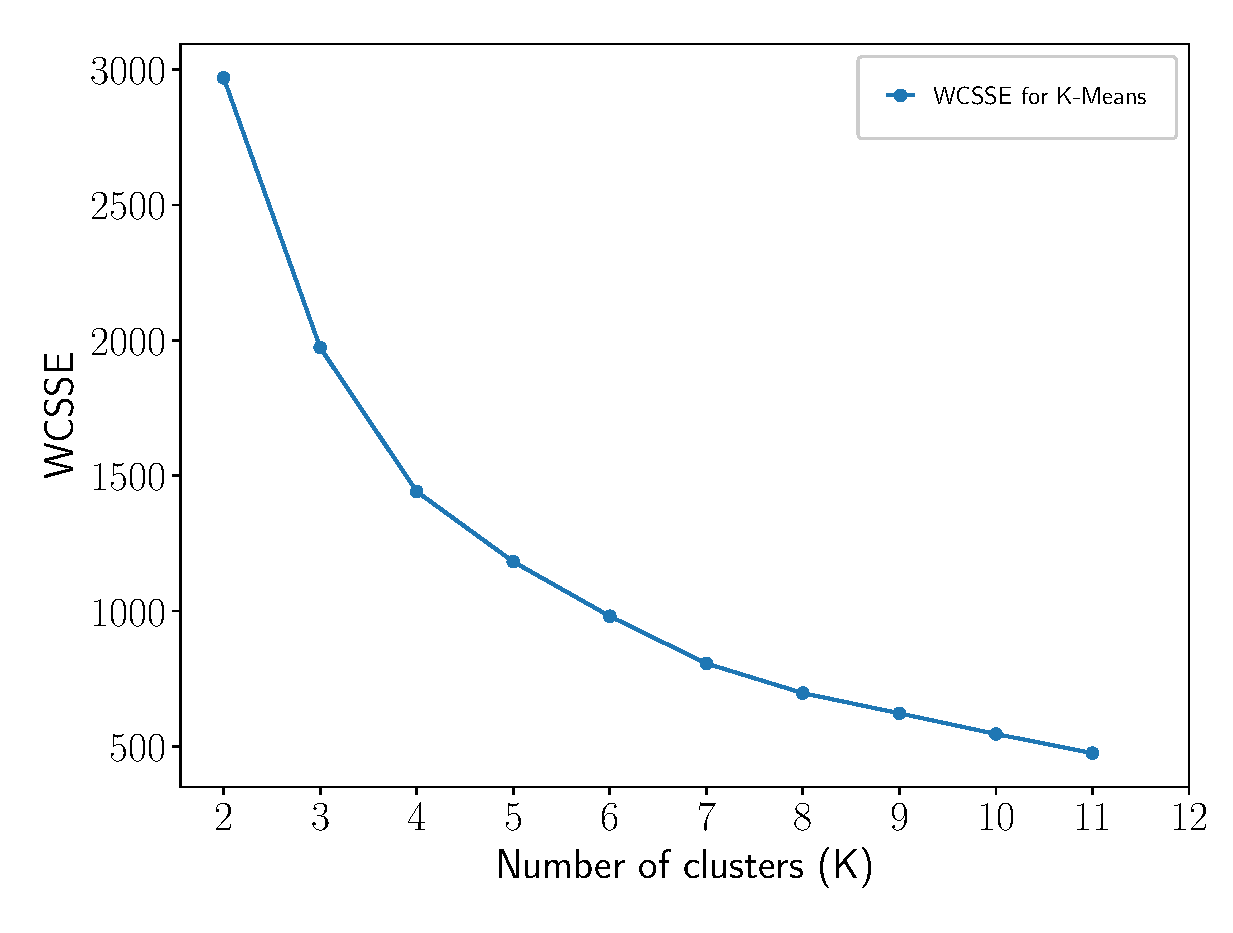
\includegraphics[scale=0.395]{WCSSE.eps}}
					 	 	\hspace{0.25cm}
					 	 	\subfigure[Silhouette Score vs Number of cluster for different clustering technique  ]{\label{fig:diff_cluster}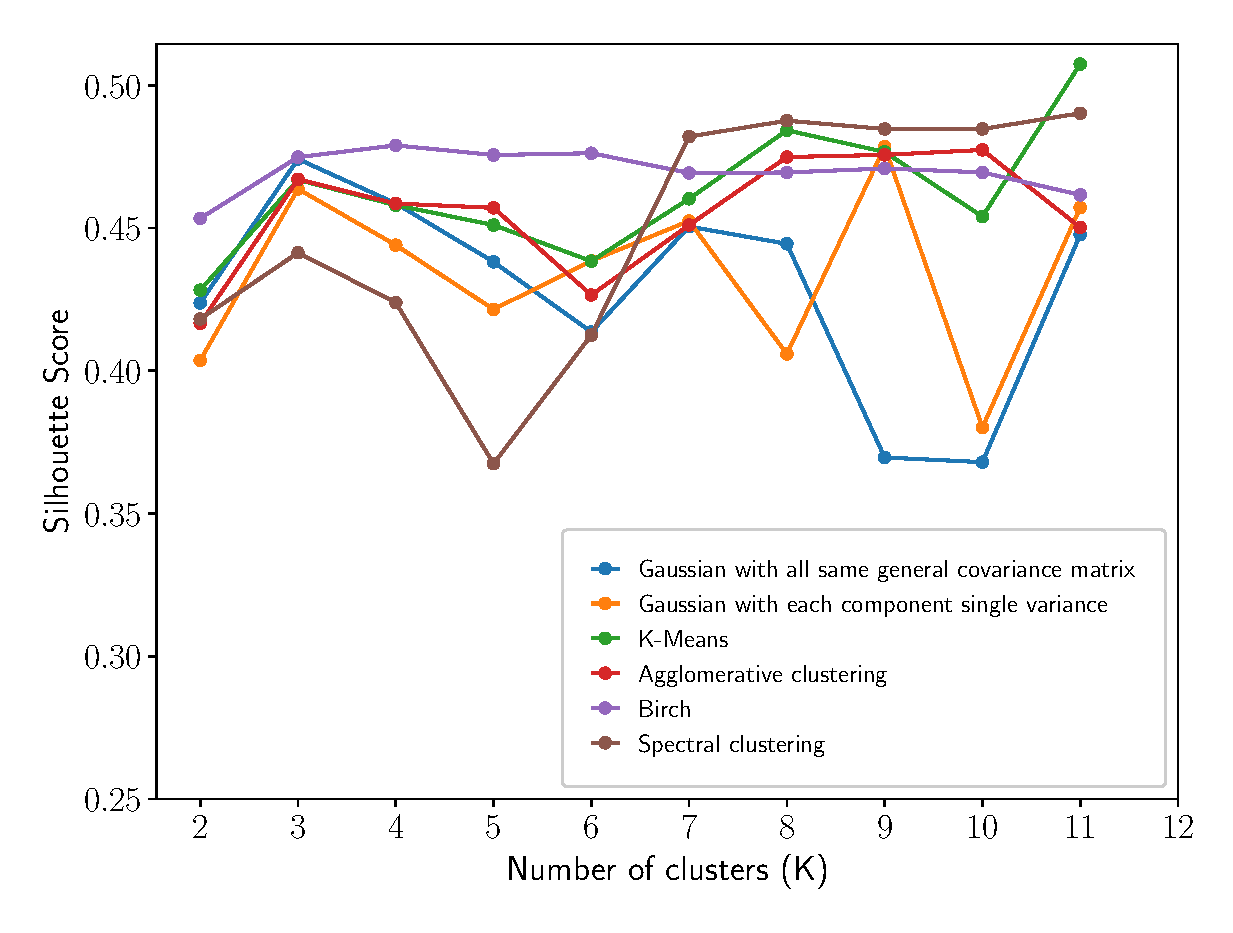
\includegraphics[scale=0.360]{silhouette.eps}}
					 	 	\caption{Criteria to decide the number of clusters for all fuel components}
					 	 \end{figure}
					 	 \vspace{0.5cm}					 	 
					 
				
					 
					 
\textbf{Silhouette Score Calculation:}\cite{Silhouettes} \cite{recovering}
					 \begin{itemize}
					 	\item Data were divided into K-clusters
					 	\item Each data point $x_i$ is assigned to cluster $C_{k}$ such that ,$\forall x $ $x_i \in C_k$
					 	\item Silhouette criteria measures the relative separation distance between points in same cluster to other clusters. Mean distance \textbf{within cluster} from point i to other points were measured by,
					 	\begin{equation}
								a(i) = \frac{1}{|C_i| - 1} \sum_{j \in C_i, i \neq j} d(i, j)
					 	\end{equation}
					 	where, $d(i,j)$ is the distance between data points  i and j in the cluster $ C_i$. Numerator contains $|C_i|-  1$ as $d(i,i)$ is excluded. In summary, $a(i)$ shows  how well data point i is assigned to its cluster. Smaller value is expected for proper assignment.
					 	\item Mean distance between point i in cluster C to \textbf{points in other cluster} were measured by following equation:
					 	
					 	\begin{equation}
								b(i) = \min_{k \neq i} \frac{1}{|C_k|} \sum_{j \in C_k} d(i, j)
					 	\end{equation}
					 	Use of min operator on cluster k shows that out of all value of different cluster, minimum value is used for calculation of $b(i)$ which is nearest neighbouring cluster to that specific point-i. Large value of $b(i)$ suggest that point-i does not properly matches with neighbouring cluster.
					 	\item Silhouette for points-i is defined as,
					 	
					 	\begin{equation}
				 		s(i) =
						 	\begin{cases} 
					 	 \frac{b(i) - a(i)}{\max\{a(i),b(i)\}} 	 & |C_i|  > 1 \\ 
						 	0 & |C_i|  = 1 \\
						 	\end{cases}				 			
					 	\end{equation}
					 	which is also defined as,
					 	\begin{equation}
								s(i) =
								\begin{cases} 
								 1- \frac{a(i)}{b(i)} 	 & if \hspace{0.25cm} |a_i|  < |b_i|  \\ 
								0 & if \hspace{0.25cm} |a_i|  = |b_i|  \\ 
								\frac{b(i)}{a(i)} - 1  	 & if \hspace{0.25cm} |a_i|  > |b_i|  \end{cases}		 
					 	\end{equation}
					 \item $s(i)$ was calculated for all the points. The average value $s(i)$ in the cluster shows how tightly all point are assembled in the cluster. Mean $s(i)$ of of whole dataset shows how properly data points forms the group.
					 	 
					 \end{itemize} 
					 
			 	 
					 Silhouette analysis is useful for each data point to measure the distance between the clusters they belong and other neighbouring clusters. Silhouette Score varies from -1 to 1 in which 1 is ideal which shows that object are well separated and -1 shows improper clustering. To calculate Silhouette Score, sklearn.metrics.silhouette_score function is utilized.
					 
					 For IDT dataset, Silhouette analysis has been  done using different clustering algorithm. First drop in result was observed at cluster K=3 for clustering techniques which emphasis that data should be divided into three partition. IDT dataset-\ref{fuel_data_summary} has large variation in data points. Observed result is quite sensitive to type of fuel, conditions affecting to IDT and number of data points. For verification of technique and to check biasness in the result, silhouette analysis has been done on fuel which has more than 100 data points. From table-\ref{fuel_data_summary}, it observed that propane, heptane and dodecane satisfies that criteria. Those fuel also covers wide of range of conditions. The observed result given in fig-\ref{fig:WCSSE_3fuel} and fig-\ref{fig:diff_cluster_3fuel} shows similar trend obtained in case if 'all fuel' - \ref{fig:diff_cluster} \ref{fig:WCSSE}. It clear from the fig-\ref{fig:diff_cluster_3fuel} that number of cluster required for dataset of propane, heptane and dodecane is also 3.
						\begin{figure}[H]\label{fig:3fuelcluster}
							\subfigure[Elbow Method Result: Within-cluster sum of squared error(WCSSE) vs Number of cluster for K-Means using data points of Propane, Heptane and Dodecane Fuel ]{\label{fig:WCSSE_3fuel}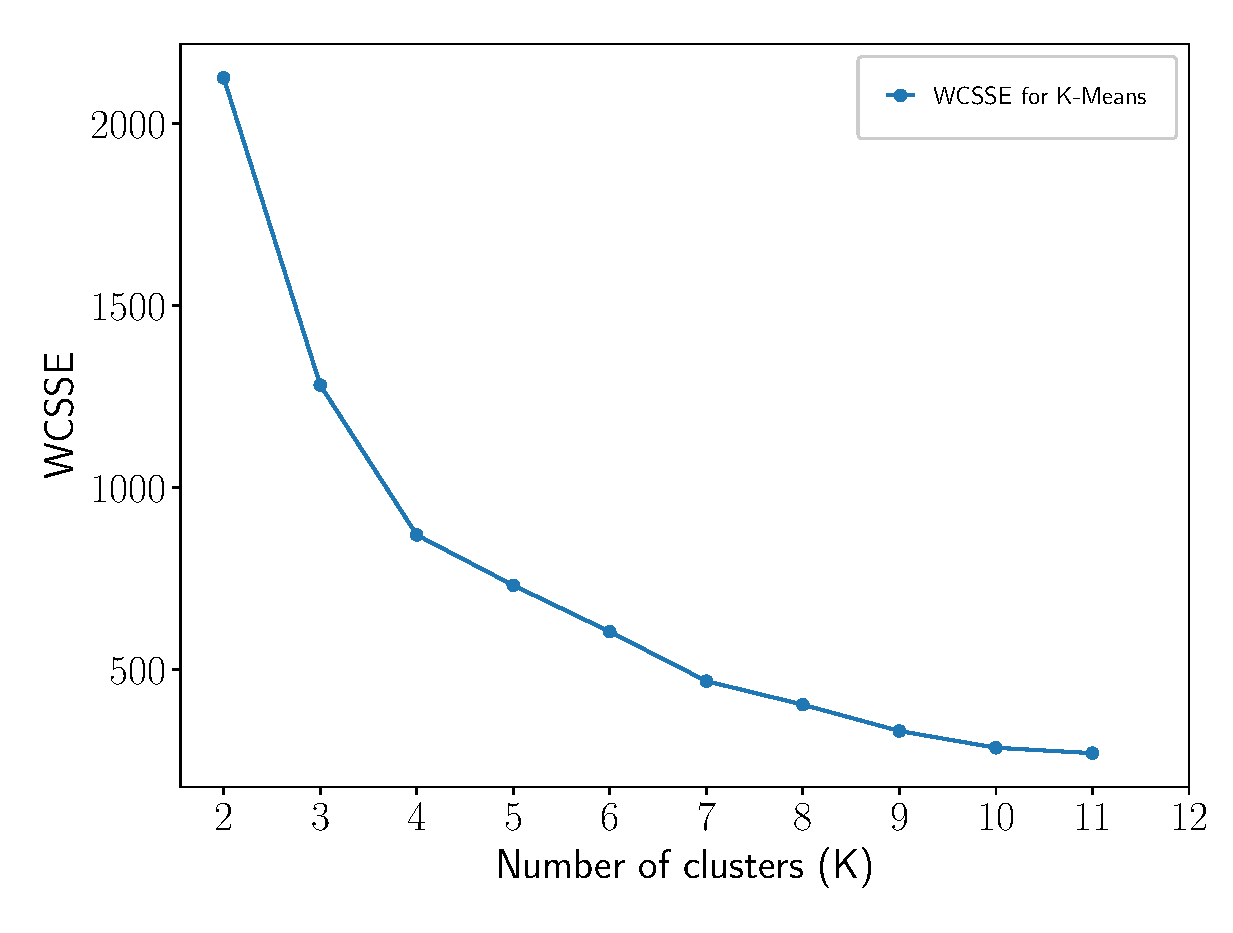
\includegraphics[scale=0.365]{Highest_WCSSE.eps}}
							\hspace{0.25cm}
							\subfigure[Result of Silhouette Score vs Number of cluster for different clustering technique using data points of Propane, Heptane and Dodecane  ]{\label{fig:diff_cluster_3fuel}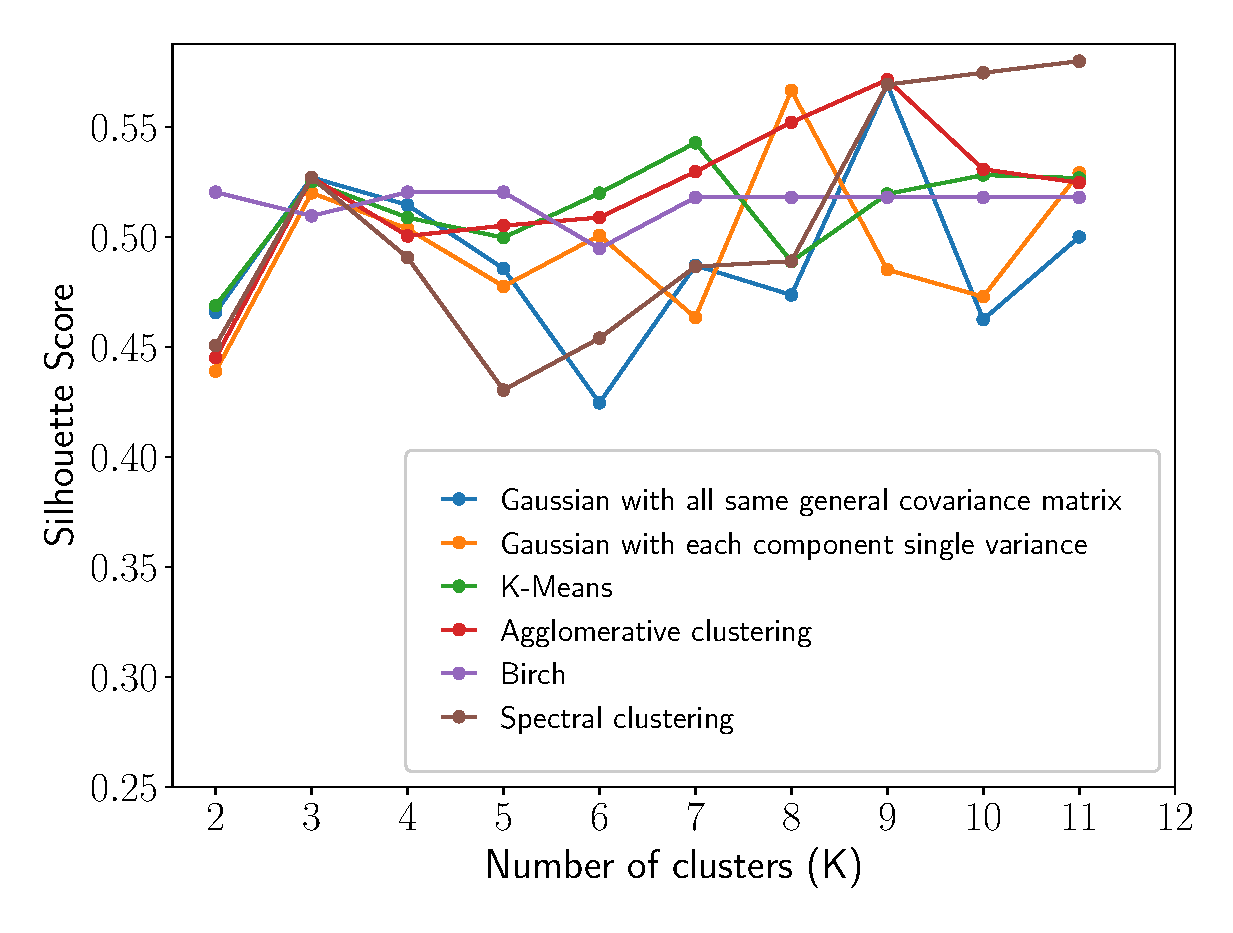
\includegraphics[scale=0.365]{Highest_silhouette.eps}}
							\caption{Criteria to decide the number of clusters obtained using Propane, Heptane and Dodecane}
						\end{figure}
						
						\begin{figure}[H]\label{fig:propanecluster}
							\subfigure[Elbow Method Result: Within-cluster sum of squared error(WCSSE) vs Number of cluster for K-Means using data points of Propane ]{\label{fig:WCSSE_prorane}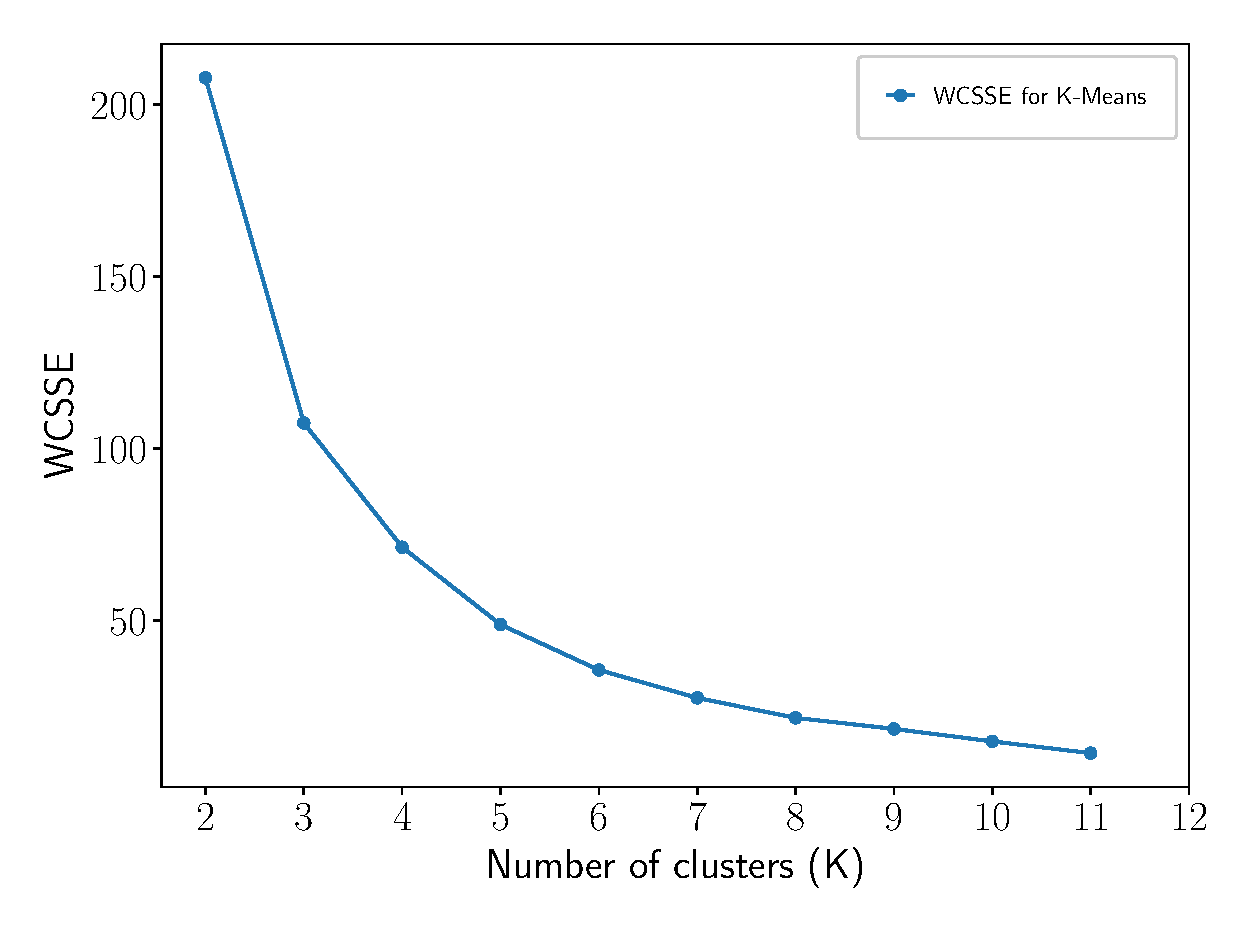
\includegraphics[scale=0.365]{only_propane_WCSSE.eps}}
							\hspace{0.25cm}
							\subfigure[Result of Silhouette Score vs Number of cluster for different clustering technique using data points of Propane ]{\label{fig:diff_cluster_propane}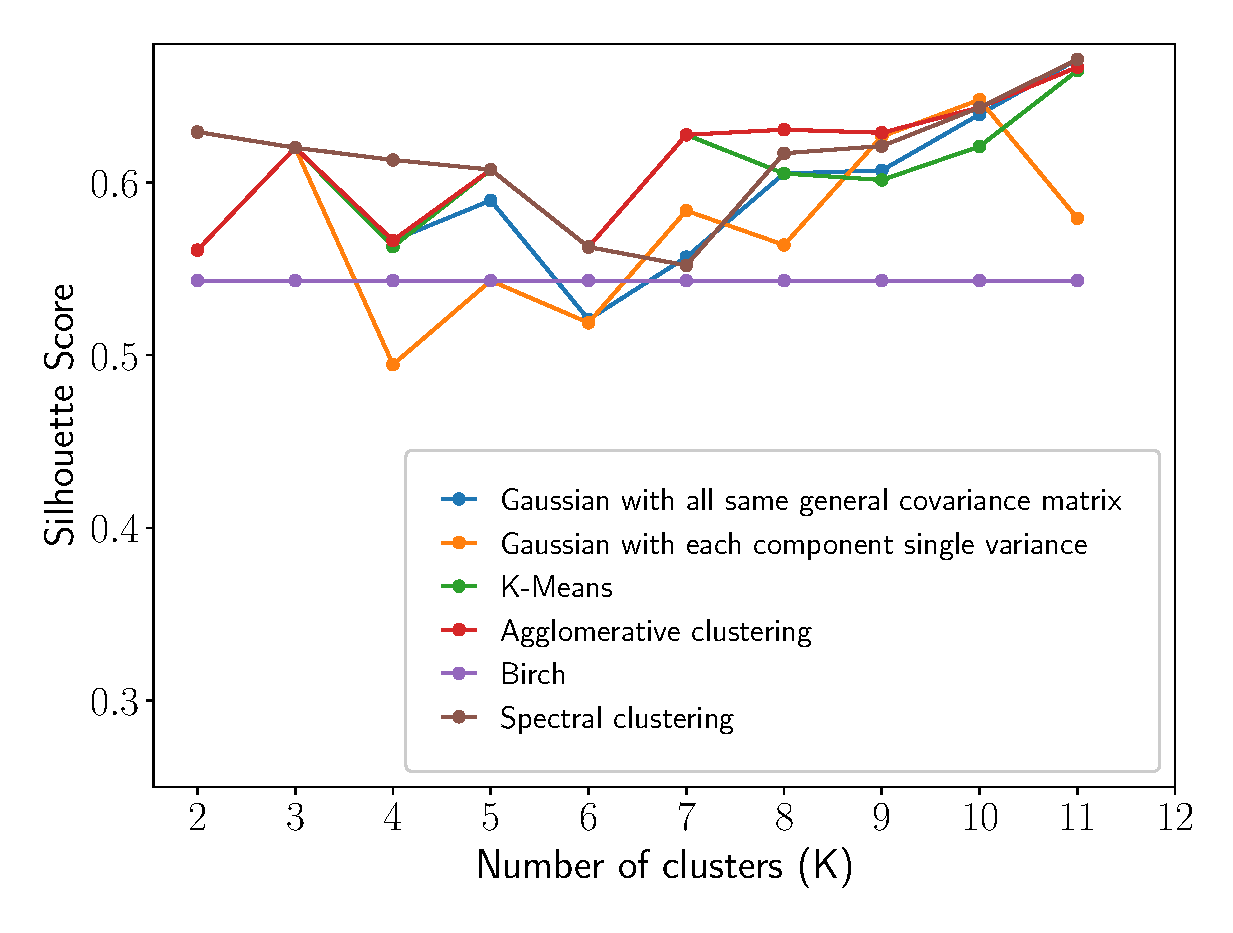
\includegraphics[scale=0.365]{only_propane_silhouette.eps}}
							\caption{Criteria to decide the number of clusters obtained using Propane}
						\end{figure}
						
						Similar result was also observed in case of individual fuel dataset of Propane, Heptane as given in figure-\ref{fig:diff_cluster_propane},\ref{fig:diff_cluster_heptane} which also agrees with expected trend. For propane and heptane observation  matches with expected trend whereas in case of heptane -\ref{fig:diff_cluster_dode}, it suggest to divide the dataset into two sub-dataset as Dodecane data points has limited range of physical conditions. Dodecane data, in table-\ref{fuel_data_summary} shows that, compared to heptane and propane data is limited by pressure at 33.7 whereas, propane and heptane has pressure around 60 atm. Similar observation is also made in equivalence ratio.						  
						
						Silhouette score obtained in all the cases is above 0.4 which emphasis that data points are grouped by certain parameters. At a same time, clustering value is far away from 1 which means that they do not generate perfect cluster and data are quite separated  which is useful information for regression analysis. 
								\begin{figure}[H]\label{fig:heptanecluster}
									\subfigure[Elbow Method Result: Within-cluster sum of squared error(WCSSE) vs Number of cluster for K-Means using data points of Heptane ]{\label{fig:WCSSE_heptane}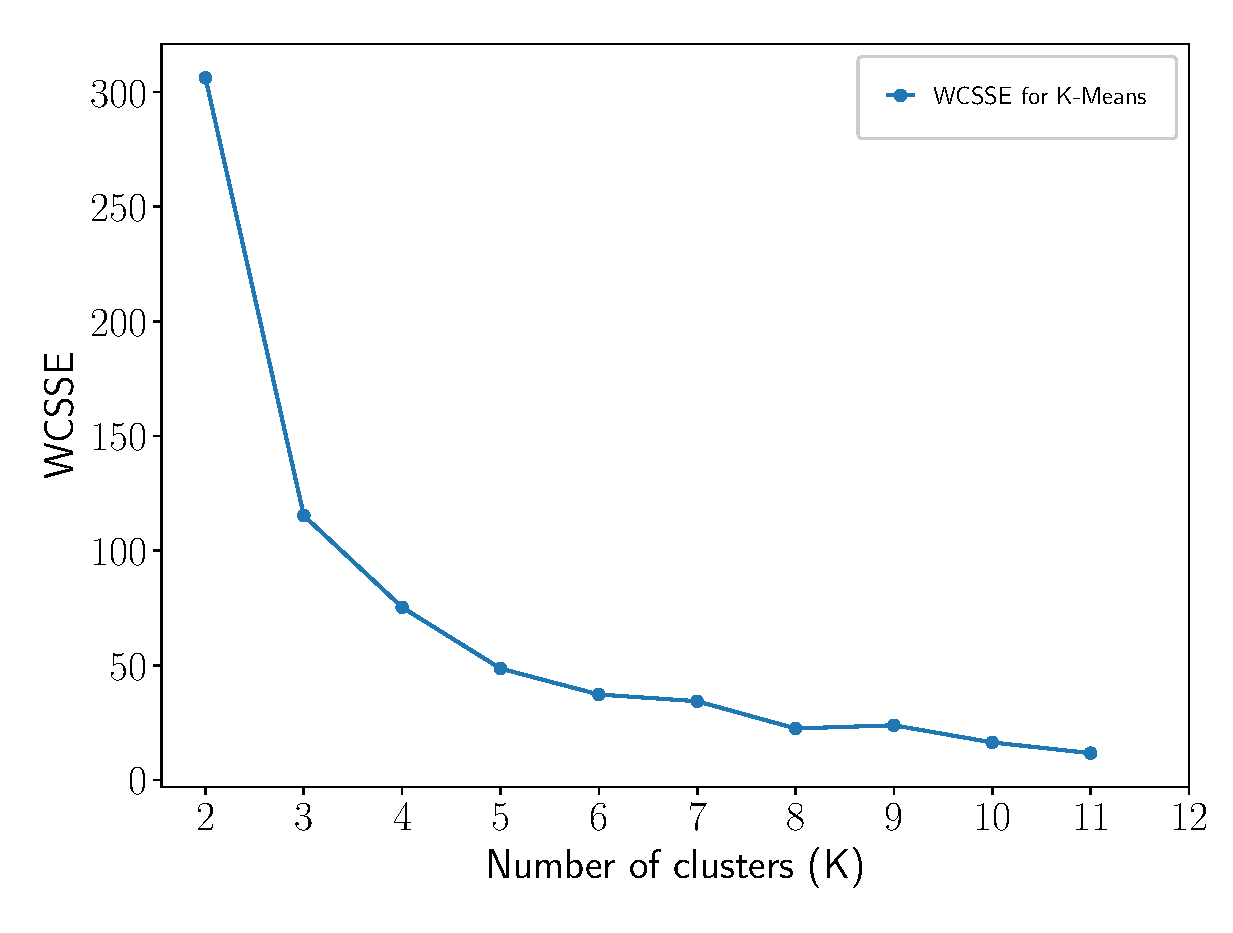
\includegraphics[scale=0.365]{only_Heptane_WCSSE.eps}}
									\hspace{0.25cm}
									\subfigure[Result of Silhouette Score vs Number of cluster for different clustering technique using data points of Heptane]{\label{fig:diff_cluster_heptane}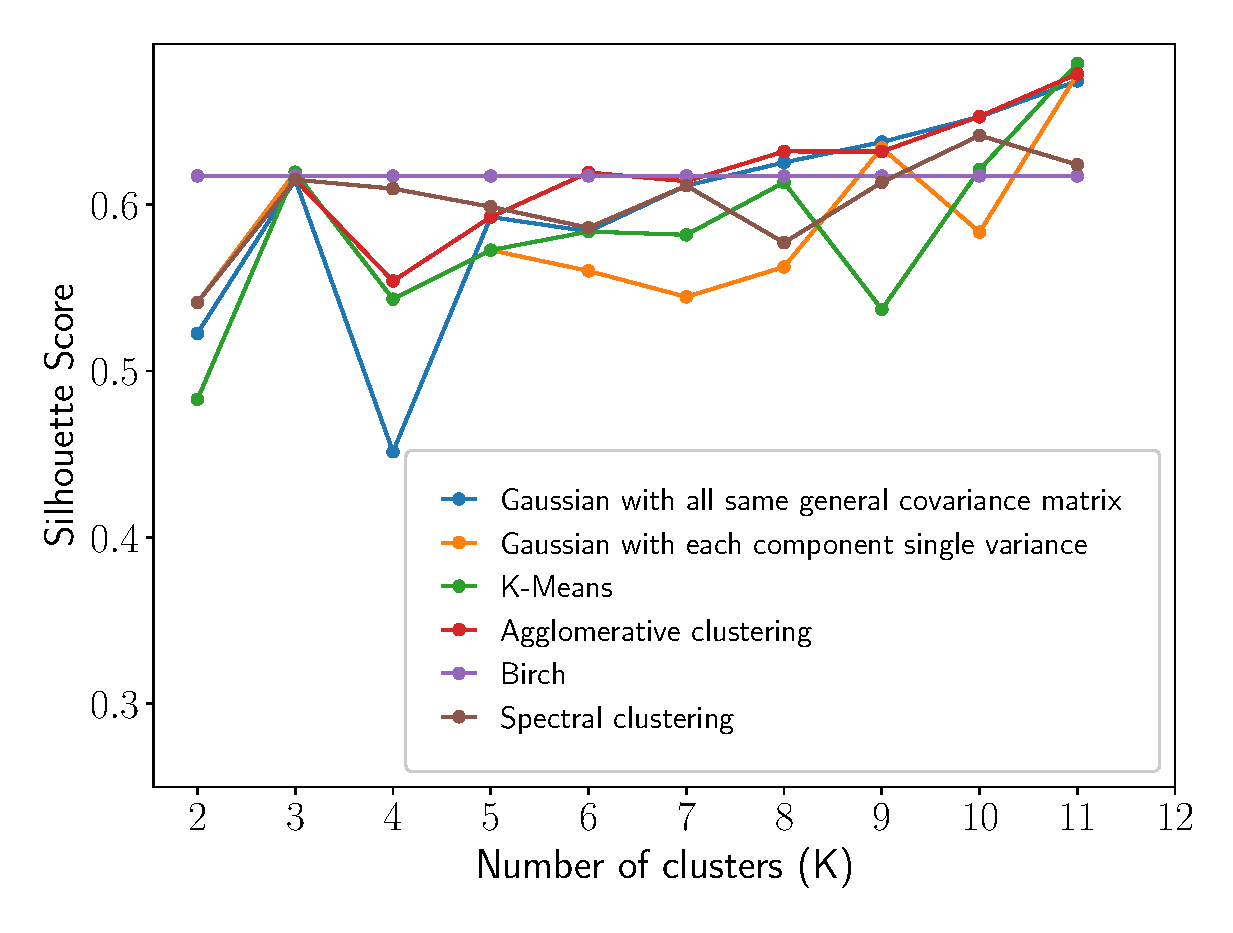
\includegraphics[scale=0.365]{only_Heptane_silhouette.eps}}
									\caption{Criteria to decide the number of clusters obtained using Heptane}
								\end{figure}
									\begin{figure}[H]\label{fig:dodecanecluster}
										\subfigure[Elbow Method Result: Within-cluster sum of squared error(WCSSE) vs Number of cluster for K-Means using data points of Dodecane ]{\label{fig:WCSSE_dode}\includegraphics[scale=0.365]{only_dodecane_WCSSE.eps}}
										\hspace{0.25cm}
										\subfigure[Result of Silhouette Score vs Number of cluster for different clustering technique using data points of Dodecane  ]{\label{fig:diff_cluster_dode}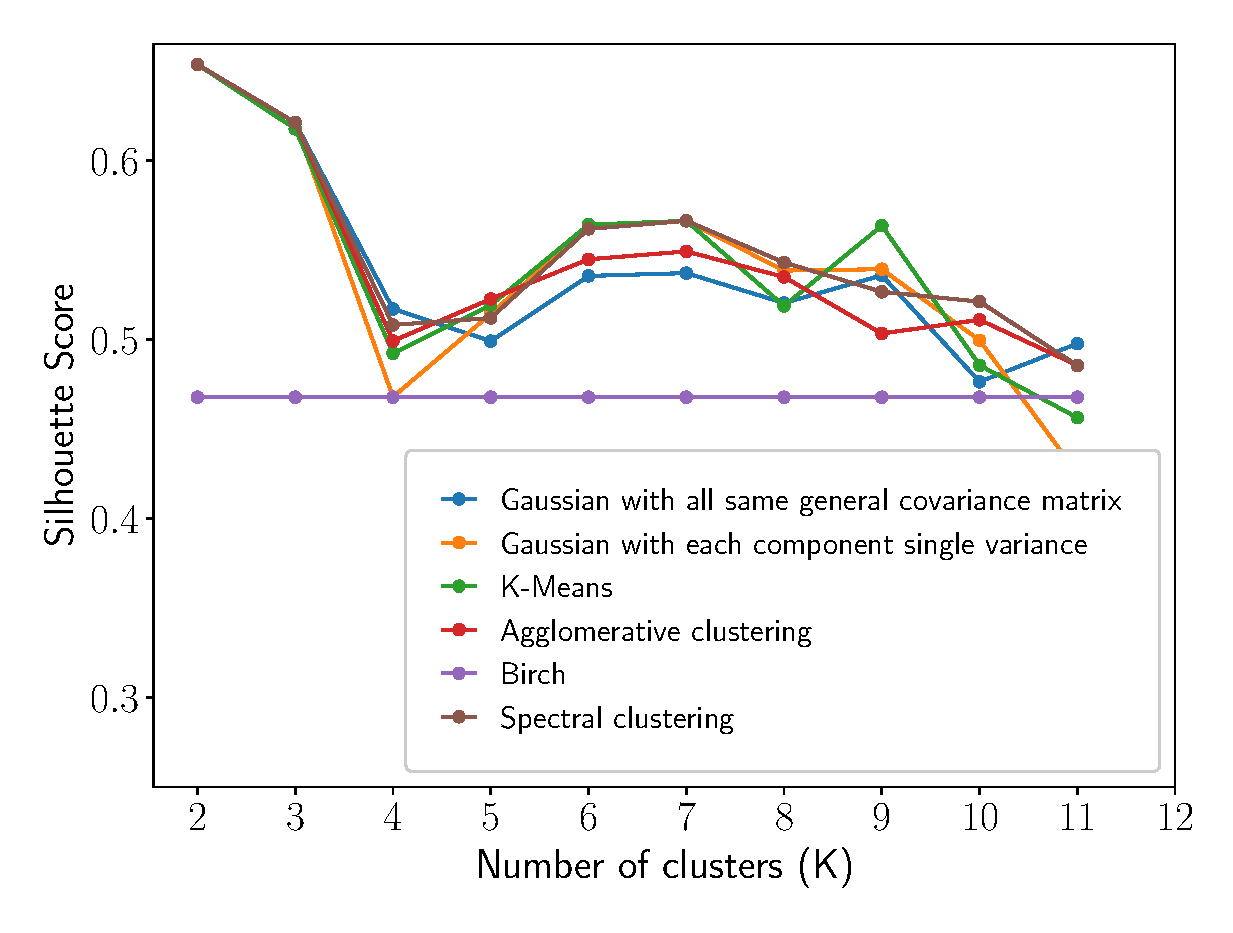
\includegraphics[scale=0.365]{only_dodecane_silhouette.eps}}
										\caption{Criteria to decide the number of clusters obtained using Dodecane}
									\end{figure}
						\subsection{Principal Component Analysis (PCA) of Dataset}  
								Principal component analysis is useful for dimensionality reduction and for analysis of major component of the data. For given data, PCA find out major eigen values and eigen vector. Principle components obtained using full SVD solver showed that, data has 6 major eigen values and other two are near to 0. For (616, 8) size of dataset obtained variation in principal components(Eigen values) are obtained as below:
								\[\begin{matrix}\label{mat:eigenvalues}
								    4.80958553e+00 & 2.55919622e+00 & 1.15728172e+00 & 9.98961156e-02 \\
								    2.33198384e-02 & 1.68372670e-04 & 2.93116344e-32 &1.18120890e-33
								\end{matrix}\]							
								From six eigenvalues it is clear that, it has major three principal eigen values and out of rest, other three are smaller eigen values. so, it is possible to visualize the major variation in data and clustering in the 3-Dimensions.
								To visualize the clustering of data in 3D, K-Means along with PCA was implemented. Obtained result are given in fig-\ref{fig:pca2d} and -\ref{fig:pca3d}. Obtained result also supports the the criteria to divide the dataset into 3 component.								
								\begin{figure}[h]\label{fig:pca}
									\subfigure[Major 2 components ontained by PCA and K-Menas on that major 2 components  ]{\label{fig:pca2d}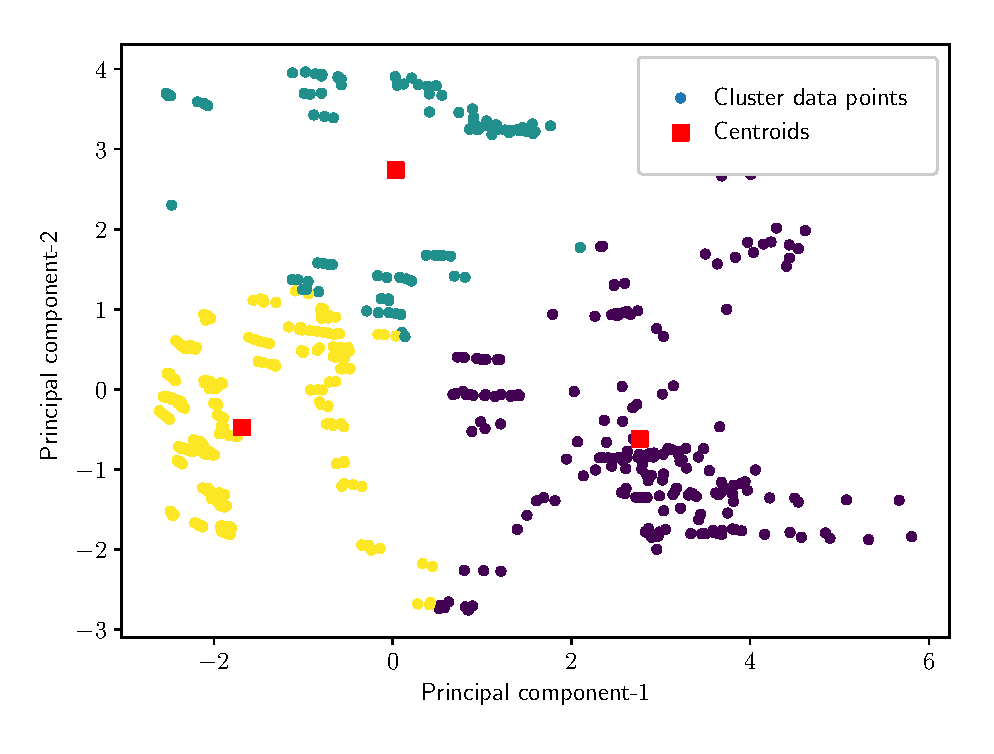
\includegraphics[scale=0.45]{PCA_2D.eps}}
									\hspace{0.25cm}
									\subfigure[Major 3 components ontained by PCA and K-Menas on that major 2 components   ]{\label{fig:pca3d}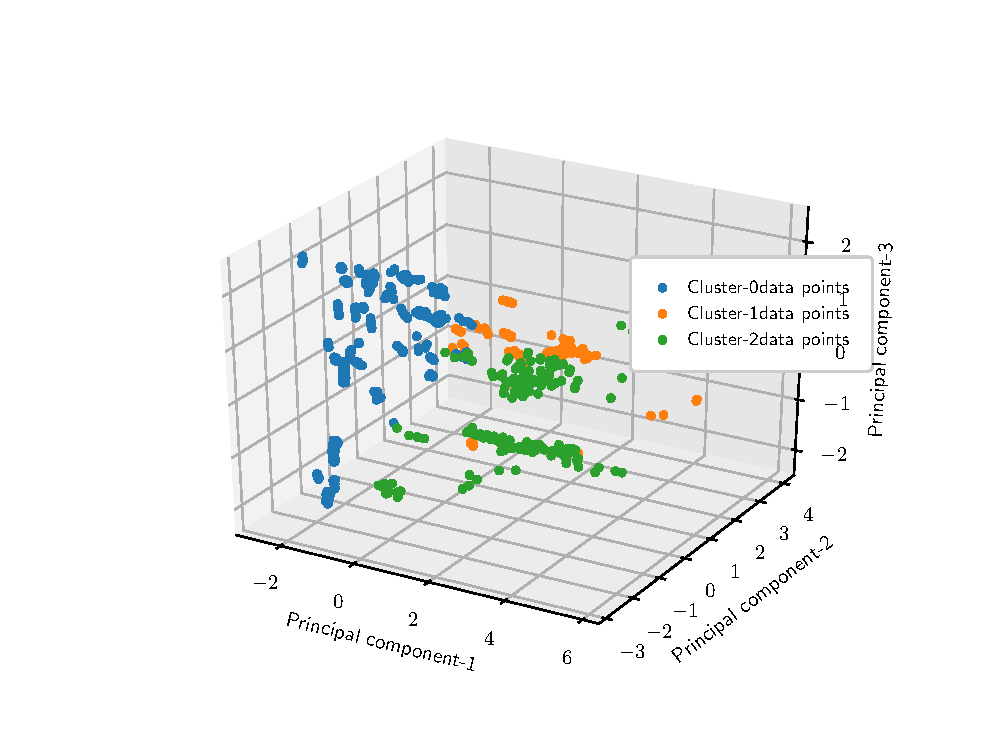
\includegraphics[scale=0.55]{PCA_3D.eps}}
									\caption{PCA and K-Means of all the fuels }
								\end{figure}
								
					\subsection{Analysis of classified sub-dataset}
					Main dataset is divide into the three sub-dataset using silhouette criteria and K-Means clustering algorithm. By analysing the sub-dataset, obtained observations are discussed here.
					\subsubsection{Subdataset-I}
							
						It contains 331 data points. Mostly short and middle level alkanes at high pressure and temperature are part of this dataset. Certain data points at low temperate and high pressure are also part this set i.e. propane at 950K and 21.4 atm.
						% Please add the following required packages to your document preamble:
						% \usepackage{multirow}
						\begin{table}[H]
						\tiny \centering	\begin{tabular}{cccccccc}
							    \hline
								\multicolumn{1}{|c|}{Fuel} & \multicolumn{1}{l|}{} & \multicolumn{1}{c|}{\begin{tabular}[c]{@{}c@{}}Temperature\\ (K)\end{tabular}} & \multicolumn{1}{c|}{\begin{tabular}[c]{@{}c@{}}Pressure\\ (atm)\end{tabular}} & \multicolumn{1}{c|}{\begin{tabular}[c]{@{}c@{}}Fuel\\ Mole\\ \\ Fraction\\ (\%)\end{tabular}} & \multicolumn{1}{c|}{\begin{tabular}[c]{@{}c@{}}Oxygen \\ Mole \\ \\ Fraction\\ (\%)\end{tabular}} & \multicolumn{1}{c|}{\begin{tabular}[c]{@{}c@{}}Equivalence\\ Ratio\end{tabular}} & \multicolumn{1}{c|}{\begin{tabular}[c]{@{}c@{}}Data\\ Points\end{tabular}} \\ \hline
								\multicolumn{1}{|c|}{\multirow{2}{*}{\begin{tabular}[c]{@{}c@{}} Propane\end{tabular}}} & \multicolumn{1}{c|}{max} & \multicolumn{1}{c|}{1841} & \multicolumn{1}{c|}{67.8} & \multicolumn{1}{c|}{4} & \multicolumn{1}{c|}{20} & \multicolumn{1}{c|}{5} & \multicolumn{1}{c|}{\multirow{2}{*}{169}} \\ \cline{2-7}
								\multicolumn{1}{|c|}{} & \multicolumn{1}{c|}{min} & \multicolumn{1}{c|}{950} & \multicolumn{1}{c|}{1.12} & \multicolumn{1}{c|}{0.15} & \multicolumn{1}{c|}{0.75} & \multicolumn{1}{c|}{0.5} & \multicolumn{1}{c|}{} \\ \hline
								\multicolumn{1}{|c|}{\multirow{2}{*}{\begin{tabular}[c]{@{}c@{}} Butane\end{tabular}}} & \multicolumn{1}{c|}{max} & \multicolumn{1}{c|}{1761} & \multicolumn{1}{c|}{5.5} & \multicolumn{1}{c|}{2} & \multicolumn{1}{c|}{13} & \multicolumn{1}{c|}{2} & \multicolumn{1}{c|}{\multirow{2}{*}{55}} \\ \cline{2-7}
								\multicolumn{1}{|c|}{} & \multicolumn{1}{c|}{min} & \multicolumn{1}{c|}{1230} & \multicolumn{1}{c|}{1.03} & \multicolumn{1}{c|}{0.5} & \multicolumn{1}{c|}{3.25} & \multicolumn{1}{c|}{0.5} & \multicolumn{1}{c|}{} \\ \hline
								\multicolumn{1}{|c|}{\multirow{2}{*}{\begin{tabular}[c]{@{}c@{}} Pentane\end{tabular}}} & \multicolumn{1}{c|}{max} & \multicolumn{1}{c|}{1533} & \multicolumn{1}{c|}{3.75} & \multicolumn{1}{c|}{0.5} & \multicolumn{1}{c|}{4} & \multicolumn{1}{c|}{1} & \multicolumn{1}{c|}{\multirow{2}{*}{15}} \\ \cline{2-7}
								\multicolumn{1}{|c|}{} & \multicolumn{1}{c|}{min} & \multicolumn{1}{c|}{1261} & \multicolumn{1}{c|}{1.62} & \multicolumn{1}{c|}{0.25} & \multicolumn{1}{c|}{4} & \multicolumn{1}{c|}{0.5} & \multicolumn{1}{c|}{} \\ \hline
								\multicolumn{1}{|c|}{\multirow{2}{*}{\begin{tabular}[c]{@{}c@{}} Hexane\end{tabular}}} & \multicolumn{1}{c|}{max} & \multicolumn{1}{c|}{1475} & \multicolumn{1}{c|}{3.6} & \multicolumn{1}{c|}{0.42} & \multicolumn{1}{c|}{4} & \multicolumn{1}{c|}{1} & \multicolumn{1}{c|}{\multirow{2}{*}{16}} \\ \cline{2-7}
								\multicolumn{1}{|c|}{} & \multicolumn{1}{c|}{min} & \multicolumn{1}{c|}{1237} & \multicolumn{1}{c|}{1.67} & \multicolumn{1}{c|}{0.21} & \multicolumn{1}{c|}{4} & \multicolumn{1}{c|}{0.5} & \multicolumn{1}{c|}{} \\ \hline
								\multicolumn{1}{|c|}{\multirow{2}{*}{\begin{tabular}[c]{@{}c@{}} Heptane\end{tabular}}} & \multicolumn{1}{c|}{max} & \multicolumn{1}{c|}{1676} & \multicolumn{1}{c|}{16.72} & \multicolumn{1}{c|}{1.874} & \multicolumn{1}{c|}{20.6} & \multicolumn{1}{c|}{2} & \multicolumn{1}{c|}{\multirow{2}{*}{66}} \\ \cline{2-7}
								\multicolumn{1}{|c|}{} & \multicolumn{1}{c|}{min} & \multicolumn{1}{c|}{1048} & \multicolumn{1}{c|}{1.14} & \multicolumn{1}{c|}{0.36} & \multicolumn{1}{c|}{2.2} & \multicolumn{1}{c|}{0.5} & \multicolumn{1}{c|}{} \\ \hline
								\multicolumn{1}{|c|}{\multirow{2}{*}{\begin{tabular}[c]{@{}c@{}} Octane\end{tabular}}} & \multicolumn{1}{c|}{max} & \multicolumn{1}{c|}{1455} & \multicolumn{1}{c|}{3.81} & \multicolumn{1}{c|}{0.32} & \multicolumn{1}{c|}{4} & \multicolumn{1}{c|}{1} & \multicolumn{1}{c|}{\multirow{2}{*}{10}} \\ \cline{2-7}
								\multicolumn{1}{|c|}{} & \multicolumn{1}{c|}{min} & \multicolumn{1}{c|}{1265} & \multicolumn{1}{c|}{1.87} & \multicolumn{1}{c|}{0.32} & \multicolumn{1}{c|}{4} & \multicolumn{1}{c|}{1} & \multicolumn{1}{c|}{} \\ \hline
							\end{tabular}
							\vspace{0.25cm}
							\caption{Summary of sub-data:II with label 0 using K-Means algorithm }
							\label{table:subdata_1}
						\end{table}
					\subsubsection{Subdataset-II}
					
					It contains 92 data points. it almost covers all type of alkanes(by length). Mainly data  points are separated by low fuel and oxygen mole fraction percentage.
					 % Please add the following required packages to your document preamble:
					 % \usepackage{multirow}
					 \begin{table}[H]
					 \tiny \centering	\begin{tabular}{cccccccc}
					 		\hline
					 		\multicolumn{1}{|c|}{Fuel} & \multicolumn{1}{l|}{} & \multicolumn{1}{c|}{\begin{tabular}[c]{@{}c@{}}Temperature\\ (K)\end{tabular}} & \multicolumn{1}{c|}{\begin{tabular}[c]{@{}c@{}}Pressure\\ (atm)\end{tabular}} & \multicolumn{1}{c|}{\begin{tabular}[c]{@{}c@{}}Fuel\\ Mole\\ \\ Fraction\\ (\%)\end{tabular}} & \multicolumn{1}{c|}{\begin{tabular}[c]{@{}c@{}}Oxygen \\ Mole \\ \\ Fraction\\ (\%)\end{tabular}} & \multicolumn{1}{c|}{\begin{tabular}[c]{@{}c@{}}Equivalence\\ Ratio\end{tabular}} & \multicolumn{1}{c|}{\begin{tabular}[c]{@{}c@{}}Data\\ Points\end{tabular}} \\ \hline
					 		\multicolumn{1}{|c|}{\multirow{2}{*}{\begin{tabular}[c]{@{}c@{}} Propane\end{tabular}}} & \multicolumn{1}{c|}{max} & \multicolumn{1}{c|}{1687} & \multicolumn{1}{c|}{2.24} & \multicolumn{1}{c|}{{0.05}} & \multicolumn{1}{c|}{0.25} & \multicolumn{1}{c|}{1} & \multicolumn{1}{c|}{\multirow{2}{*}{5}} \\ \cline{2-7}
					 		\multicolumn{1}{|c|}{} & \multicolumn{1}{c|}{min} & \multicolumn{1}{c|}{1505} & \multicolumn{1}{c|}{2.13} & \multicolumn{1}{c|}{0.05} & \multicolumn{1}{c|}{0.25} & \multicolumn{1}{c|}{1} & \multicolumn{1}{c|}{} \\ \hline
					 		\multicolumn{1}{|c|}{\multirow{2}{*}{\begin{tabular}[c]{@{}c@{}} Butane\end{tabular}}} & \multicolumn{1}{c|}{max} & \multicolumn{1}{c|}{1761} & \multicolumn{1}{c|}{2.16} & \multicolumn{1}{c|}{0.05} & \multicolumn{1}{c|}{0.325} & \multicolumn{1}{c|}{1} & \multicolumn{1}{c|}{\multirow{2}{*}{3}} \\ \cline{2-7}
					 		\multicolumn{1}{|c|}{} & \multicolumn{1}{c|}{min} & \multicolumn{1}{c|}{1531} & \multicolumn{1}{c|}{2.02} & \multicolumn{1}{c|}{0.05} & \multicolumn{1}{c|}{0.325} & \multicolumn{1}{c|}{1} & \multicolumn{1}{c|}{} \\ \hline
					 		\multicolumn{1}{|c|}{\multirow{2}{*}{\begin{tabular}[c]{@{}c@{}} Heptane\end{tabular}}} & \multicolumn{1}{c|}{max} & \multicolumn{1}{c|}{1784} & \multicolumn{1}{c|}{15.81} & \multicolumn{1}{c|}{0.2} & \multicolumn{1}{c|}{2.2} & \multicolumn{1}{c|}{1} & \multicolumn{1}{c|}{\multirow{2}{*}{24}} \\ \cline{2-7}
					 		\multicolumn{1}{|c|}{} & \multicolumn{1}{c|}{min} & \multicolumn{1}{c|}{1229} & \multicolumn{1}{c|}{1.61} & \multicolumn{1}{c|}{0.03} & \multicolumn{1}{c|}{0.33} & \multicolumn{1}{c|}{0.5} & \multicolumn{1}{c|}{} \\ \hline
					 		\multicolumn{1}{|c|}{\multirow{2}{*}{\begin{tabular}[c]{@{}c@{}} Octane\end{tabular}}} & \multicolumn{1}{c|}{max} & \multicolumn{1}{c|}{1434} & \multicolumn{1}{c|}{2.19} & \multicolumn{1}{c|}{0.16} & \multicolumn{1}{c|}{4} & \multicolumn{1}{c|}{0.5} & \multicolumn{1}{c|}{\multirow{2}{*}{5}} \\ \cline{2-7}
					 		\multicolumn{1}{|c|}{} & \multicolumn{1}{c|}{min} & \multicolumn{1}{c|}{1252} & \multicolumn{1}{c|}{1.91} & \multicolumn{1}{c|}{0.16} & \multicolumn{1}{c|}{4} & \multicolumn{1}{c|}{0.5} & \multicolumn{1}{c|}{} \\ \hline 
					 		\multicolumn{1}{|c|}{\multirow{2}{*}{\begin{tabular}[c]{@{}c@{}} Decane\end{tabular}}} & \multicolumn{1}{c|}{max} & \multicolumn{1}{c|}{1706} & \multicolumn{1}{c|}{2.28} & \multicolumn{1}{c|}{0.2} & \multicolumn{1}{c|}{3.1} & \multicolumn{1}{c|}{1.2} & \multicolumn{1}{c|}{\multirow{2}{*}{20}} \\ \cline{2-7}
					 		\multicolumn{1}{|c|}{} & \multicolumn{1}{c|}{min} & \multicolumn{1}{c|}{1327} & \multicolumn{1}{c|}{1.22} & \multicolumn{1}{c|}{0.03} & \multicolumn{1}{c|}{0.3875} & \multicolumn{1}{c|}{0.64} & \multicolumn{1}{c|}{} \\ \hline
					 		\multicolumn{1}{|c|}{\multirow{2}{*}{\begin{tabular}[c]{@{}c@{}} 
					 		Dodecane\end{tabular}}} & \multicolumn{1}{c|}{max} & \multicolumn{1}{c|}{1657} & \multicolumn{1}{c|}{15.72} & \multicolumn{1}{c|}{0.05146} & \multicolumn{1}{c|}{1.911} & \multicolumn{1}{c|}{1} & \multicolumn{1}{c|}{\multirow{2}{*}{31}} \\ \cline{2-7}
					 		\multicolumn{1}{|c|}{} & \multicolumn{1}{c|}{min} & \multicolumn{1}{c|}{1252} & \multicolumn{1}{c|}{2.07} & \multicolumn{1}{c|}{0.0371} & \multicolumn{1}{c|}{0.731} & \multicolumn{1}{c|}{0.5} & \multicolumn{1}{c|}{} \\ \hline
					 		\multicolumn{1}{|c|}{\multirow{2}{*}{\begin{tabular}[c]{@{}c@{}}
		 					Hexadecane\end{tabular}}} & \multicolumn{1}{c|}{max} & \multicolumn{1}{c|}{1333} & \multicolumn{1}{c|}{6.77} & \multicolumn{1}{c|}{0.0497} & \multicolumn{1}{c|}{1} & \multicolumn{1}{c|}{1.22} & \multicolumn{1}{c|}{\multirow{2}{*}{4}} \\ \cline{2-7}
					 		\multicolumn{1}{|c|}{} & \multicolumn{1}{c|}{min} & \multicolumn{1}{c|}{1170} & \multicolumn{1}{c|}{4.44} & \multicolumn{1}{c|}{0.0371} & \multicolumn{1}{c|}{1} & \multicolumn{1}{c|}{0.76} & \multicolumn{1}{c|}{} \\ \hline
					 		\end{tabular}
					 		\vspace{0.25cm}
					 		\caption{Summary of sub-data:I with label 1 using K-Means algorithm}
					 		\label{table:subdata_2}
					 \end{table}
					 
				 	\subsubsection{Subdataset-III}
				 	
				 	It contains 92 data points. Form intermediate to long chain alkanes at slightly lower temperature and high pressure along with high fuel and oxygen mole fractions are part of these dataset. Mainly it contains long chain alkanes with high fuel and oxygen content compared to other dataset.
					 % Please add the following required packages to your document preamble:
					 % \usepackage{multirow}
					 \begin{table}[H]
					 	\tiny \centering
					 	\begin{tabular}{cccccccc}
					 		\hline
					 		\multicolumn{1}{|c|}{Fuel} & \multicolumn{1}{l|}{} & \multicolumn{1}{c|}{\begin{tabular}[c]{@{}c@{}}Temperature\\ (K)\end{tabular}} & \multicolumn{1}{c|}{\begin{tabular}[c]{@{}c@{}}Pressure\\ (atm)\end{tabular}} & \multicolumn{1}{c|}{\begin{tabular}[c]{@{}c@{}}Fuel\\ Mole\\ Fraction\\ (\%)\end{tabular}} & \multicolumn{1}{c|}{\begin{tabular}[c]{@{}c@{}}Oxygen \\ Mole \\ Fraction\\ (\%)\end{tabular}} & \multicolumn{1}{c|}{\begin{tabular}[c]{@{}c@{}}Equivalence\\ Ratio\end{tabular}} & \multicolumn{1}{c|}{\begin{tabular}[c]{@{}c@{}}Data\\ Points\end{tabular}} \\ \hline
					 		\multicolumn{1}{|c|}{\multirow{2}{*}{Heptane}} & \multicolumn{1}{c|}{max} & \multicolumn{1}{c|}{1115} & \multicolumn{1}{c|}{60.6} & \multicolumn{1}{c|}{1.874} & \multicolumn{1}{c|}{20.6} & \multicolumn{1}{c|}{1} & \multicolumn{1}{c|}{\multirow{2}{*}{16}} \\ \cline{2-7}
					 		\multicolumn{1}{|c|}{} & \multicolumn{1}{c|}{min} & \multicolumn{1}{c|}{806} & \multicolumn{1}{c|}{18.13} & \multicolumn{1}{c|}{1.874} & \multicolumn{1}{c|}{20.6} & \multicolumn{1}{c|}{1} & \multicolumn{1}{c|}{} \\ \hline
					 		\multicolumn{1}{|c|}{\multirow{2}{*}{Nonane}} & \multicolumn{1}{c|}{max} & \multicolumn{1}{c|}{1301} & \multicolumn{1}{c|}{41.76} & \multicolumn{1}{c|}{0.4} & \multicolumn{1}{c|}{4} & \multicolumn{1}{c|}{2} & \multicolumn{1}{c|}{\multirow{2}{*}{27}} \\ \cline{2-7}
					 		\multicolumn{1}{|c|}{} & \multicolumn{1}{c|}{min} & \multicolumn{1}{c|}{1051} & \multicolumn{1}{c|}{13.52} & \multicolumn{1}{c|}{0.2} & \multicolumn{1}{c|}{4} & \multicolumn{1}{c|}{0.5} & \multicolumn{1}{c|}{} \\ \hline
					 		\multicolumn{1}{|c|}{\multirow{2}{*}{Decane}} & \multicolumn{1}{c|}{max} & \multicolumn{1}{c|}{1173} & \multicolumn{1}{c|}{5.15} & \multicolumn{1}{c|}{2.567} & \multicolumn{1}{c|}{21} & \multicolumn{1}{c|}{1.89} & \multicolumn{1}{c|}{\multirow{2}{*}{5}} \\ \cline{2-7}
					 		\multicolumn{1}{|c|}{} & \multicolumn{1}{c|}{min} & \multicolumn{1}{c|}{1081} & \multicolumn{1}{c|}{4.56} & \multicolumn{1}{c|}{1.44} & \multicolumn{1}{c|}{21} & \multicolumn{1}{c|}{1.06} & \multicolumn{1}{c|}{} \\ \hline
					 		\multicolumn{1}{|c|}{\multirow{2}{*}{Dodecane}} & \multicolumn{1}{c|}{max} & \multicolumn{1}{c|}{1422} & \multicolumn{1}{c|}{33.7} & \multicolumn{1}{c|}{2.138} & \multicolumn{1}{c|}{21.0} & \multicolumn{1}{c|}{1.88} & \multicolumn{1}{c|}{\multirow{2}{*}{131}} \\ \cline{2-7}
					 		\multicolumn{1}{|c|}{} & \multicolumn{1}{c|}{min} & \multicolumn{1}{c|}{727} & \multicolumn{1}{c|}{4} & \multicolumn{1}{c|}{0.0558} & \multicolumn{1}{c|}{2.786} & \multicolumn{1}{c|}{0.05} & \multicolumn{1}{c|}{} \\ \hline
					 		\multicolumn{1}{|c|}{\multirow{2}{*}{Hexadecane}} & \multicolumn{1}{c|}{max} & \multicolumn{1}{c|}{1355} & \multicolumn{1}{c|}{6.46} & \multicolumn{1}{c|}{0.1832} & \multicolumn{1}{c|}{4} & \multicolumn{1}{c|}{1.22} & \multicolumn{1}{c|}{\multirow{2}{*}{14}} \\ \cline{2-7}
					 		\multicolumn{1}{|c|}{} & \multicolumn{1}{c|}{min} & \multicolumn{1}{c|}{1159} & \multicolumn{1}{c|}{1.71} & \multicolumn{1}{c|}{0.0909} & \multicolumn{1}{c|}{4} & \multicolumn{1}{c|}{0.56} & \multicolumn{1}{c|}{} \\ \hline
					 	\end{tabular}
					 		\vspace{0.25cm}
					 		\caption{Summary of sub-data:III with label 2 using K-Means algorithm}
					 		\label{table:subdata_3}
					 \end{table}
					
		
					
					\section{Synthetic data generation and sampling technique:}
						To attain the objective, sufficient data points are necessary. From table- \ref{table:subdata_1}, \ref{table:subdata_2}, \ref{table:subdata_3}, it is clear that dataset is imbalance in terms of  number of points for certain fuel. Coefficients obtained using multi-linear regression of such dataset will directly bias towards the more available information. 
						
						To reduce the bias in the result, different sampling strategy are utilized. This problem can be solved by two ways: \cite{chawla2009data}
						\begin{enumerate}
							\item Under-Sampling : Down sizing the largest dataset to minority size.
							\item Over-Sampling : Expanding minority dataset size to majority dataset size 					
						\end{enumerate}
						
					In under-sampling, negligence of data affect the correlation as less points may only cover limited range of physical condition. Due to drop of information, correlation may become detail specific. In over-sampling, expansion of data points is done by replicating the same data points which may ignore important information while sampling and may cause over-fitting. For IDT correlation rather than  replicating samples uncertainty information is used to for over-sampling.
					
					From table-\ref{fuel_data_summary} it is clear that every fuel data-point contains certain range of error in measurement of temperature and pressure. Experimental error are mainly of two kinds:
					\begin{enumerate}
						\item Random Error : Occurs due to unknown and predictable changes  
						\item Systematic Error : Occurs due to measuring instrument and system handling
					\end{enumerate}
					Error in measurement of shock temperature and pressure is uncontrolled phenomena which causes random error. Random error generally follows the Gaussian distribution. Using this information, more data points are generated using Multivariate Gaussian Normal Distribution.
					\begin{equation}
							p(x:\mu,\sigma) = \frac{1}{(2\pi)^{\frac{n}{2}} \cdot |\sum|^{\frac{1}{2}}} \cdot exp\bigg(\frac{1}{2}(x-\mu)^T {\sum}^{-1}(x-\mu)\bigg)
					\end{equation}
					where,\\ 
					$\sum$ is covariance matrix between parameter.\\ 
					$\mu$ is vector of mean values or reported value of parameter \\
					$n$ is number of parameters 
			\subsection{Algorithm to generate synthetic data points }
				
			
				
				\begin{algorithm}
					\caption{Algorithm to generate random samples using uncertainty}\label{alg:sample}
					\begin{algorithmic}[1]
						\State NUF = Number of Unique Fuel in the dataset
						\State MNDP = Maximum Number of Data Points in largest fuel set
						\State  DPSF = total number of Data Points in Selected Fuel 
						\State TNDP = Total Number of Data Points in Extended dataset
						\State DPG = number of Data Points to be Generated from each sample   
						\\\hrulefill
						
						\State TNDP= NUF * MNDP  
%						\State $r\gets a\bmod b$
						 \For{\texttt{i ={1,2,3,..,NUF} $\in$ fuel data points}} \Comment Select Unique Fuel 
						 
						\State  DPG = TNDP / DPSF  \Comment P2oints from each sample 
						 
						  \For{\texttt{j=1,2,...,DPSF}}
						  \State  \texttt{DATA_POINT_GENERATOR(data_point,DPG)} \Comment Append to dataframe 
						  \EndFor
						 \EndFor 						  
						 \State \textbf{return} Extended Dataframe \Comment Contains all fuel data
						\vspace{0.2cm}
						
						\Procedure{DATA_POINT_GENERATOR}{data_point,DPG}
							\State ${\mu}$  = [T_means, P_mean, $\tau_{mean}$] \Comment Reported values in the dataset
							\State ${\sum}$ = $\begin{bmatrix}
									\sigma_T^2& 0 & 0\\
									0 &\sigma_P^2 & 0\\
									0 & 0 &\sigma_{\tau}^2
							\end{bmatrix}$ \Comment From error values 
							\State Generate 2000 points Using Multivariate Normal Gaussian $\mathcal{N}$ $\sim$ $\mathcal{N}(\mu,\sum)$
							\State Random sampling by DPG count \Comment to equi-size the dataset 
						\State \textbf{return} Extended Dataframe \Comment extended from single data point 
						\EndProcedure
						
					
%						\While{$r\not=0$}\Comment{We have the answer if r is 0}
%						\State $a\gets b$
%						\State $b\gets r$
%						\State $r\gets a\bmod b$
%						\EndWhile\label{euclidendwhile}
%						\State \textbf{return} $b$\Comment{The gcd is b}
					\end{algorithmic}
				\end{algorithm}
				
				To generate more data points using error values, reported value of temperature and pressure is used as mean values and given error range considered as standard error. Standard error values taken as standard deviation to maximize the range of uncertainty. Fro single point n is considered as 1.
				\begin{equation}\label{eq:error}
					\sigma_{SD} =\frac{\sigma_{error}}{\sqrt{n}} \approx \sigma_{error}
				\end{equation}
				
				Out of 9 dimensions, only 3 dimensions are considered to generate data points as other parameters are constant. Constant parameters were copied as it is in the data-frame as only temperature, pressure and IDT carries uncertainty.
				 Reported value pressure and temperature is used for standard deviation. For IDT uncertainty varies maximum $\pm$30$\%$ but to be within bound, $\pm$20$\%$ uncertainty is used. Using multivariate Gaussian distribution along with relevant $\sum$ and $\mu$, 2000 random points are generated to cover maximum possible occurrence. From 2000 random data points, sampling is done in such way that it will normalize the size of data points for all fuel. Procedure is mentioned in algorithm-\ref{alg:sample}. To generate 2000 data points $ np.random.multivariate\_normal(mean, cov, 2000).T $ function used and for sampling $random.choices(data, k=data\_generation\_count)$ is utilized. 
				 
				 Once extended equi-sized data-frame is generated it data should be divided into 3 sub-dataset using K-means algorithm and then individual data-frame is transferred to Multi-linear regression module.
				 
				 \section{Multiple Regression : OLS estimator and hypothesis testing }
				 Multi linear regression model is given by.
				 \begin{equation}
				 	Y_i = \beta_0 + \beta_1  X_{1i} +  \beta_2  X_{2i} + ... +  \beta_k  X_{ki} + \epsilon_i
				 \end{equation}  \\
				 where,\\
				  $Y_i$ = $i^{th}$ observation of dependent variable\\
				  $X_{1i},X_{2i},X_{3i},...,X_{ki}$ are independent observation of the k regression\\
				  $\epsilon_i$ is the error term which is not covered by independent variables
				  
				  Using ordinary least square, estimation of coefficient is done using observed values.
				  
				   \begin{equation}
				   \hat{Y_i} = b_0 + b_1  X_{1i} +  b_2  X_{2i} + ... +  b_k  X_{ki} 
				   \end{equation}\\
				   where,\\
				   $ b_0 ,b_1 ,  b_2 , ... ,  b_k $ are the estimated value of  the $\beta_0 , \beta_1  ,  \beta_2 , ... , \beta_k$ and coefficient $ b_0 ,b_1 ,  b_2 , ... ,  b_k $ are obtained by solving linear system of equation.\\
					\[
				   \begin{bmatrix}
						y_0 \\
						y_1 \\
						y_2 \\
						\vdots\\
						y_n
				   \end{bmatrix}
				   =
				     \begin{bmatrix}
				    1 & X_{11} &  X_{12}  & X_{13} & ... &  X_{1k}\\ 
				    1 & X_{21} &  X_{22}  & X_{23} & ... &  X_{2k}\\ 
				    1 & X_{31} &  X_{32}  & X_{33} & ... &  X_{3k}\\ 
   				    \vdots & \vdots &  \vdots  & \vdots & \ddots &  \vdots\\ 
				    1 & X_{n1} &  X_{n2}  & X_{n3} & ... &  X_{nk}\\ 			    				    				    
				     \end{bmatrix}
				      \begin{bmatrix}
				      b_0 \\
				      b_1  \\
				      \vdots\\
				      b_k 
				      \end{bmatrix}
				    \]
				   			
				 
				  For IDT dataset, dependent and independent variables are mentioned in formulation-\ref{eq:func}. In IDT equation-\ref{eq:hypo_ignition}, it is assumed that ignition delay depends on all the parameters and obtained from over-determinant system (n > k) of equation using least-square solution.
				  Objective function is defined as,
				  \begin{equation}
				  	\hat{b} =  \operatorname*{argmin}_b   \quad || {y- Xb}||_2
				  \end{equation}
				where, $\hat{\beta}$ is coefficient for best fit rather than the actual solution.
				 \begin{equation}
				 \begin{aligned}
				 \hat{b} &=  \operatorname*{argmin}_b   \quad || y- Xb||_2 \\
				 &=  \operatorname*{argmin}_b  \sum_{i=1}^{n} |y_i - \sum_{j=1}^{k}X_{ij}
				 b_j|\\
				 &=  \operatorname*{argmin}_b  
				 \quad (y- Xb)^T(y- Xb) \\
				 &=  \operatorname*{argmin}_b \quad (y^T- b^TX^T) (y- Xb) \\
				 &=  \operatorname*{argmin}_b \quad y^Ty- y^TXb- b^TX^Ty+ b^TX^TXb \\				
				 \end{aligned}
				 \end{equation}
				 Differentiating  with respect to $b^T$ ,
				 \begin{equation}
				 \begin{aligned}
				 0  &=  -2X^Ty+2 X^TXb  \\
				 2X^Ty &= 2 X^TXb  \\
				 \end{aligned}
				 \end{equation}
				  \begin{equation}\label{eq:ls}
				  \begin{aligned}
				  b &= (X^TX)^{-1} X^Ty \\
				  \end{aligned}
				  \end{equation}
				 By solving equation-\ref{eq:ls} all coefficient are obtained. While modelling of IDT, it was assumed that IDT depends on all the parameters . But significance of each independent variable on dependent variable varies and has to be verified by hypothesis testing.
				 \subsection{Hypothesis testing}
				  Null Hypothesis ($H_0$): There is no significant relationship between independent variable and dependent variable or in another words,  by adding an independent variable to model will not casue any significant improvement on the dependent variable.
				  Means $b_1 = b_2 = b_3 = ... = b_n = 0$.
				  
				  
				  Hypothesis testing done using t-test by taking confidence interval of 95\%. To obtain coefficient and other other statical parameter, statmodel \cite{statsmodels} library package is used. In which, t-values is obtained by taking ratio of coefficient and standard error. P-values (probability values) are obtained from t-values using two-tail test. 
				  
				  If obtained p-values is less than $\alpha$ = 0.05 (5\%), which means value lies in the confidence interval and obtained result or independent parameters  is statically significant to dependent parameter. In 95\%  confidence interval or $p<0.05$ generally null hypothesis is rejected. To select statistically significant independent variable backward elimination method is used \cite{handbook}. Independent variable $X_i$ were removed till removal does not cause drastic decrease in $R^2$ value.  
				  		
				  		\begin{algorithm}
				  			\caption{Backward elimination}\label{alg:backeli}
				  			\begin{algorithmic}[1]
%%				  				\\\hrulefill				  				
				  				\State Use all independent variable to obtain correlation 
				  				\State find coefficient  and p values of independent variable
				  				\While{for any $X_i$ : $p > 0.05$}
				  				\State Remove $X_i$ from dataset 
				  				\State Obtain coefficient  and p values
				  				\EndWhile
				  				
				  			\end{algorithmic}
				  		\end{algorithm}
				  
				  After  eliminating all non-significant independent variable, obtained final correlation and result are discussed further.
				  
				  \section{Result and Discussion:}
				  Most important part this study is K-means clustering. Location of cluster centroid is important for unknown fuel to select the cluster category. Movement of cluster centroids with variation in data point are mentioned in table-\ref{table:centroid}. From the table it is observed that cluster centroids are very sensitive to the number of data points and fuels. But as number of data points, variety fuel, physical conditions increases cluster centroid converges to specific location and movement in centroid become less. For individual fuel, cluster centroid varies significantly but as combination of fuel increases it converges  to location as in case of all fuel.
				  
				  \begin{table}[H]
				  	\centering \tiny% Please add the following required packages to your document preamble:
				  	% \usepackage{multirow}
				  		\begin{tabular}{ccccccccccc}
				  			\cline{1-10}
				  			\multicolumn{1}{|c|}{\textbf{Fuels vs  Axis}} & \multicolumn{1}{c|}{} & \multicolumn{1}{c|}{\textbf{Temeprature}} & \multicolumn{1}{c|}{\textbf{Pressure}} & \multicolumn{1}{c|}{\textbf{C$_P$ - C$_H$}} & \multicolumn{1}{c|}{\textbf{C$_P$ - C$_S$}} & \multicolumn{1}{c|}{\textbf{C$_S$ - C$_S$}} & \multicolumn{1}{c|}{\textbf{C$_S$ - C$_H$}} & \multicolumn{1}{c|}{\textbf{Fuel(\%)}} & \multicolumn{1}{c|}{\textbf{Oxygen(\%)}} &  \\ \cline{1-10}
				  			\multicolumn{1}{|c|}{\multirow{3}{*}{\textbf{All}}} & \multicolumn{1}{c|}{Centroid-0} & \multicolumn{1}{c|}{1.57837308} & \multicolumn{1}{c|}{1.51675986} & \multicolumn{1}{c|}{1.24959195} & \multicolumn{1}{c|}{0.41653065} & \multicolumn{1}{c|}{0.26505381} & \multicolumn{1}{c|}{0.94663827} & \multicolumn{1}{c|}{-0.23781285} & \multicolumn{1}{c|}{1.84398964} &  \\ \cline{2-10}
				  			\multicolumn{1}{|c|}{} & \multicolumn{1}{c|}{Centroid-1} & \multicolumn{1}{c|}{1.68012488} & \multicolumn{1}{c|}{0.93518365} & \multicolumn{1}{c|}{1.12307542} & \multicolumn{1}{c|}{0.37435847} & \multicolumn{1}{c|}{1.22535434} & \multicolumn{1}{c|}{2.82506715} & \multicolumn{1}{c|}{-2.88900159} & \multicolumn{1}{c|}{-0.19240077} &  \\ \cline{2-10}
				  			\multicolumn{1}{|c|}{} & \multicolumn{1}{c|}{Centroid-2} & \multicolumn{1}{c|}{1.38326654} & \multicolumn{1}{c|}{2.36889142} & \multicolumn{1}{c|}{1.51647253} & \multicolumn{1}{c|}{0.50549084} & \multicolumn{1}{c|}{2.11119433} & \multicolumn{1}{c|}{4.7278795} & \multicolumn{1}{c|}{-0.6030923} & \multicolumn{1}{c|}{2.56675347} &  \\ \cline{1-10}
				  			\multicolumn{1}{|c|}{\multirow{3}{*}{\textbf{\begin{tabular}[c]{@{}c@{}}Propane, Dodecane,\\ Hexane, Butane,\\ Heptane, Decane\end{tabular}}}} & \multicolumn{1}{c|}{Centroid-0} & \multicolumn{1}{c|}{1.57605773} & \multicolumn{1}{c|}{1.57148828} & \multicolumn{1}{c|}{1.25323871} & \multicolumn{1}{c|}{0.41774624} & \multicolumn{1}{c|}{0.23445554} & \multicolumn{1}{c|}{0.88665731} & \multicolumn{1}{c|}{-0.16905458} & \multicolumn{1}{c|}{1.88849474} &  \\ \cline{2-10}
				  			\multicolumn{1}{|c|}{} & \multicolumn{1}{c|}{Centroid-1} & \multicolumn{1}{c|}{1.6944866} & \multicolumn{1}{c|}{0.91018368} & \multicolumn{1}{c|}{1.1061271} & \multicolumn{1}{c|}{0.36870903} & \multicolumn{1}{c|}{1.14345847} & \multicolumn{1}{c|}{2.65562598} & \multicolumn{1}{c|}{-2.92404759} & \multicolumn{1}{c|}{-0.29666696} &  \\ \cline{2-10}
				  			\multicolumn{1}{|c|}{} & \multicolumn{1}{c|}{Centroid-2} & \multicolumn{1}{c|}{1.35803663} & \multicolumn{1}{c|}{2.42946412} & \multicolumn{1}{c|}{1.55515259} & \multicolumn{1}{c|}{0.5183842} & \multicolumn{1}{c|}{2.16787013} & \multicolumn{1}{c|}{4.85412445} & \multicolumn{1}{c|}{-0.37914573} & \multicolumn{1}{c|}{2.88516679} &  \\ \cline{1-10}
				  			\multicolumn{1}{|c|}{\multirow{3}{*}{\textbf{\begin{tabular}[c]{@{}c@{}}Propane,\\ Dodecane,\\ Heptane\end{tabular}}}} & \multicolumn{1}{c|}{Centroid-0} & \multicolumn{1}{c|}{1.5444353} & \multicolumn{1}{c|}{1.96307245} & \multicolumn{1}{c|}{1.29529591} & \multicolumn{1}{c|}{0.4317653} & \multicolumn{1}{c|}{0.25076071} & \multicolumn{1}{c|}{0.93328672} & \multicolumn{1}{c|}{-0.11458897} & \multicolumn{1}{c|}{1.97025854} &  \\ \cline{2-10}
				  			\multicolumn{1}{|c|}{} & \multicolumn{1}{c|}{Centroid-1} & \multicolumn{1}{c|}{1.35250581} & \multicolumn{1}{c|}{2.35543233} & \multicolumn{1}{c|}{1.56435254} & \multicolumn{1}{c|}{0.52145085} & \multicolumn{1}{c|}{2.26644565} & \multicolumn{1}{c|}{5.05434215} & \multicolumn{1}{c|}{-0.41749343} & \multicolumn{1}{c|}{2.92323109} &  \\ \cline{2-10}
				  			\multicolumn{1}{|c|}{} & \multicolumn{1}{c|}{Centroid-2} & \multicolumn{1}{c|}{1.67874594} & \multicolumn{1}{c|}{1.13744756} & \multicolumn{1}{c|}{1.12470066} & \multicolumn{1}{c|}{0.37490022} & \multicolumn{1}{c|}{1.1954392} & \multicolumn{1}{c|}{2.76577862} & \multicolumn{1}{c|}{-2.95741867} & \multicolumn{1}{c|}{-0.28904548} &  \\ \cline{1-10}
				  			\multicolumn{1}{|c|}{\multirow{3}{*}{\textbf{Propane}}} & \multicolumn{1}{c|}{Centroid-0} & \multicolumn{1}{c|}{1.59652546} & \multicolumn{1}{c|}{1.25275661} & \multicolumn{1}{c|}{1.22966736} & \multicolumn{1}{c|}{0.40988912} & \multicolumn{1}{c|}{0.} & \multicolumn{1}{c|}{0.40988912} & \multicolumn{1}{c|}{0.02766885} & \multicolumn{1}{c|}{1.87766756{]}} &  \\ \cline{2-10}
				  			\multicolumn{1}{|c|}{} & \multicolumn{1}{c|}{Centroid-1} & \multicolumn{1}{c|}{1.42465876} & \multicolumn{1}{c|}{3.62448678} & \multicolumn{1}{c|}{1.4507666} & \multicolumn{1}{c|}{0.48358887} & \multicolumn{1}{c|}{0.} & \multicolumn{1}{c|}{0.48358887} & \multicolumn{1}{c|}{-0.127854} & \multicolumn{1}{c|}{1.92640905} &  \\ \cline{2-10}
				  			\multicolumn{1}{|c|}{} & \multicolumn{1}{c|}{Centroid-2} & \multicolumn{1}{c|}{1.75337899} & \multicolumn{1}{c|}{0.77994782} & \multicolumn{1}{c|}{1.0400941} & \multicolumn{1}{c|}{0.34669803} & \multicolumn{1}{c|}{0.} & \multicolumn{1}{c|}{0.34669803} & \multicolumn{1}{c|}{1.75337899} & \multicolumn{1}{c|}{0.77994782} &  \\ \cline{1-10}
				  			\multicolumn{1}{|c|}{\multirow{3}{*}{\textbf{Heptane}}} & \multicolumn{1}{c|}{Centroid-0} & \multicolumn{1}{c|}{1.6708165} & \multicolumn{1}{c|}{1.22938158} & \multicolumn{1}{c|}{1.1350263} & \multicolumn{1}{c|}{0.3783421} & \multicolumn{1}{c|}{0.7566842} & \multicolumn{1}{c|}{1.89171049} & \multicolumn{1}{c|}{-3.18913949} & \multicolumn{1}{c|}{-0.65261478} &  \\ \cline{2-10}
				  			\multicolumn{1}{|c|}{} & \multicolumn{1}{c|}{Centroid-1} & \multicolumn{1}{c|}{1.65276957} & \multicolumn{1}{c|}{0.5790902} & \multicolumn{1}{c|}{1.15044562} & \multicolumn{1}{c|}{0.38348187} & \multicolumn{1}{c|}{0.76696375} & \multicolumn{1}{c|}{1.91740937} & \multicolumn{1}{c|}{-0.57119456} & \multicolumn{1}{c|}{1.83443768} &  \\ \cline{2-10}
				  			\multicolumn{1}{|c|}{} & \multicolumn{1}{c|}{Centroid-2} & \multicolumn{1}{c|}{1.33539693} & \multicolumn{1}{c|}{3.39234322} & \multicolumn{1}{c|}{1.59378677} & \multicolumn{1}{c|}{0.53126226} & \multicolumn{1}{c|}{1.06252451} & \multicolumn{1}{c|}{2.65631128} & \multicolumn{1}{c|}{0.62807518} & \multicolumn{1}{c|}{3.02529108} &  \\ \cline{1-10}
				  			\multicolumn{1}{|c|}{\multirow{3}{*}{\textbf{Dodecane}}} & \multicolumn{1}{c|}{Centroid-0} & \multicolumn{1}{c|}{1.49689856} & \multicolumn{1}{c|}{2.6228982} & \multicolumn{1}{c|}{1.34469596} & \multicolumn{1}{c|}{0.44823199} & \multicolumn{1}{c|}{2.01704393} & \multicolumn{1}{c|}{4.48231985} & \multicolumn{1}{c|}{-2.529175} & \multicolumn{1}{c|}{1.33872879} &  \\ \cline{2-10}
				  			\multicolumn{1}{|c|}{} & \multicolumn{1}{c|}{Centroid-1} & \multicolumn{1}{c|}{1.3509045} & \multicolumn{1}{c|}{2.26022207} & \multicolumn{1}{c|}{1.56610377} & \multicolumn{1}{c|}{0.52203459} & \multicolumn{1}{c|}{2.34915565} & \multicolumn{1}{c|}{5.22034588} & \multicolumn{1}{c|}{-0.29324417} & \multicolumn{1}{c|}{3.04132966} &  \\ \cline{2-10}
				  			\multicolumn{1}{|c|}{} & \multicolumn{1}{c|}{Centroid-2} & \multicolumn{1}{c|}{1.70214704} & \multicolumn{1}{c|}{0.80548421} & \multicolumn{1}{c|}{1.0960673} & \multicolumn{1}{c|}{0.36535577} & \multicolumn{1}{c|}{1.64410095} & \multicolumn{1}{c|}{3.65355766} & \multicolumn{1}{c|}{-3.07720187} & \multicolumn{1}{c|}{-0.2855489} &  \\ \cline{1-10}
				  			&  &  &  &  &  &  &  &  &  &  \\
				  			&  &  &  &  &  &  &  &  &  & 
				  		\end{tabular}
				  	\caption{Location of 3- centroids obtained using K-Means for various of fuel/fuel-combinations }
				  	\label{table:centroid}
				  \end{table}
				   
				  From each sub-dataset 80\% data is used as training set and remaining 20\% is used as testing set for performing multiple regression and hypothesis testing. Obtained coefficient after complete procedure-\ref{fig:flowchart} is mentioned in table-\ref{table:coef}. For multiple regression greedy binary tree algorithm is implemented, in which if minimum $R^2$=0.85 training accuracy is not obtained then algorithm will start dividing the data into two parts based on mean temperature value of dataset. All sub-dataset satisfies that cut-off criteria and obtained coefficient are  mentioned in table-\ref{table:coef}.
				  \begin{table}[H]
				  	\tiny \centering
				  		\begin{tabular}{|c|c|c|c|c|c|c|c|c|c|c|c|}
				  			\hline
				  			\textbf{} & \textbf{Intercept} & \textbf{Temeprature} & \textbf{Pressure} & \textbf{C$_P$ - C$_H$} & \textbf{C$_P$ - C$_S$} & \textbf{C$_S$ - C$_S$} & \textbf{C$_S$ - C$_H$} & \textbf{Fuel(\%)} & \textbf{Oxygen(\%)} & \textbf{Training R$^2$} & \textbf{Test R$^2$} \\ \hline
				  			\multirow{2}{*}{\textbf{Cluster -0}} & 37.1733 & -16.1974 & -0.5486 & -0.9622 & -0.3207 & 0.119 & 0 & 0.9398 & -1.6978 & 0.95186 & 0.95405 \\ \cline{2-12} 
				  			& 33.6319 & -14.8109 & -0.5521 & 0 & 0 & 0.1346 & 0 & 0.9329 & -1.6929 & 0.95336 & 0.95254 \\ \hline
				  			\multirow{2}{*}{\textbf{Cluster -1}} & 38.5577 & -17.2162 & -0.4416 & -1.7754 & -0.5918 & 0.2792 & 0 & 0.67 & -1.1244 & 0.96630 & 0.97684 \\ \cline{2-12} 
				  			& 32.4963 & -14.9362 & -0.4456 & 0 & 0 & 0.2809 & 0 & 0.6651 & -1.1229 & 0.97353 & 0.96695 \\ \hline
				  			\multirow{2}{*}{\textbf{Cluster -2}} & 101.8355 & -42.4864 & -1.0402 & -19.2446 & -6.4149 & 2.5527 & -1.3095 & -0.1454 & -0.3402 & 0.88752 & 0.91019 \\ \cline{2-12} 
				  			& 102.0124 & -42.5188 & -1.0379 & -19.3288 & -6.4429 & 2.5669 & -1.3091 & -0.1297 & -0.348 & 0.91015 & 0.88578 \\ \hline
				  		\end{tabular}
				  	\vspace{0.25cm}
				  	\caption{coefficient and accuracy obtained for 3 sub-dataset using training set of all available fuel data points }
				  	\label{table:coef}
				  \end{table}
				   Due to generation of data points from uncertainty and sampling from generated points, causes variation in result. Such variation is acceptable as obtained accuracy for both test and train set falls within acceptable range. To observe the variation more precisely and find out the effect of sampling on coefficient, results were obtained by running the simulation 4400 times. Variation in the result is plotted by histograms:\ref{plot:histstart}-\ref{plot:histend}. In the results, distribution of  coefficients follows the nearly Gaussian distribution. for coefficient distribution deviates due to classification error. But as overall accuracy falls within acceptable range such results are considerable. 
				    \begin{figure}[H]	
				    	\begin{multicols}{3}
				    		\centering
				    		Sub-dataset - 0 \par
				    		Sub-dataset - 1 \par
				    		Sub-dataset - 2 \par
				    	\end{multicols}	
				    	\begin{multicols}{3}
				    		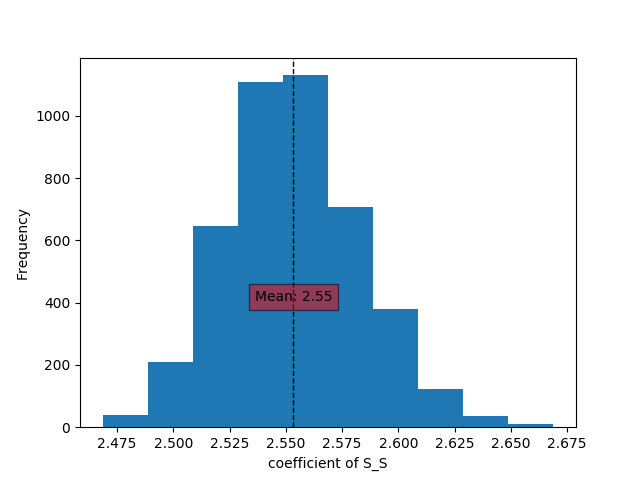
\includegraphics[width=6cm]{SS2.png}\par
				    		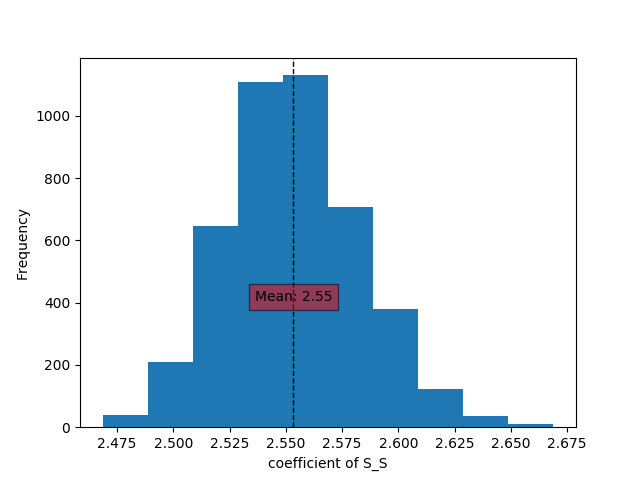
\includegraphics[width=6cm]{SS2.png}\par
				    		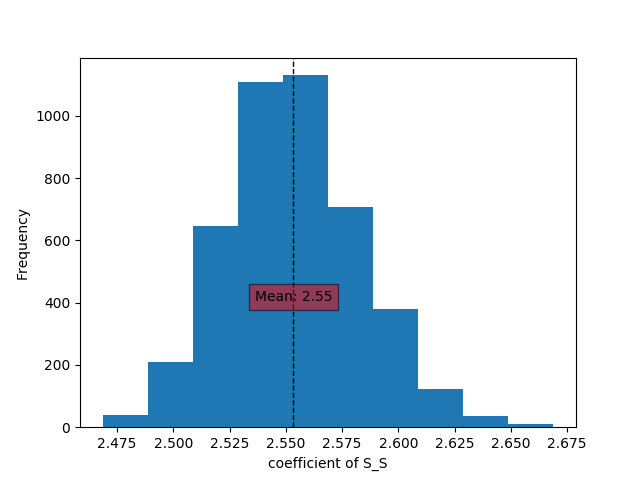
\includegraphics[width=6cm]{SS2.png}\par
				    	\end{multicols}   	 					\caption{Secondary-Secondary Carbon bond coefficient of sub-dataset}	  		  
				    	\label{plot:histstart}	 
				    	\begin{multicols}{3}
				    		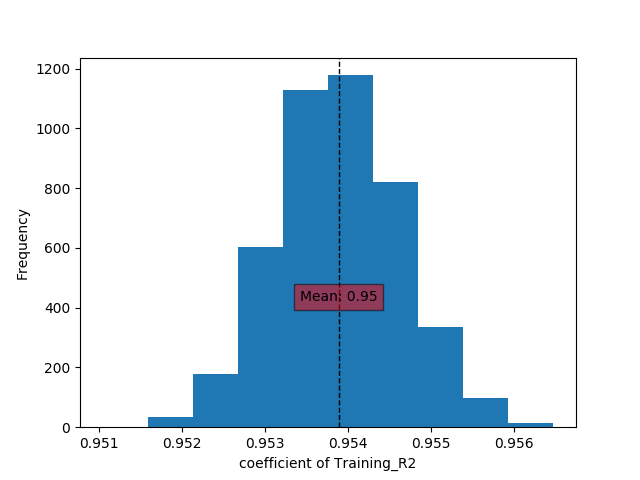
\includegraphics[width=6cm]{TrainingR20.png}\par 
				    		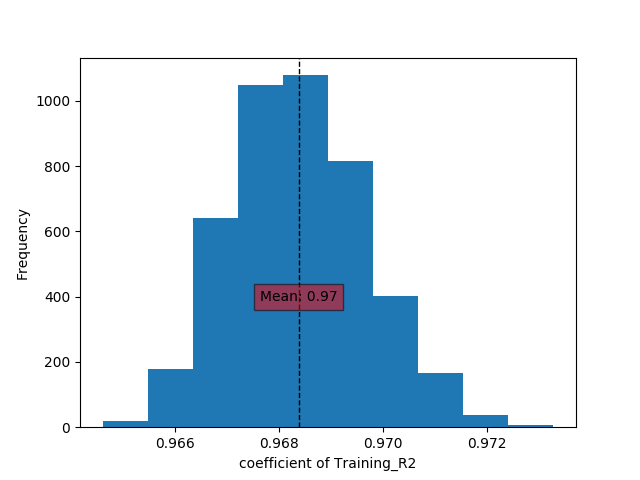
\includegraphics[width=6cm]{TrainingR21.png}\par 
				    		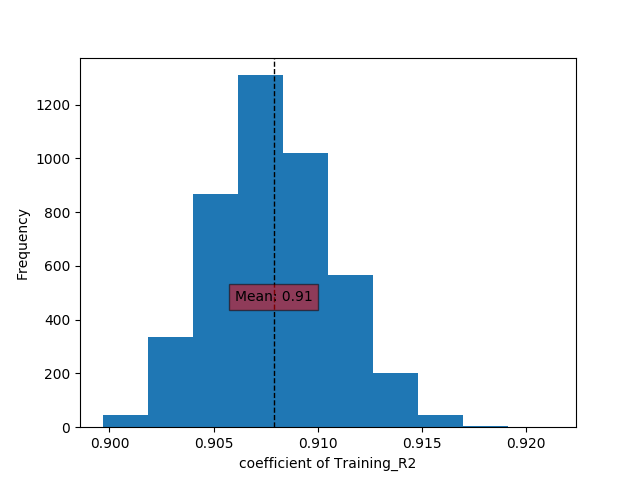
\includegraphics[width=6cm]{TrainingR22.png}\par 
				    	\end{multicols}		
				    	\caption{Training accuracy  of sub-dataset}	   		  
				    	\begin{multicols}{3}
				    		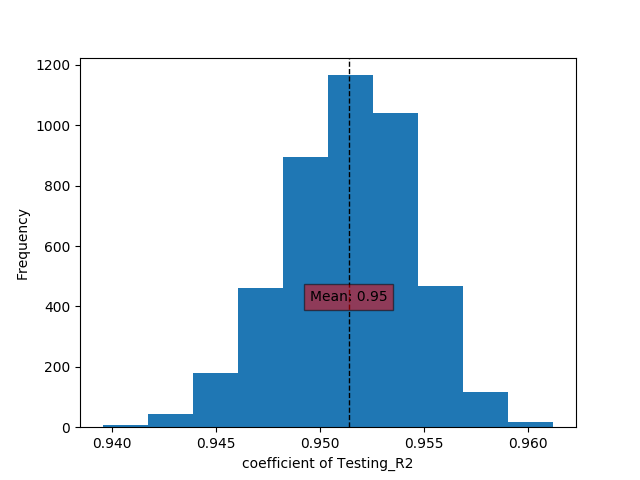
\includegraphics[width=6cm]{TestingR20.png}\par 
				    		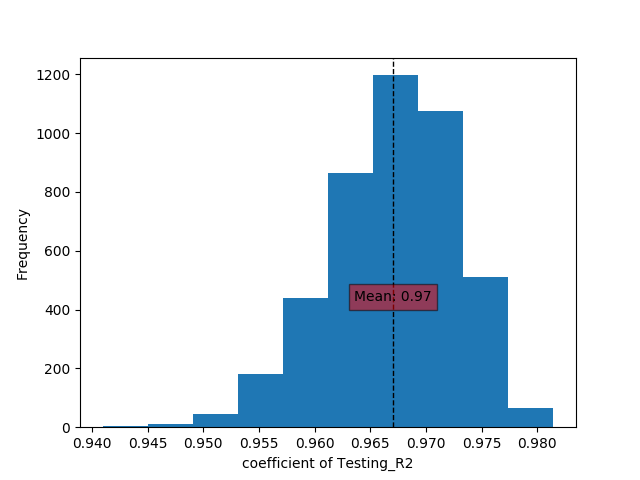
\includegraphics[width=6cm]{TestingR21.png}\par 
				    		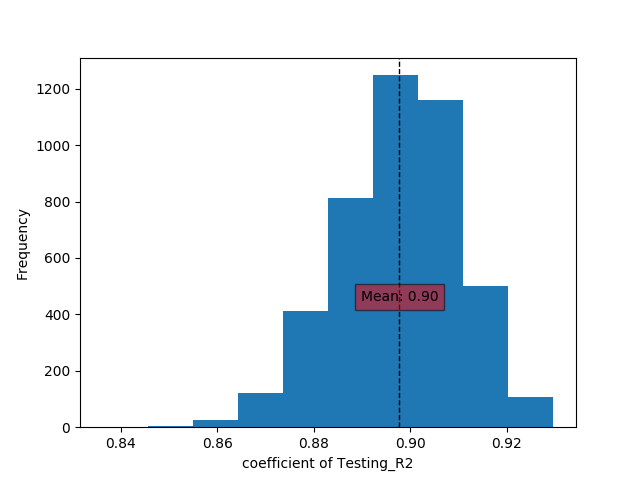
\includegraphics[width=6cm]{TestingR22.png}\par 
				    	\end{multicols}	
				    	\caption{Testing accuracy  of sub-dataset}	
				    	
				    \end{figure}
				    
				    
				    
				    \begin{figure}[H]
				    	\begin{multicols}{3}
				    		\centering
				    		Sub-dataset - 0 \par
				    		Sub-dataset - 1 \par
				    		Sub-dataset - 2 \par					
				    	\end{multicols}	  
				    	\begin{multicols}{3}				  	
				    		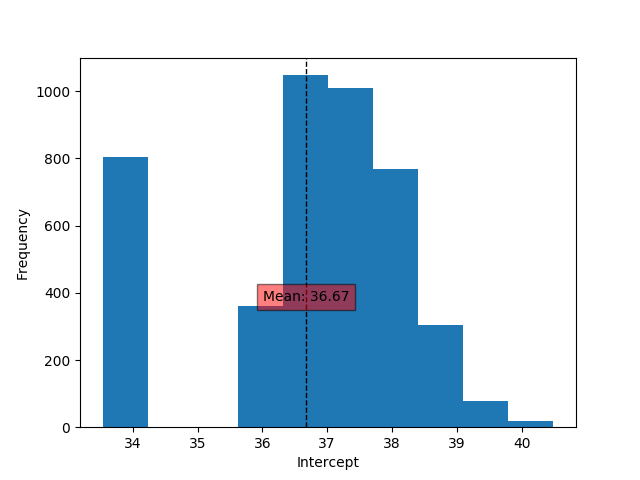
\includegraphics[width=6cm]{Constant0.png}\par 
				    		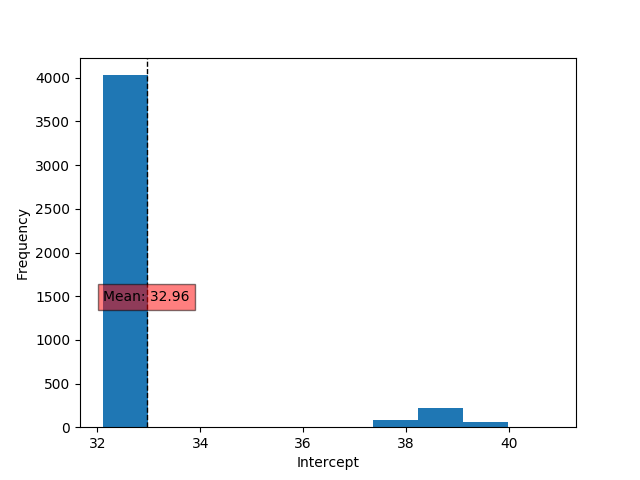
\includegraphics[width=6cm]{Constant1.png}\par 
				    		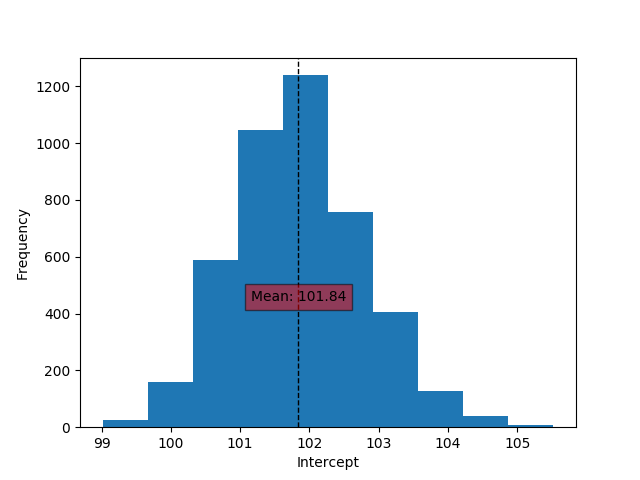
\includegraphics[width=6cm]{Constant2.png}\par 
				    	\end{multicols}
				    	\caption{Intercept of sub-dataset}									  	   				  	
				    	\begin{multicols}{3}
				    		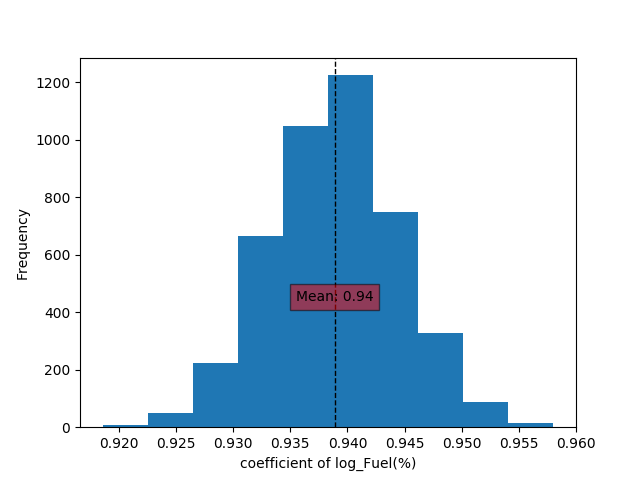
\includegraphics[width=6cm]{logFuel0.png}\par 
				    		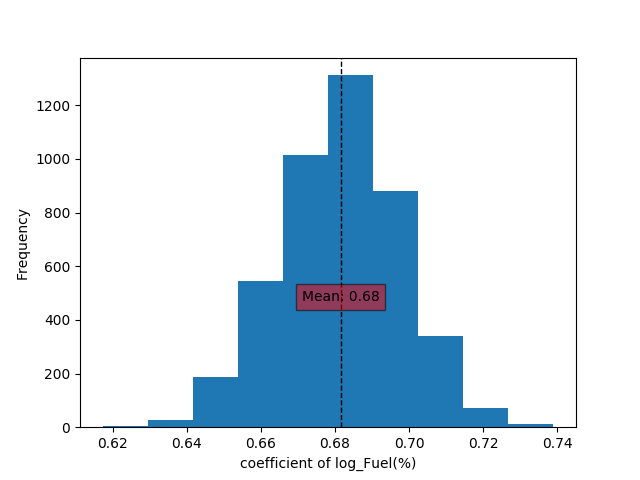
\includegraphics[width=6cm]{logFuel1.png}\par 
				    		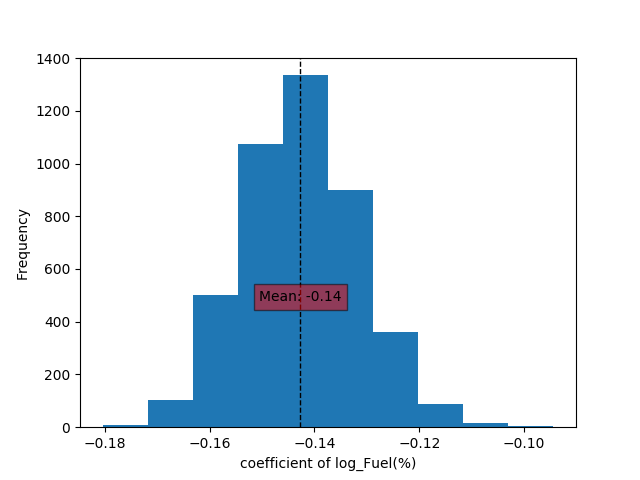
\includegraphics[width=6cm]{logFuel2.png}\par 
				    	\end{multicols}
				    	\caption{Fuel mole fraction term coefficient of sub-dataset}				  	
				    	\begin{multicols}{3}
				    		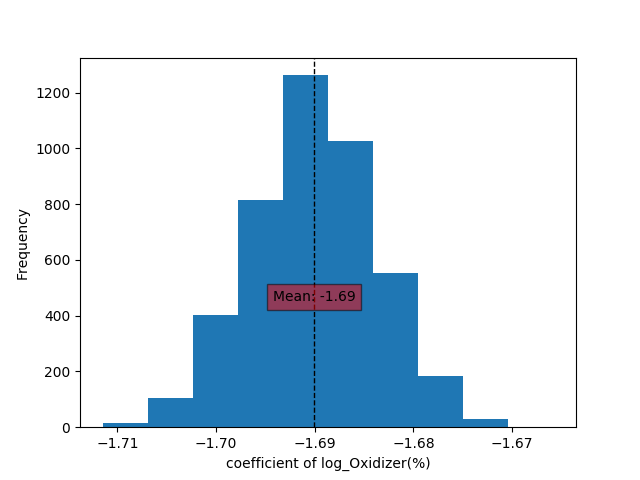
\includegraphics[width=6cm]{logOxidizer0.png}\par 
				    		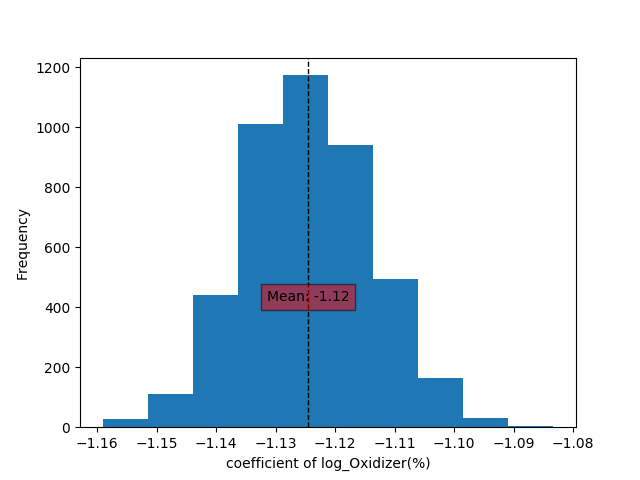
\includegraphics[width=6cm]{logOxidizer1.png}\par 
				    		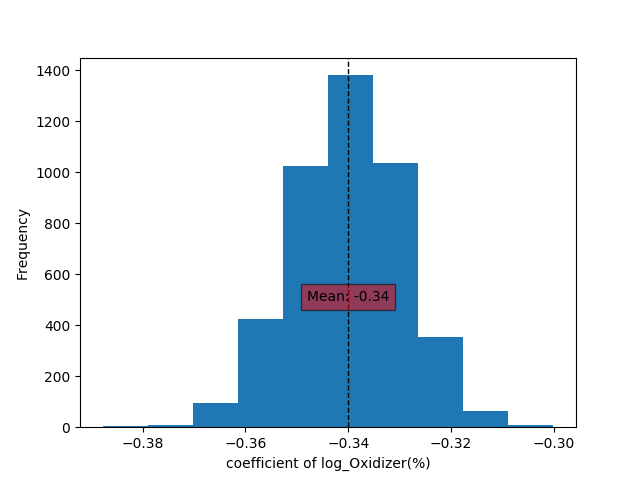
\includegraphics[width=6cm]{logOxidizer2.png}\par 
				    	\end{multicols}
				    	\caption{Oxygen  term coefficient of sub-dataset}
				    	\begin{multicols}{3}
				    		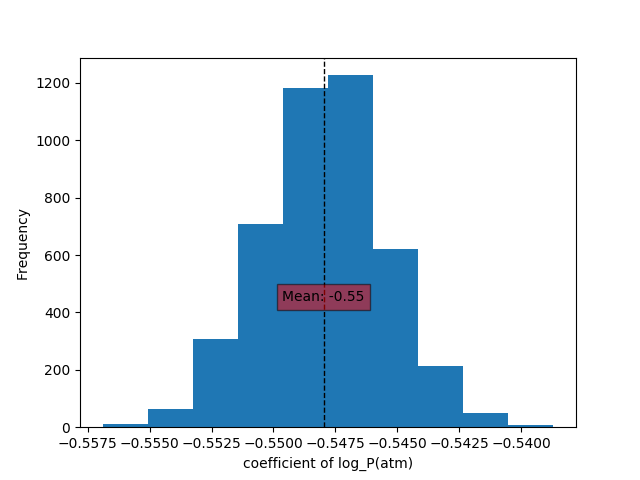
\includegraphics[width=6cm]{logP0.png}\par 
				    		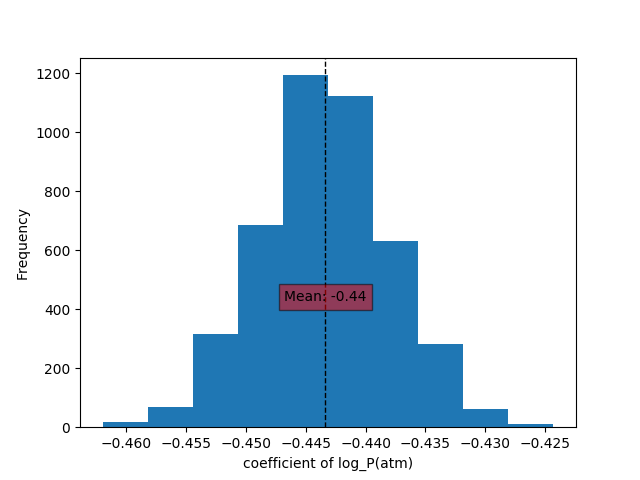
\includegraphics[width=6cm]{logP1.png}\par 
				    		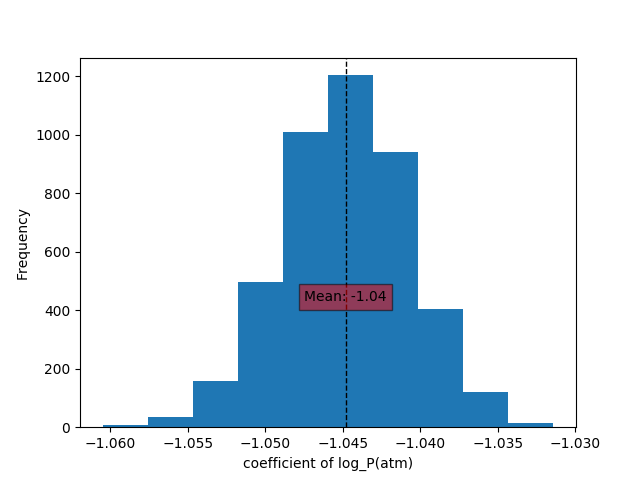
\includegraphics[width=6cm]{logP2.png}\par 
				    	\end{multicols}
				    	\caption{Pressure term coefficient of sub-dataset}			
				    \end{figure}
				    
				    
				    \begin{figure}	[H]
				    	\begin{multicols}{3}
				    		\centering
				    		Sub-dataset - 0 \par
				    		Sub-dataset - 1 \par
				    		Sub-dataset - 2 \par
				    	\end{multicols}	
				    	\begin{multicols}{3}
				    		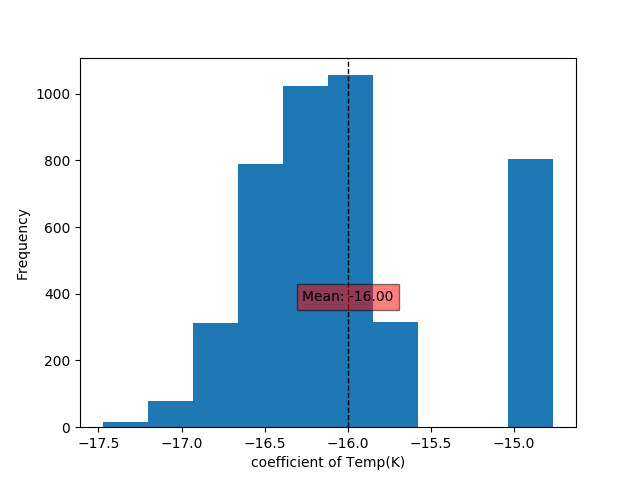
\includegraphics[width=6cm]{Temp0.png}\par 
				    		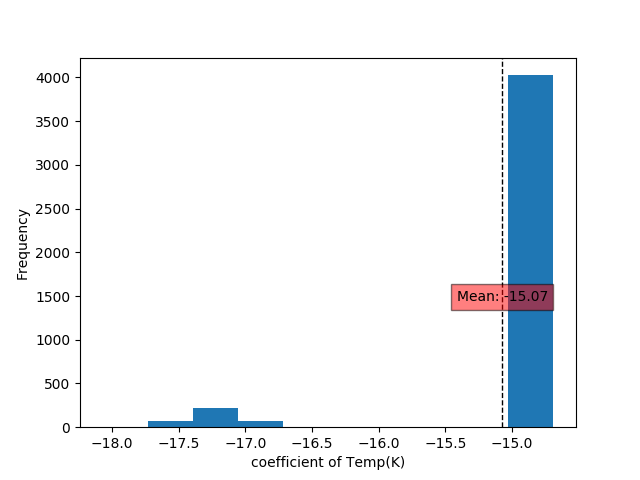
\includegraphics[width=6cm]{Temp1.png}\par 
				    		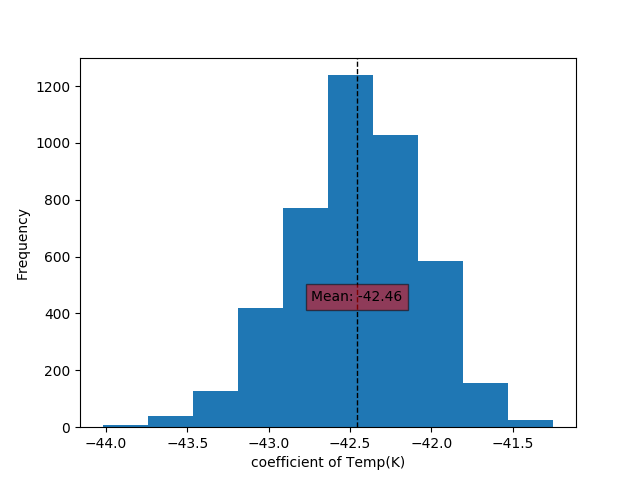
\includegraphics[width=6cm]{Temp2.png}\par 
				    	\end{multicols}
				    	\caption{Temperature term coefficient of sub-dataset}	  		  
				    	\begin{multicols}{3}
				    		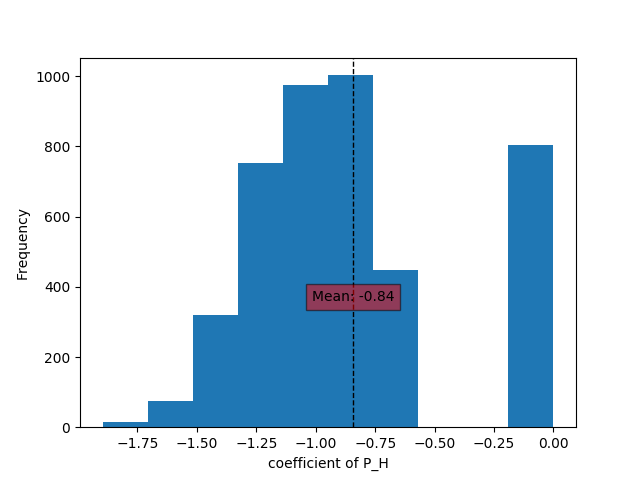
\includegraphics[width=6cm]{PH0.png}\par
				    		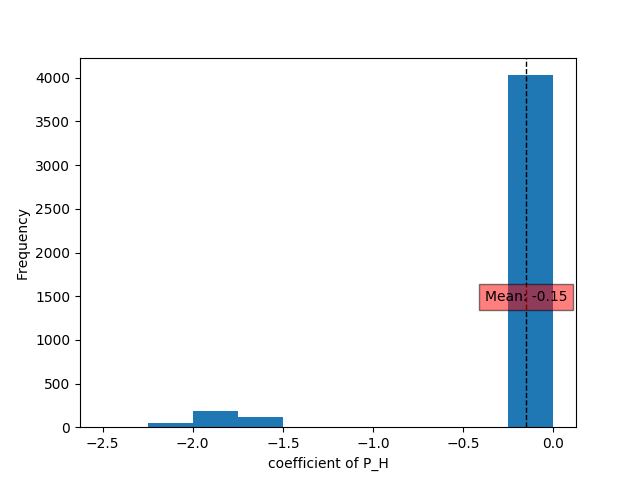
\includegraphics[width=6cm]{PH1.png}\par
				    		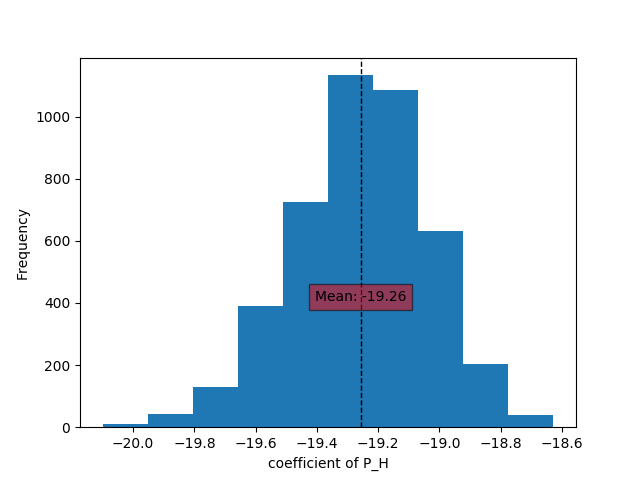
\includegraphics[width=6cm]{PH2.png}\par
				    	\end{multicols}
				    	\caption{Primary Carbon and Hydrogen bond coefficient of sub-dataset}	  		  
				    	\begin{multicols}{3}
				    		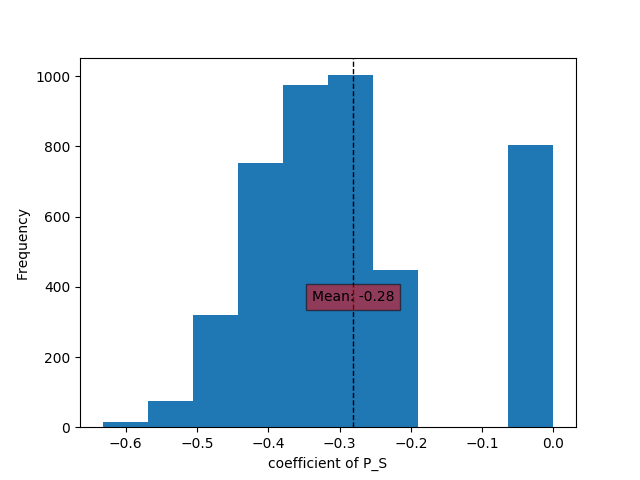
\includegraphics[width=6cm]{PS0.png}\par
				    		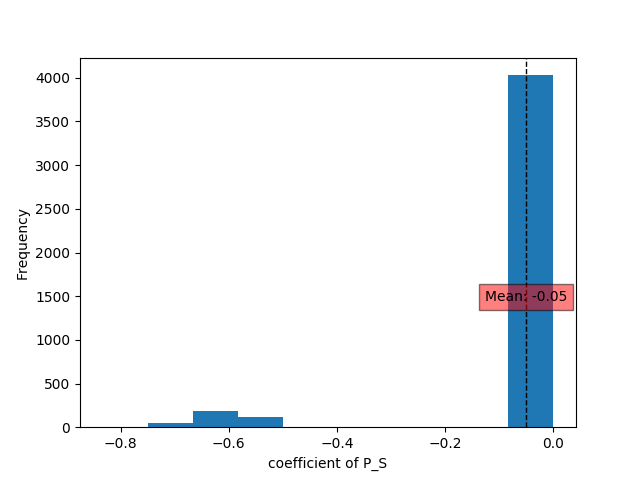
\includegraphics[width=6cm]{PS1.png}\par
				    		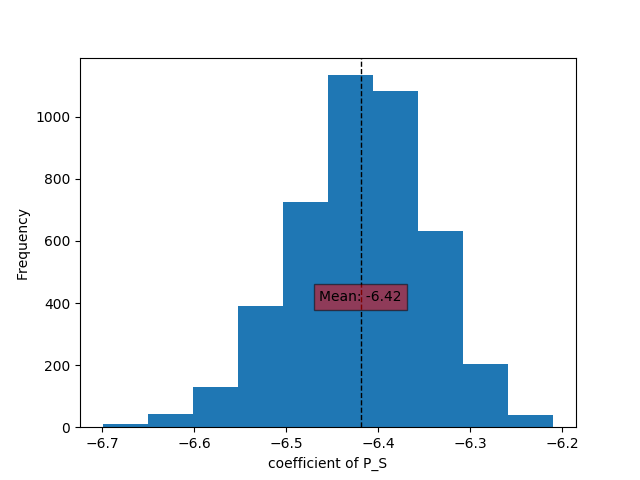
\includegraphics[width=6cm]{PS2.png}\par
				    	\end{multicols}				 					 \caption{Primary-Secondary Carbon bond coefficient of sub-dataset}	  		  
				    	\begin{multicols}{3}
				    		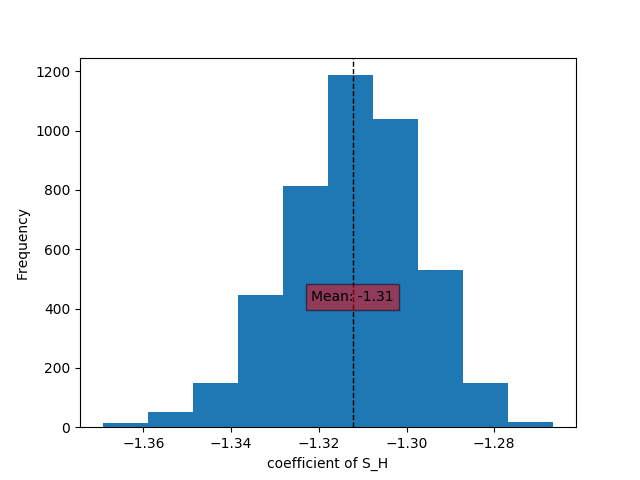
\includegraphics[width=6cm]{SH2.png}\par
				    		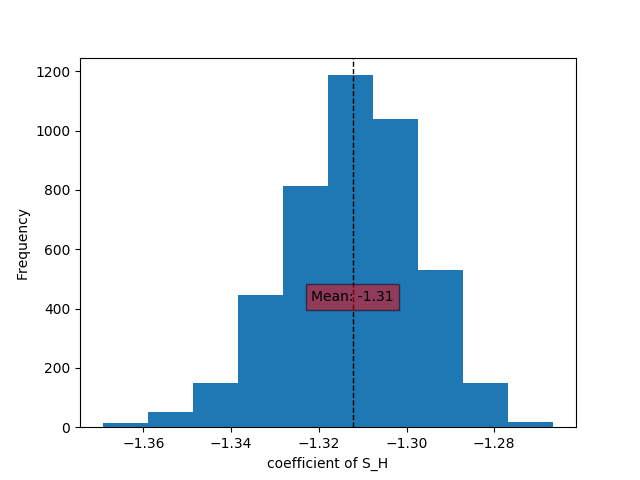
\includegraphics[width=6cm]{SH2.png}\par
				    		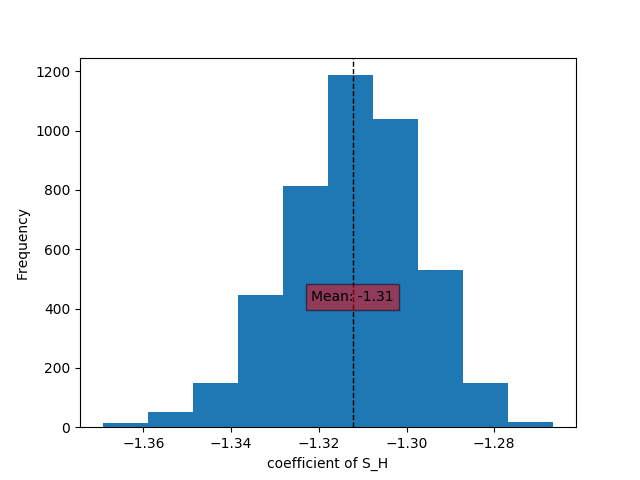
\includegraphics[width=6cm]{SH2.png}\par
				    	\end{multicols}
				    	\caption{Secondary Carbon and Hydrogen bond coefficient of sub-dataset}	  		  				 
				    	\label{plot:histend}	
				    \end{figure}
				    
				    Formulation of Ignition delay time is acquired using mean value of such distribution. After 4200 repetitive result mean value of coefficient converges to specific value as given in table-\ref{table:converge}. IDT correlation obtained from converged coefficient value- \ref{table:converge} is given as below. Associated value of centroids are mentioned in table-\ref{table:centroid} for 'all fuel' case:
				    
				   \begin{itemize}
						\item For centroid-0:							
						\begin{equation}\label{eq:c0}
					\tau = e^{36.68}\cdot 
					\bigg(\frac{T}{T_0}\bigg)^{-15.99}	\cdot
					\bigg(\frac{P}{P_0}\bigg)^{-0.55} \cdot
					X_{Fuel}^{0.94} \cdot
					X_{O_2}^{-1.69} \cdot
					e^{(C_PH)^{-0.84}} \cdot	
					e^{(C_PC_S)^{-0.28}} \cdot		
					e^{(C_SC_S)^{-0.13}} 					
						\end{equation}

						\item For centroid-1:							
						\begin{equation}\label{eq:c1}
						\tau = e^{32.96}\cdot 
						\bigg(\frac{T}{T_0}\bigg)^{-15.08}	\cdot
						\bigg(\frac{P}{P_0}\bigg)^{-0.44} \cdot
						X_{Fuel}^{0.68} \cdot
						X_{O_2}^{-1.12} \cdot
						e^{(C_PH)^{-0.16}} \cdot	
						e^{(C_PC_S)^{-0.05}} \cdot		
						e^{(C_SC_S)^{-0.29}} 					
						\end{equation}
						
						\item For centroid-2:							
						\begin{equation}\label{eq:c2}
						\tau = e^{101.85}\cdot 
						\bigg(\frac{T}{T_0}\bigg)^{-42.46}	\cdot
						\bigg(\frac{P}{P_0}\bigg)^{-1.04} \cdot
						X_{Fuel}^{-0.14} \cdot
						X_{O_2}^{-0.34} \cdot
						e^{(C_PH)^{-19.26}} \cdot	
						e^{(C_PC_S)^{-6.42}} \cdot		
						e^{(C_SC_S)^{-2.55}} \cdot
						e^{(C_SH)^{-1.31}}					
						\end{equation}
				   \end{itemize}
				   
				  		  \begin{table}[H]				  					   	\tiny 
				  		  	\begin{tabular}{|c|c|c|c|c|c|c|c|c|c|c|c|c|}
				  		  		\hline
				  		  		\textbf{} & \textbf{\begin{tabular}[c]{@{}c@{}}Number\\ of\\ Simulation\end{tabular}} & \textbf{Constant} & \textbf{P\_H} & \textbf{P\_S} & \textbf{S\_H} & \textbf{S\_S} & \textbf{Temp(K)} & \textbf{log\_Fuel(\%)} & \textbf{log\_Oxidizer(\%)} & \textbf{log\_P(atm)} & \textbf{Testing\_R2} & \textbf{Training\_R2} \\ \hline
				  		  		\multirow{10}{*}{\textbf{Cluster-0}} & 500 & 36.67 & -0.84 & -0.28 & 0 & 0.13 & -16 & 0.94 & -1.69 & -0.55 & 0.95 & 0.95 \\ \cline{2-13} 
				  		  		& 1000 & 36.72 & -0.86 & -0.29 & 0 & 0.13 & -16.02 & 0.94 & -1.69 & -0.55 & 0.95 & 0.95 \\ \cline{2-13} 
				  		  		& 1500 & 36.67 & -0.84 & -0.28 & 0 & 0.13 & -15.99 & 0.94 & -1.69 & -0.55 & 0.95 & 0.95 \\ \cline{2-13} 
				  		  		& 2000 & 36.66 & -0.84 & -0.28 & 0 & 0.13 & -15.99 & 0.94 & -1.69 & -0.55 & 0.95 & 0.95 \\ \cline{2-13} 
				  		  		& 2500 & 36.65 & -0.84 & -0.28 & 0 & 0.13 & -15.99 & 0.94 & -1.69 & -0.55 & 0.95 & 0.95 \\ \cline{2-13} 
				  		  		& 3000 & 36.65 & -0.84 & -0.28 & 0 & 0.13 & -15.99 & 0.94 & -1.69 & -0.55 & 0.95 & 0.95 \\ \cline{2-13} 
				  		  		& 3500 & 36.67 & -0.84 & -0.28 & 0 & 0.13 & -16 & 0.94 & -1.69 & -0.55 & 0.95 & 0.95 \\ \cline{2-13} 
				  		  		& 4000 & 36.68 & -0.85 & -0.28 & 0 & 0.13 & -15.99 & 0.94 & -1.69 & -0.55 & 0.95 & 0.95 \\ \cline{2-13} 
				  		  		& 4200 & 36.68 & -0.84 & -0.28 & 0 & 0.13 & -15.99 & 0.94 & -1.69 & -0.55 & 0.95 & 0.95 \\ \cline{2-13} 
				  		  		& 4395 & 36.68 & -0.84 & -0.28 & 0 & 0.13 & -15.99 & 0.94 & -1.69 & -0.55 & 0.95 & 0.95 \\ \hline
				  		  		\multirow{10}{*}{\textbf{Cluster-1}} & 500 & 33.16 & -0.21 & -0.07 & 0 & 0.28 & -15.15 & 0.68 & -1.12 & -0.44 & 0.97 & 0.97 \\ \cline{2-13} 
				  		  		& 1000 & 33.04 & -0.18 & -0.05 & 0 & 0.29 & -15.1 & 0.68 & -1.12 & -0.44 & 0.97 & 0.97 \\ \cline{2-13} 
				  		  		& 1500 & 33.01 & -0.17 & -0.06 & 0 & 0.29 & -15.09 & 0.68 & -1.12 & -0.44 & 0.97 & 0.97 \\ \cline{2-13} 
				  		  		& 2000 & 32.99 & -0.16 & -0.05 & 0 & 0.29 & -15.08 & 0.68 & -1.12 & -0.44 & 0.97 & 0.97 \\ \cline{2-13} 
				  		  		& 2500 & 32.98 & -0.16 & -0.05 & 0 & 0.29 & -15.08 & 0.68 & -1.12 & -0.44 & 0.97 & 0.97 \\ \cline{2-13} 
				  		  		& 3000 & 32.97 & -0.16 & -0.05 & 0 & 0.29 & -15.08 & 0.68 & -1.12 & -0.44 & 0.97 & 0.97 \\ \cline{2-13} 
				  		  		& 3500 & 32.97 & -0.16 & -0.05 & 0 & 0.29 & -15.08 & 0.68 & -1.12 & -0.44 & 0.97 & 0.97 \\ \cline{2-13} 
				  		  		& 4000 & 32.96 & -0.16 & -0.05 & 0 & 0.29 & -15.08 & 0.68 & -1.12 & -0.44 & 0.97 & 0.97 \\ \cline{2-13} 
				  		  		& 4200 & 32.96 & -0.16 & -0.05 & 0 & 0.29 & -15.08 & 0.68 & -1.12 & -0.44 & 0.97 & 0.97 \\ \cline{2-13} 
				  		  		& 4395 & 32.96 & -0.16 & -0.05 & 0 & 0.29 & -15.08 & 0.68 & -1.12 & -0.44 & 0.97 & 0.97 \\ \hline
				  		  		\multirow{10}{*}{\textbf{Cluster-2}} & 500 & 101.83 & -19.26 & -6.42 & -1.31 & 2.55 & -42.46 & -0.14 & -0.34 & -1.04 & 0.9 & 0.91 \\ \cline{2-13} 
				  		  		& 1000 & 101.85 & -19.26 & -6.42 & -1.31 & 2.55 & -42.46 & -0.14 & -0.34 & -1.04 & 0.9 & 0.91 \\ \cline{2-13} 
				  		  		& 1500 & 101.86 & -19.26 & -6.42 & -1.31 & 2.55 & -42.46 & -0.14 & -0.34 & -1.04 & 0.9 & 0.91 \\ \cline{2-13} 
				  		  		& 2000 & 101.84 & -19.26 & -6.42 & -1.31 & 2.55 & -42.46 & -0.14 & -0.34 & -1.04 & 0.9 & 0.91 \\ \cline{2-13} 
				  		  		& 2500 & 101.84 & -19.26 & -6.42 & -1.31 & 2.55 & -42.46 & -0.14 & -0.34 & -1.04 & 0.9 & 0.91 \\ \cline{2-13} 
				  		  		& 3000 & 101.86 & -19.26 & -6.42 & -1.31 & 2.55 & -42.46 & -0.14 & -0.34 & -1.04 & 0.9 & 0.91 \\ \cline{2-13} 
				  		  		& 3500 & 101.85 & -19.26 & -6.42 & -1.31 & 2.55 & -42.46 & -0.14 & -0.34 & -1.04 & 0.9 & 0.91 \\ \cline{2-13} 
				  		  		& 4000 & 101.84 & -19.26 & -6.42 & -1.31 & 2.55 & -42.46 & -0.14 & -0.34 & -1.04 & 0.9 & 0.91 \\ \cline{2-13} 
				  		  		& 4200 & 101.84 & -19.26 & -6.42 & -1.31 & 2.55 & -42.46 & -0.14 & -0.34 & -1.04 & 0.9 & 0.91 \\ \cline{2-13} 
				  		  		& 4395 & 101.85 & -19.26 & -6.42 & -1.31 & 2.55 & -42.46 & -0.14 & -0.34 & -1.04 & 0.9 & 0.91 \\ \hline
				  		  	\end{tabular}
				  		  	\vspace{0.25cm}
				  		  	\caption{Coefficient values obtained after given number of simulations for different sub-dataset which shows convergence of coefficient values}
				  		  	\label{table:converge}
				  		  \end{table}				  		  
				  		  For verification of correlation and frame work, smaller set dataset of heptane and hexadecane from, main dataset used to verify the result. All fuel data points used for training the model heptane and hexadecane are also part of it. After completer procedure mentioned as in \ref{fig:flowchart}, observed result shows excellent match with predicted value. For cluster-0,1 relative error is bounded between 0.8\%-3\% and 0.4\%-5\% respectively \ref{fig:all_fuel}. For cluster-2  error varied from 0.09\% to 16\% which is high as obtained coefficient of determination is also low.				  		  
				  		  
			  		    \begin{figure}[H]
			  		    	\centering
			  		    	\subfigure[IDT prediction of hexane and hexadecane fuel by Framework  using all fuel data   ]{\label{fig:WCSSE_dode}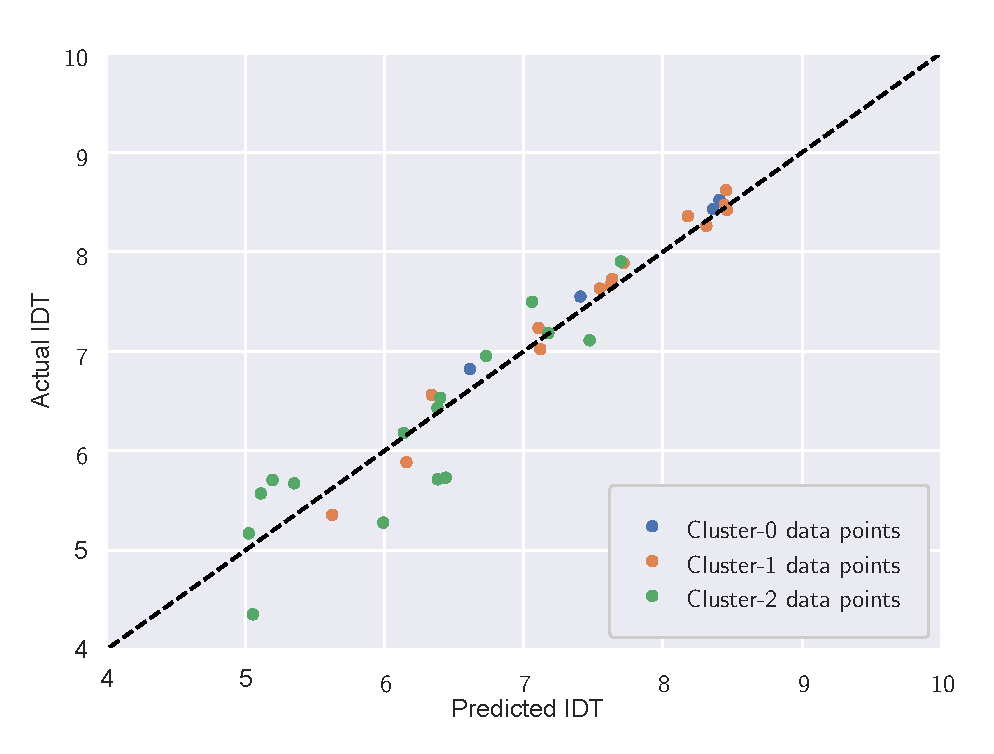
\includegraphics[scale=0.4]{igntionDelayFramework.eps}}
			  		    	\hspace{0.5cm}
			  		    	\subfigure[IDT prediction of hexane and hexadecane fuel using correlation using all fuel data ]{\label{fig:diff_cluster_dode}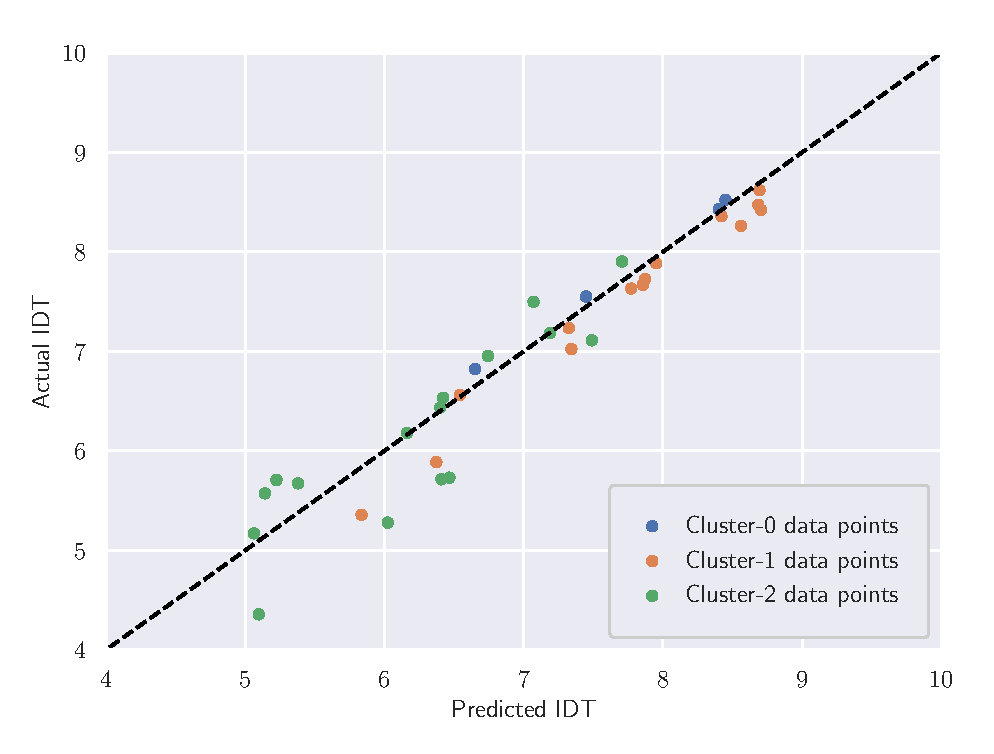
\includegraphics[scale=0.4]{igntionDelayCorrelation.eps}}
			  		    	\caption{Prediction of IDT of hexane and hexadecane using correlation and Framework}
			  		    	\label{fig:all_fuel}
			  		    \end{figure}
			  		    
			  		  	  Result of IDT from correlation shows slightly more deviation. But it follows the same trend as of framework result. Good prediction of hexane and hexadecane is expected as correlation already contains those fuel detail. The goal is present  study is to  predict IDT for new unknown fuel.
				  		  	  
				  		  To check prediction of unknown straight chain alkane fuel, Hexadecane and Hexane is used as unknown fuel which would not be part of training and testing set. Model is trained using remaining all fuel. To attain main objective and check behaviour of framework as well as correlational result are mentioned in figure-\ref{fig:unknown}. 
				  		  
				  		  \begin{figure}[H]
				  		  	\centering
				  		  	\subfigure[IDT prediction of hexane and hexadecane fuel by Framework  using fuel other than hexane and hexadecane]{\label{fig:WCSSE_dode}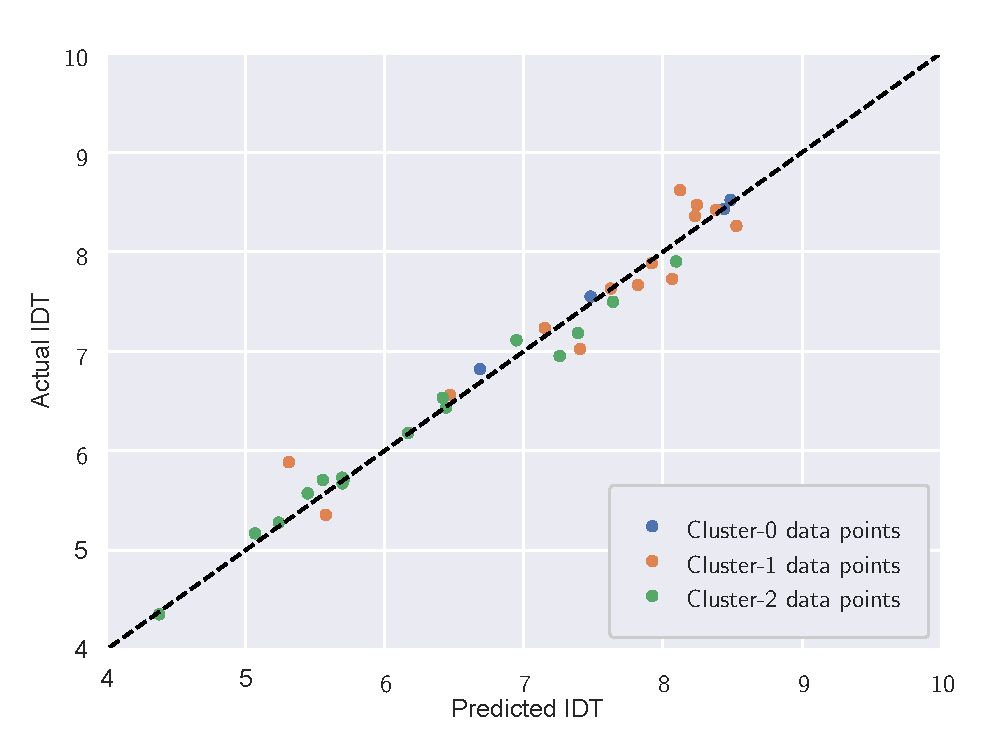
\includegraphics[scale=0.4]{igntiondelayframeworkNHH.eps}}
				  		  	\hspace{0.5cm}
				  		  	\subfigure[IDT prediction of hexane and hexadecane fuel using correlation using fuel other than hexane and hexadecane. ]{\label{fig:diff_cluster_dode}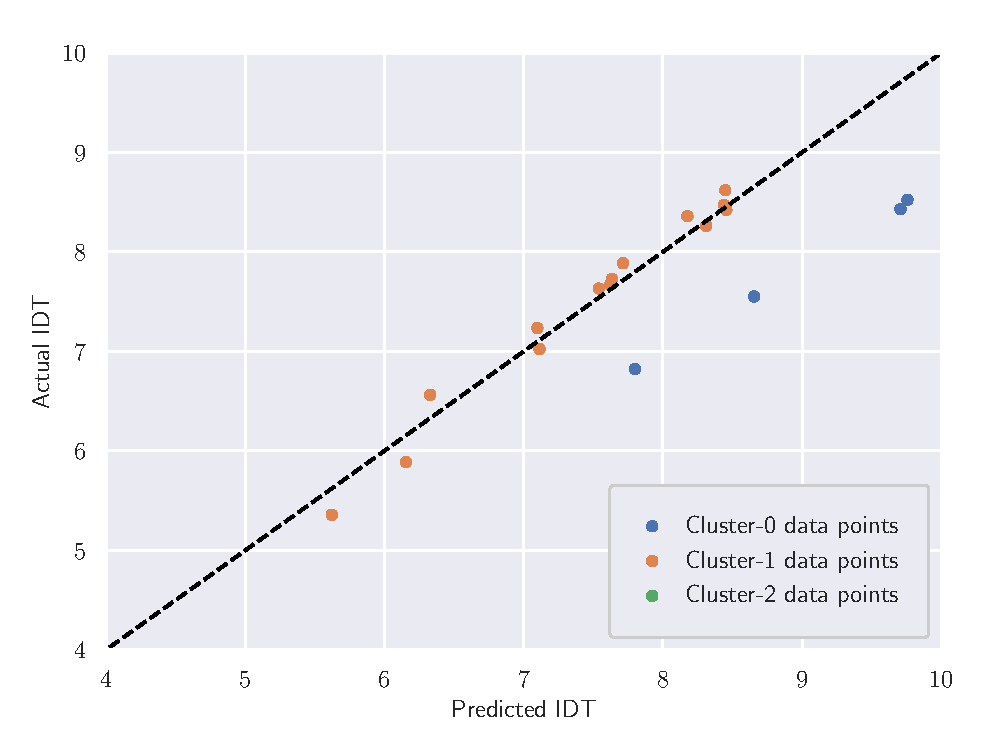
\includegraphics[scale=0.4]{igntiondelaycorrelationNHH.eps}}
				  		  	\caption{Prediction of IDT of hexane and hexadecane using correlation and Framework}
				  		  	\label{fig:unknown}
				  		  \end{figure}
				  		  
				  		  Result of figure-\ref{fig:unknown} shows that prediction using framework again gives excellent fit but result obtained using correlation incurred considerable error in prediction. Error in correlation result might be caused due to the  movement of centroids which shows that Accuracy of correlational depends also on centroid value. 				  					  		  
				  		   
				  		   \begin{figure}[H]
				  		   	\centering
				  		   	\subfigure[IDT prediction of all fuel other than propane, heptane and dodeacne by Framework  using propane, heptane and dodeacne as learning set]{\label{fig:WCSSE_dode}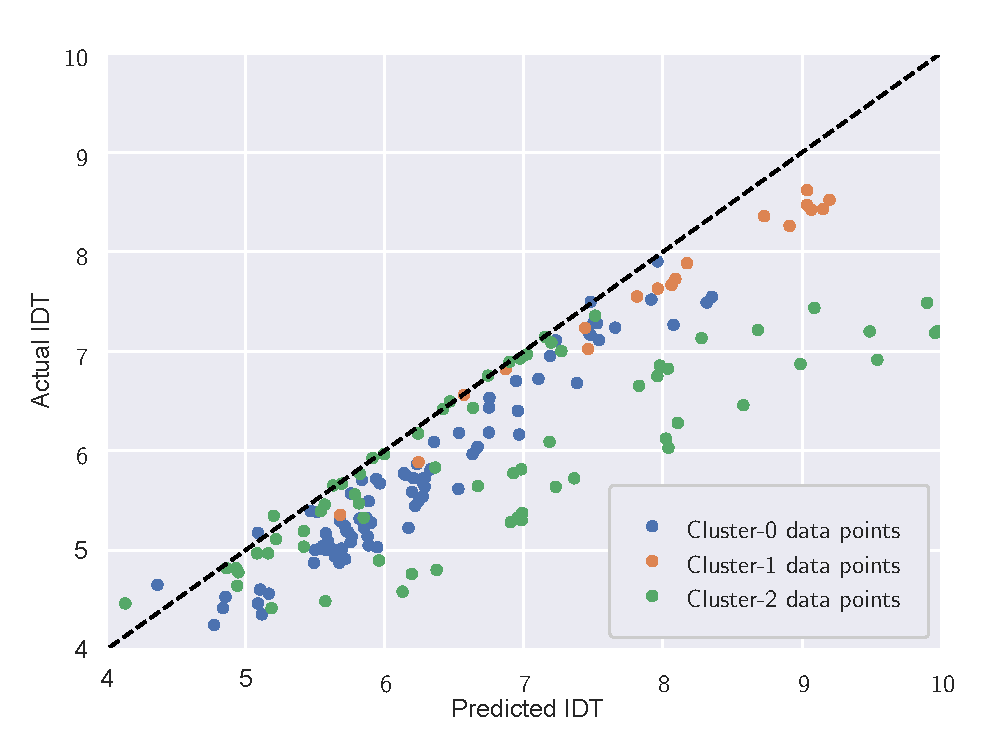
\includegraphics[scale=0.40]{3fuelFramework.eps}}
				  		   	\hspace{0.5cm}
				  		   	\subfigure[IDT prediction of all fuel other than propane, heptane and dodeacne using correlation using propane, heptane and dodeacne as learning set. ]{\label{fig:diff_cluster_dode}\includegraphics[scale=0.40]{3FuelCorrelation.eps}}
				  		   	\caption{Prediction of IDT of hexane and hexadecane using correlation and Framework}
				  		   	\label{fig:3fuel}
				  		   \end{figure}

				  		  
				  		    To verify extreme case, propane, heptane and dodecane were used to train the model as it almost covers wide range of condition and different length of alkanes. Rest of all fuel were used as unknown fuel to test the prediction. Observed result was quite unexpected, which is shown in fig-\ref{fig:3fuel}. Obtained result from framework is quite scattered specifically for cluster-2. Whereas result obtained using correlation \ref{eq:c0},\ref{eq:c1},\ref{eq:c2} shows excellent agreement of predicted result with experimental result. Centroids were obtained from propane, heptane and dodecane. Such pair of centroid and correlation is important for prediction IDT of new fuel. 
				  
%				    \begin{figure}[H]	
%				    	\begin{multicols}{3}
%				    		\centering
%				    		Sub-dataset - 0 \par
%				    		Sub-dataset - 1 \par
%				    		Sub-dataset - 2 \par
%				    	\end{multicols}	
%				    	\begin{multicols}{3}
%				    		\includegraphics[width=6cm]{SS2.png}\par
%				    		\includegraphics[width=6cm]{SS2.png}\par
%				    		\includegraphics[width=6cm]{SS2.png}\par
%				    	\end{multicols}   					    	\label{plot:histend}	  					\caption{Secondary-Secondary Carbon bond coefficient of sub-dataset}	  		  
%				    	\begin{multicols}{3}
%				    		\includegraphics[width=6cm]{TrainingR20.png}\par 
%				    		\includegraphics[width=6cm]{TrainingR21.png}\par 
%				    		\includegraphics[width=6cm]{TrainingR22.png}\par 
%				    	\end{multicols}		
%				    	\caption{Training accuracy  of sub-dataset}	   		  
%				    	\begin{multicols}{3}
%				    		\includegraphics[width=6cm]{TestingR20.png}\par 
%				    		\includegraphics[width=6cm]{TestingR21.png}\par 
%				    		\includegraphics[width=6cm]{TestingR22.png}\par 
%				    	\end{multicols}	
%				    	\caption{Testing accuracy  of sub-dataset}	
%
%				    \end{figure}
%				    
%				    
%				  		  
%				  \begin{figure}[H]
%				  	  \begin{multicols}{3}
%				  	  \centering
%				  	  	Sub-dataset - 0 \par
%				  	  	Sub-dataset - 1 \par
%						Sub-dataset - 2 \par					
%				  	  \end{multicols}	  
%				  \begin{multicols}{3}				  	
%				  	\includegraphics[width=6cm]{Constant0.png}\par 
%				  	\includegraphics[width=6cm]{Constant1.png}\par 
%				  	\includegraphics[width=6cm]{Constant2.png}\par 
%				  \end{multicols}
%					\caption{Intercept of sub-dataset}									  	 \label{plot:histstart}	  				  	
%				\begin{multicols}{3}
%					\includegraphics[width=6cm]{logFuel0.png}\par 
%					\includegraphics[width=6cm]{logFuel1.png}\par 
%					\includegraphics[width=6cm]{logFuel2.png}\par 
%				\end{multicols}
%				\caption{Fuel mole fraction term coefficient of sub-dataset}				  	
%				\begin{multicols}{3}
%					\includegraphics[width=6cm]{logOxidizer0.png}\par 
%					\includegraphics[width=6cm]{logOxidizer1.png}\par 
%					\includegraphics[width=6cm]{logOxidizer2.png}\par 
%				\end{multicols}
%				\caption{Oxygen  term coefficient of sub-dataset}
%				\begin{multicols}{3}
%					\includegraphics[width=6cm]{logP0.png}\par 
%					\includegraphics[width=6cm]{logP1.png}\par 
%					\includegraphics[width=6cm]{logP2.png}\par 
%				\end{multicols}
%				\caption{Pressure term coefficient of sub-dataset}			
%				\end{figure}
%				
%
%				 \begin{figure}	[H]
%				 	 \begin{multicols}{3}
%				 	 	\centering
%				 	 	Sub-dataset - 0 \par
%				 	 	Sub-dataset - 1 \par
%				 	 	Sub-dataset - 2 \par
%				 	 \end{multicols}	
%				 	 	\begin{multicols}{3}
%				 	 		\includegraphics[width=6cm]{Temp0.png}\par 
%				 	 		\includegraphics[width=6cm]{Temp1.png}\par 
%				 	 		\includegraphics[width=6cm]{Temp2.png}\par 
%				 	 	\end{multicols}
%				 	 	\caption{Temperature term coefficient of sub-dataset}	  		  
%				 	\begin{multicols}{3}
%				 		\includegraphics[width=6cm]{PH0.png}\par
%				 		\includegraphics[width=6cm]{PH1.png}\par
%				 		\includegraphics[width=6cm]{PH2.png}\par
%				 	\end{multicols}
%				 \caption{Primary Carbon and Hydrogen bond coefficient of sub-dataset}	  		  
%				 	\begin{multicols}{3}
%				 		\includegraphics[width=6cm]{PS0.png}\par
%				 		\includegraphics[width=6cm]{PS1.png}\par
%				 		\includegraphics[width=6cm]{PS2.png}\par
%				 	\end{multicols}				 					 \caption{Primary-Secondary Carbon bond coefficient of sub-dataset}	  		  
%				 	\begin{multicols}{3}
%				 		\includegraphics[width=6cm]{SH2.png}\par
%				 		\includegraphics[width=6cm]{SH2.png}\par
%				 		\includegraphics[width=6cm]{SH2.png}\par
%				 	\end{multicols}
%				 \caption{Secondary Carbon and Hydrogen bond coefficient of sub-dataset}	  		  				 
%				 			 	
%				 \end{figure}
%				 
				
				
				  
				  
				 %%%%%%%%%%%%%%%%%%%%%%%%%%%%%%%%%%%%
				 %%%%%%%%%%   ALGORITHM     %%%%%%%%%
				 %%%%%%%%%%%%%%%%%%%%%%%%%%%%%%%%%%%%
				  % Define block styles
				  \tikzstyle{decision} = [diamond, draw, fill=blue!20, 
				  text width=4.5em, text badly centered, node distance=3cm, inner sep=0pt]
				  \tikzstyle{block} = [rectangle, draw, fill=blue!15, 
				  text width=7em, text centered, rounded corners, minimum height=5em]
				  \tikzstyle{line} = [draw, -latex']
				  \tikzstyle{cloud} = [draw, ellipse,fill=red!20, node distance=3cm,
				  minimum height=2em]
				  \begin{figure}[H]
				  \centering
				  \begin{tikzpicture}[node distance = 2.7cm, auto]
				  % Place nodes
				  \node [block] (init) {Data Collection and Procesing};
 				  \node [block, below of=init] (processed) {Processed Dataset };
 				  \node [block, right of=processed,node distance=4cm] (shiloutte) {Silhouette Criteria and Elbow method};
 				  \node [block, below of=shiloutte] (cluster) {Number of clusters = 3};
%				  \node [cloud, left of=init] (expert) {expert};
%				  \node [cloud, right of=init] (system) {system};
				  \node [block, below of=processed] (kmeans) {K-Means Algorithm};
				  \node [block, below of=kmeans] (subdata2) {Sub-dataset:2};
				  \node [block, left of=subdata2,node distance=4cm] (subdata1) {Sub-dataset:1};
				  \node [block, right of=subdata2,node distance=4cm] (subdata3) {Sub-dataset:3};
				  
				  %%%subdataset -1
  				  \node [block, below of=subdata1] (generation1) {Data point generation and sampling in Sub-dataset:1};
  				  \node [block, below of=generation1] (mr1) {Muliple Regression of Sub-dataset:1};
				  \node [block, below of=mr1] (hypo1) {Hypothesis Testing based on p-value};
				  \node [block, below of=hypo1] (IDT1) {Igntion Delay Correlation-1};
				  
				  %%%subdataset -2
				  \node [block, below of=subdata2] (generation2) {Data point generation and sampling in Sub-dataset:2};
				  \node [block, below of=generation2] (mr2) {Muliple Regression of Sub-dataset:2};
				  \node [block, below of=mr2] (hypo2) {Hypothesis Testing based on p-value};
				  \node [block, below of=hypo2] (IDT2) {Igntion Delay Correlation-2};
				  
				  %%%subdataset -3
				  \node [block, below of=subdata3] (generation3) {Data point generation and sampling in Sub-dataset:3};
				  \node [block, below of=generation3] (mr3) {Muliple Regression of Sub-dataset:3};
				  \node [block, below of=mr3] (hypo3) {Hypothesis Testing based on p-value};
				  \node [block, below of=hypo3] (IDT3) {Igntion Delay Correlation-3};
				  
%				  \node [block, left of=evaluate, node distance=3cm] (update) {update model};
%				  \node [decision, below of=evaluate] (decide) {is best candidate better?};
%				  \node [block, below of=decide, node distance=3cm] (stop) {stop};
				  % Draw edges
				  \path [line] (init) -- (processed);				  				  
				  \path [line] (processed) |- (shiloutte);
				  \path [line] (shiloutte) -- (cluster);
				  \path [line] (processed) -- (kmeans);
  				  \path [line] (cluster) -- (kmeans);
  				  \path [line] (kmeans) -- (subdata2);
  				  \path [line] (kmeans) -- (subdata1);
  				  \path [line] (kmeans) -- (subdata3);   				  				  %%%subdataset -1				  
  				  \path [line] (subdata1) -- (generation1);
  				  \path [line] (generation1) -- (mr1);  
  				  \path [line] (mr1)--(hypo1); 
  				  \path [line] (hypo1)--(mr1); 
  				  \path [line] (hypo1) -- (IDT1); 
  				  
  				  %%%subdataset -2			  
  				  \path [line] (subdata2) -- (generation2);
  				  \path [line] (generation2) -- (mr2);  
  				  \path [line] (mr2)--(hypo2); 
  				  \path [line] (hypo2)--(mr2); 
  				  \path [line] (hypo2) -- (IDT2);
  				  
  				  %%%subdataset -1				  
  				  \path [line] (subdata3) -- (generation3);
  				  \path [line] (generation3) -- (mr3);  
  				  \path [line] (mr3)--(hypo3); 
  				  \path [line] (hypo3)--(mr3); 
  				  \path [line] (hypo3) -- (IDT3);
				 \end{tikzpicture}
				 \vspace{0.5cm}
				 \caption{Flowchart of Ignition Delay Time Prediction Framework }
				 \label{fig:flowchart}
				  \end{figure}
				 
			
			
  

							
						
					
						 
					
					
				
				\newpage	
			References:
					%%
					%% Following citation commands can be used in the body text:
					%% Usage of \cite is as follows:
					
					%%   \cite{key}          ==>>  [#]
					%%   \cite[chap. 2]{key} ==>>  [#, chap. 2]
					%%   \citet{key}         ==>>  Author [#]
					
					%% References with bibTeX database:
					
					\bibliographystyle{ieeetr}
					\bibliography{biblio.bib}
					
					%% Authors are advised to submit their bibtex database files. They are
					%% requested to list a bibtex style file in the manuscript if they do
					%% not want to use model1-num-names.bst.
					
					%% References without bibTeX database:
					
					% \begin{thebibliography}{00}
					
					%% \bibitem must have the following form:
					%%   \bibitem{key}...
					%%
					
					% \bibitem{}
					
					% \end{thebibliography}
					
					
				\end{document}
				
				%%
				%% End of file `elsarticle-template-1-num.tex'.